%; whizzy paragraph
%; whizzy-paragraph "^\\\\dancersection"
% -initex iniptex -latex platex -format platex -bibtex jbibtex -fmt fmt
% $B0J>e(B whizzytex $B$r;HMQ$9$k>l9g$N@_Dj!#(B

%     Tokyo Debian Meeting resources
%     Kansai Debian Meeting resources
%     Copyright (C) 2008 Junichi Uekawa
%     Copyright (C) 2008 Nobuhiro Iwamatsu

%     This program is free software; you can redistribute it and/or modify
%     it under the terms of the GNU General Public License as published by
%     the Free Software Foundation; either version 2 of the License, or
%     (at your option) any later version.

%     This program is distributed in the hope that it will be useful,
%     but WITHOUT ANY WARRANTY; without even the implied warranty of
%     MERCHANTABILITY or FITNESS FOR A PARTICULAR PURPOSE.  See the
%     GNU General Public License for more details.

%     You should have received a copy of the GNU General Public License
%     along with this program; if not, write to the Free Software
%     Foundation, Inc., 51 Franklin St, Fifth Floor, Boston, MA  02110-1301 USA

%   Pdf$B:n@.<j=g(B
% dvipdfmx debianmeetingresume2011-fuyu.dvi
%  preview (shell-command (concat "evince " (replace-regexp-in-string "tex$" "pdf"(buffer-file-name)) "&"))
% $B2hA|%U%!%$%k$r=hM}$9$k$?$a$K$O(Bebb$B$rMxMQ$7$F(Bboundingbox$B$r:n@.!#(B
%(shell-command "cd image2012-fuyu; ebb *.png")


% progress memo:
% 2015/6-2015/11$B$,%^!<%8BP>](B
% $B%$%Y%s%HEy$G$J$$>l9g$OM}M3$r=q$/$3$H!#(B
% $BI,MW$JJQ99E@$O(B FIXME $B$G5-O?$7$F$$$^$9!#(B

%%$B$3$3$+$i%X%C%@3+;O!#(B

\documentclass[mingoth,a4paper]{jsarticle}
\usepackage{monthlyreport}
\usepackage[dvips]{xy} % for advi workaround. Bug #452044
\usepackage{iwamatsu}
\usepackage{ulem}

% $B%Z!<%8D4@0$N$?$aItJ,E*$K(B2$BCJAH$K(B
\usepackage{multicol}

\begin{document}

\begin{titlepage}
\thispagestyle{empty}

\hspace*{-2.5cm}
\includegraphics{image2012-natsu/gudeb.eps}\\
\\
\\
\rotatebox{10}{\fontsize{32}{32} {\gt $BEl5~%(%j%"(B/$B4X@>#D#e#b#i#a#nJY6/2q(B}}

%\vspace*{-1.5cm}
\hspace*{11cm}
\includegraphics[height=6cm]{image200502/openlogo-nd.eps}\\
\vspace*{0.1cm}
\hfill $B$"$s$I$-$e$a$s$F$C$I(B $B$G$S$"$s(B 2015$BG/E_9f(B 2015$BG/(B12$B7n(B31$BF|(B $B=iHGH/9T(B
\end{titlepage}

\newpage
\thispagestyle{empty}\mbox{}
\newpage

% section $B$NBe$o$j$N4D6-(B -- $B2~D{$9$k!#(B
\renewcommand{\dancersection}[2]{%
\newpage
$B$"$s$I$-$e$a$s$F$C$I(B $B$G$S$"$s(B 2015$BG/E_9f(B
%
% top line
\vspace{0.1mm}\\
{\color{dancerlightblue}\rule{\hsize}{2mm}}

%
% middle text
%
\begin{minipage}[t]{0.6\hsize}
\color{dancerdarkblue}
\vspace{1cm}
\section{#1}
\hfill{}#2\\
\end{minipage}
\begin{minipage}[t]{0.4\hsize}
\vspace{-2cm}
\hfill{}
\includegraphics[height=8cm]{image200502/openlogo-nd.eps}\\
\vspace{-5cm}
\end{minipage}
%
%
{\color{dancerdarkblue}\rule{0.74\hsize}{2mm}}
%
\vspace{2cm}
}

\setcounter{page}{1}
\begin{minipage}[]{0.2\hsize}
 \definecolor{titleback}{gray}{0.9}
 \colorbox{dancerlightblue}{\rotatebox{90}{\fontsize{80}{80}
{\gt \color{dancerdarkblue}$B%G%S%"%sJY6/2q(B} }}
\end{minipage}
\begin{minipage}[]{0.8\hsize}
\hrule
\vspace{1mm}
\hrule
\setcounter{tocdepth}{1}
{\small
 \tableofcontents}
\vspace{1mm}
\hrule
\vspace{3cm}

\end{minipage}

% FIXME: $BK\J8$rDI2C$9$k$3$H!#(B
%-------------------------------------------------------------------------------
\dancersection{Introduction}{DebianJP}
%-------------------------------------------------------------------------------

\subsection{$BEl5~%(%j%"(BDebian$BJY6/2q(B}

 Debian$BJY6/2q$X$h$&$3$=!#$3$l$+$i(BDebian$B$N@$3&$K$"$7$rF'$_F~$l$k$H(B
 $B$$$&J}$b!"$9$G$K$I$C$W$j$H$D$+$C$F$$$k$H$$$&J}$b!"7n$K0l2s(BDebian$B$K$D$$(B
 $B$F8l$j$^$;$s$+!)(B

 Debian$BJY6/2q$NL\E*$O2<5-$G$9!#(B

\begin{itemize}
 \item \underline{Debian Developer} ($B3+H/<T(B)$B$N0i@.!#(B
 \item $BF|K\8l$G$N(B ``\underline{$B3+H/$K4X$9$k>pJs(B}'' $B$r@0M}$7$F$^$H$a!"%"%C%W%G!<%H$9$k!#(B
 \item \underline{$B>l(B}$B$NDs6!!#(B
 \begin{itemize}
  \item $BIaCJ$P$i$P$i$J>l=j$K$$$k?M!9$,(B face-to-face $B$G=P2q$($k>l$rDs6!(B
    $B$9$k!#(B
  \item Debian $B$N$?$a$K$J$k$3$H$r8l$k>l$rDs6!$9$k!#(B
  \item Debian$B$K$D$$$F8l$k>l$rDs6!$9$k!#(B
 \end{itemize}
\end{itemize}

 Debian$B$NJY6/2q$H$$$&$3$H$G5f6KE*$K$O;22C<TA40w$,(BDebian Package$B$r$,$j$,$j(B
 $B$H:n$k%9!<%Q!<%O%C%+!<$K$J$C$?;Q$rLQA[$7$F$$$^$9!#>pJs$N6&M-!&3hMQ$rDL$7(B
 $B$F(B Debian$B$N:#8e$NG=F0E*$JE83+$X$NEZBf$H$7$F!"(B ``$B>l(B'' $B$H$7$F$N6u4V$rDs6!$9(B
 $B$k$N$,L\E*$G$9!#(B

\subsection{$B4X@>(B Debian $BJY6/2q(B}

 $B4X@>(B Debian $BJY6/2q$O(BDebian GNU/Linux $B$N$5$^$6(B
 $B$^$J%H%T%C%/(B($B?7$7$$%Q%C%1!<%8!"(BDebian $BFCM-$N5!G=$N;EAH!"(BDebian $B3&7($G5/(B
 $B$3$C$?=PMh;v!"$J$I$J$I!K$K$D$$$FOC$79g$&2q$G$9!#(B

 $BL\E*$H$7$F<!$N;0$D$r9M$($F$$$^$9!#(B
 \begin{itemize}
  \item ML$B$d7G<(HD$G$O$J$/!"D>@\4i$r9g$o$;$k;v$G$N>pJs8r49$NB%?J(B
  \item $BDj4|E*$K=8$^$l$k>l=j(B
  \item $B;qNA$N:n@.(B
 \end{itemize}

 $B$=$l$G$O!"3Z$7$$0l;~$r$*3Z$7$_2<$5$$!#(B
 
%201509 OSC 2015 Niigata $B=PD%JY6/2q(B
\dancersection{Debian update}{$BLnEg(B $B5.1Q(B}

\subsection{Jessie$B$N>u67(B}
  
\begin{itemize}
\item 2015$BG/(B4$B7n(B18$BF|(B Jessie$B%j%j!<%9(B(Debian 8)
\item 2015$BG/(B6$B7n(B8$BF|(B Debian 8.1$B%j%j!<%9(B\\
      104$B8D$N%Q%C%1!<%8$,=$@5!J%P%0BP1~$,<g!K!#$&$A(B42$B8D%Q%C%1!<%8$,%;%-%e%j%F%#%P%0$N=$@5!#(B
\end{itemize}

  \begin{center}
    \LARGE $BAaB.(BDebian 8.1$B$X%"%C%W%G!<%H$7$^$7$g$&!*(B
  \end{center}
  

\subsection{$B$A$g$C$H$@$1(BJessie$B$*$5$i$$(B}

 Jessie$BFCD'$rH4?h(B

 \begin{itemize} 
 \item UEFI$B%V!<%H$r%5%]!<%H(B
 \item $B%j%j!<%9%"!<%-%F%/%A%c$K(Baarm64,ppcel64$B$,Ek:\$5$l!"(Bia64,sparc,s390$B$O30$5$l$^$7$?(B
 \item kFreeBSD$B$,30$l$^$7$?(B(;\_;)
 \item $B%$%s%9%H!<%kESCf$N%a%K%e!<$G3F<o%G%9%/%H%C%W4D6-$rA*$Y$k$h$&$K$J$j$^$7$?!#(B\\
 (Gnome/Xfce/KDE/Cinnamon/MATE($B%^%F(B)/LXDE$B$,A*Br2DG=(B)
 \item systemd$B$,%G%U%)%k%H$N(Binit$B%7%9%F%`$K$J$j$^$7$?!#(B
 \item Linux$B$O(B3.16.x$BHG$,:NMQ$5$l$F$$$^$9(B
 \item utf8$BBP1~!#%F%-%9%H%U%!%$%k$OA4It(Butf8$B$K!#(B
 \item main$B%P%$%J%j%Q%C%1!<%8$O<B$K(B42,274$B%Q%C%1!<%8$b$"$j$^$9!#(B
 \end{itemize}

\clearpage

\subsection{Jessie$B%9%/%j!<%s%7%g%C%H(B}

\begin{figure}[htbp]
\begin{minipage}{0.5\hsize}
 \begin{center}
  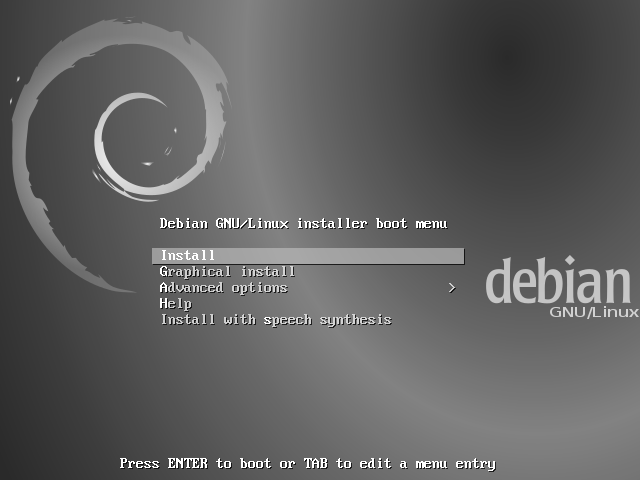
\includegraphics[width=0.8\hsize]{image201509/debian8-inst-01_mono.png}
 \end{center}
 \caption{$B%$%s%9%H!<%i5/F0D>8e(B}
\end{minipage}
 \begin{minipage}{0.5\hsize}
  \begin{center}
   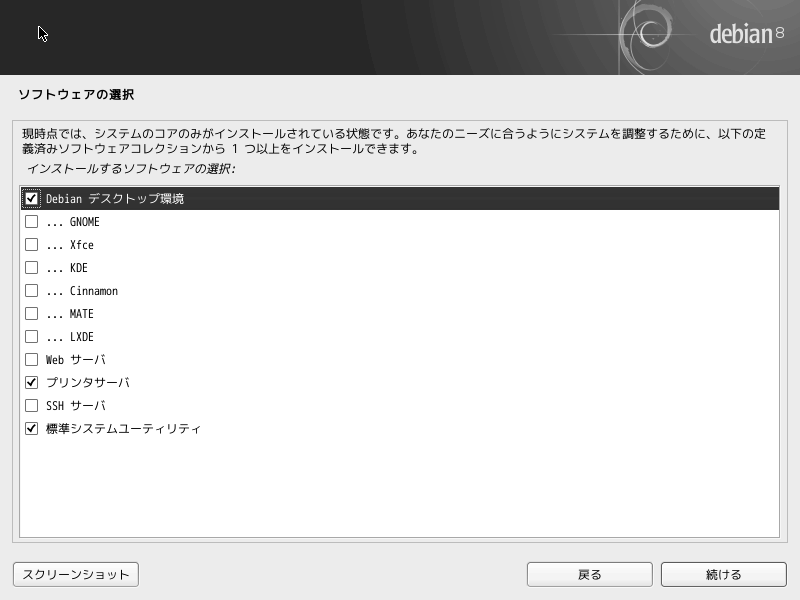
\includegraphics[width=0.8\hsize]{image201509/debian8-inst-02_mono.png}
  \end{center}
  \caption{$B%0%i%U%#%+%k%$%s%9%H!<%k(B}
 \end{minipage}
\end{figure}

\begin{figure}[htbp]
 \begin{minipage}{0.5\hsize}
  \begin{center}
   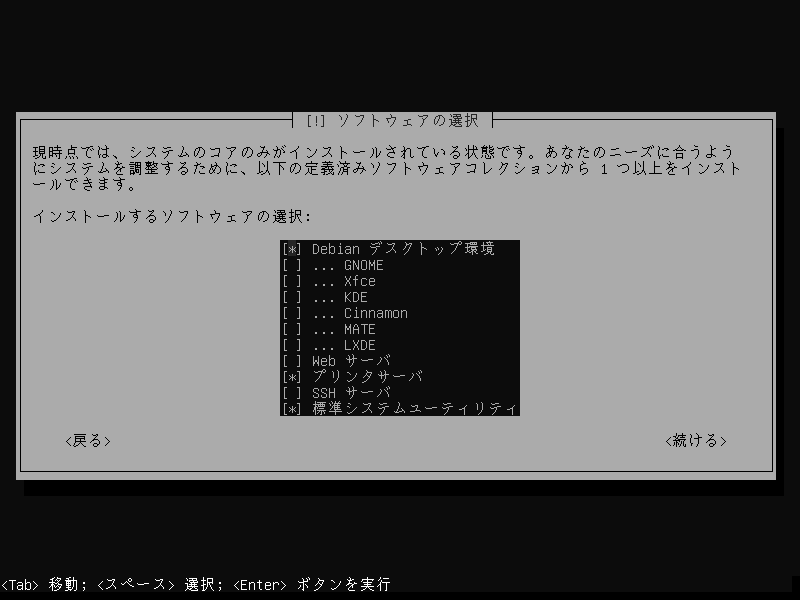
\includegraphics[width=0.8\hsize]{image201509/debian8-inst-03_mono.png}
  \end{center}
  \caption{$B%F%-%9%H%$%s%9%H!<%k(B}
 \end{minipage}
 \begin{minipage}{0.5\hsize}
  \begin{center}
   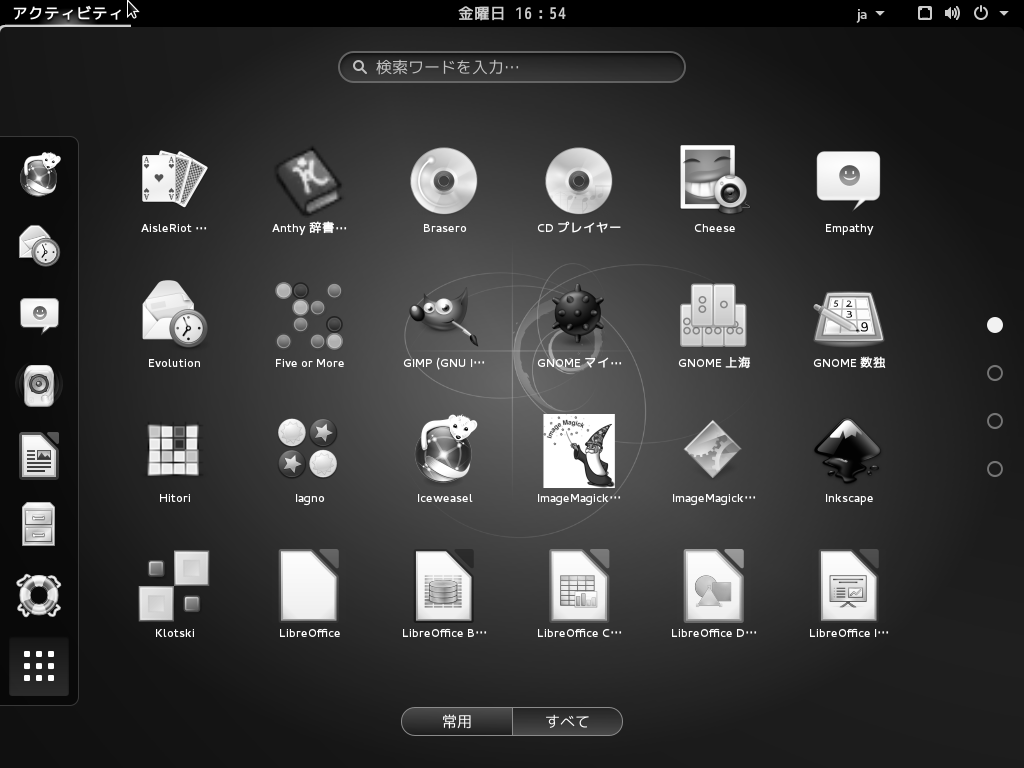
\includegraphics[width=0.8\hsize]{image201509/debian8-gnome_mono.png}
  \end{center}
  \caption{GNOME$B4D6-(B}
 \end{minipage}
\end{figure}

\begin{figure}[htbp]
 \begin{minipage}{0.5\hsize}
  \begin{center}
   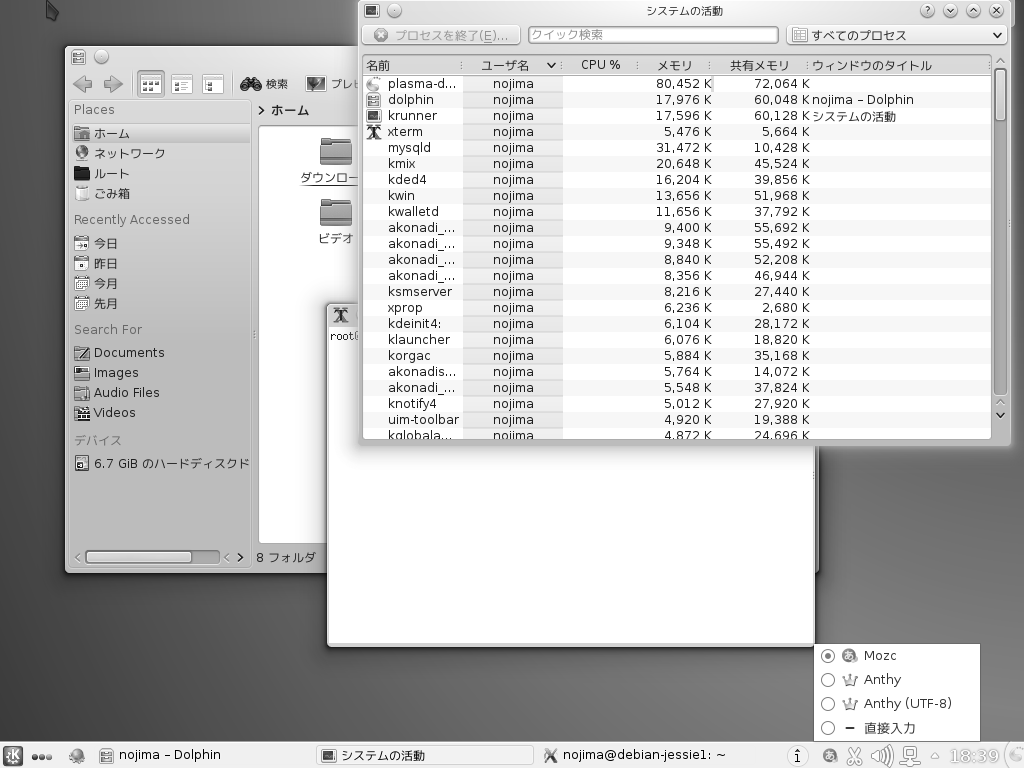
\includegraphics[width=0.8\hsize]{image201509/debian8-kde_mono.png}
   \caption{KDE$B4D6-(B}
  \end{center}
 \end{minipage}
 \begin{minipage}{0.5\hsize}
  \begin{center}
  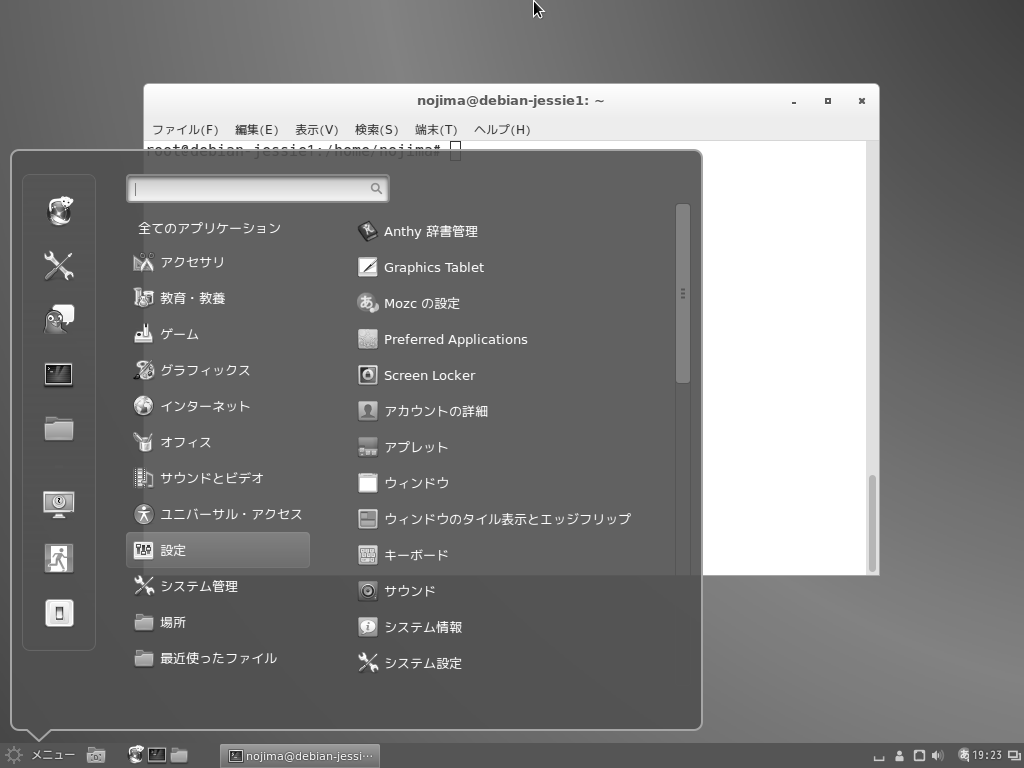
\includegraphics[width=0.8\hsize]{image201509/debian8-cinnamon_mono.png}
  \caption{cinnamon$B4D6-(B}
  \end{center}
 \end{minipage}
\end{figure}

\clearpage

\subsection{$B%j%j!<%9$=$NB>(B}
  \begin{center}
    \Large
2015$BG/(B4$B7n(B30$BF|(B Debian GNU/Hurd 2015$B%j%j!<%9(B
  \end{center}

\begin{itemize}
\item GNU Hurd 0.6$B%Y!<%9(B
\item GNU Mach 1.5$BEk:\(B
\item $B$H$j$"$($:$NF0:n$J$i!"2>A[4D6-$G;n$;$^$9!#@'Hs$*;n$7$"$l!#(B
\end{itemize}


\subsection{Debian GNU/Hurd 2015 Live}

  Live$B%$%a!<%8$b$"$k$h!*(B\\
\url{https://www.gnu.org/software/hurd/hurd/running/debian.html}$B$+$iH4?h(B

\begin{commandline}
# wget http://people.debian.org/~sthibault/hurd-i386/debian-hurd.img.tar.gz
# tar xz < debian-hurd.img.tar.gz
# kvm -m 512 -drive cache=writeback,file=debian-hurd-20150320.img
\end{commandline}
  

\subsection{Debian GNU/Hurd 2015 Live}

Debian GNU/Hurd 2015 Live$B$NMM;R!#(B

\begin{center}
 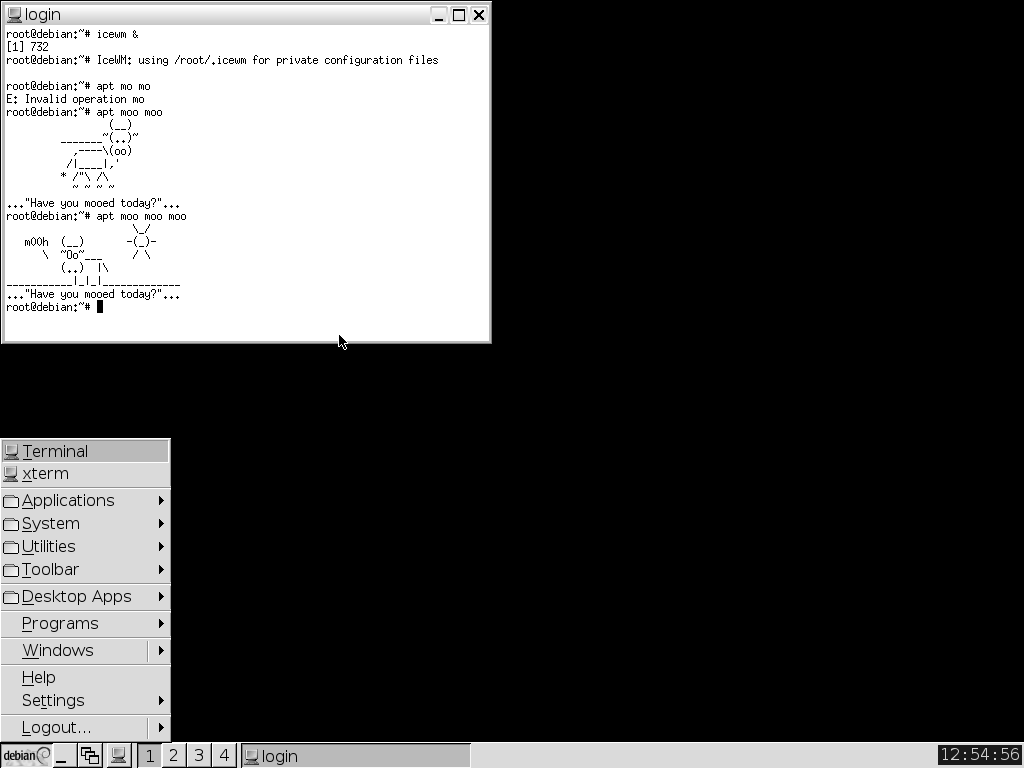
\includegraphics[width=0.9\hsize]{image201509/gnu-hurd-live_mono.png}
\end{center}
 
\subsection{$B<!4|%P!<%8%g%s$N%3!<%IL>(B}

  \begin{itemize}
  \item Debian 9 Stretch $B"+<!2s%j%j!<%9(B
  \item Debian 10 Buster $B"+<!!92s%j%j!<%9(B
  \end{itemize}
  

\subsection{Stretch$B%9%1%8%e!<%k!JM=Dj!K(B}

$B0J2<$O(BStrech$B$N3+H/$K4X$9$kM=Dj!'(B

\begin{itemize}
  \item 2016$BG/(B9$B7n(B5$BF|(B Transition Freeze
  \item 2016$BG/(B11$B7n(B5$BF|(B Soft Freeze
  \item 2016$BG/(B12$B7n(B5$BF|(B Freeze
\end{itemize}

$B;2>H!!(BDebConf15$B$N%j%j!<%9%A!<%`$NF02h!'(B
\url{http://caesar.acc.umu.se/pub/debian-meetings/2015/debconf15/Onwards_to_Stretch_and_other_items_from_the_Release_Team.webm}

 $B$J$*!"(BFreeze$B$O%j%j!<%9$N;v$G$O$J$$$N$GCm0U!#(BStrech$B$KEk:\$9$k?75,$N%Q%C%1!<%8$N<uIU$r40A4$K$d$a!"(BRC$B%P%0DY$7$K@lG0$7$^$9$H$$$&0UL#!#(B
  

\subsection{gcc-5/libc++6 $B0\9T:n6HCf(B}

 $B8=:_!"3+H/HG(B(sid)$B$G$O!"(BStretch$B$K$F?7$7$$%P!<%8%g%s$N%3%s%Q%$%i$G%Q%C%1!<%8$r9=C[$G$-$k$h$&$K$9$k$?$a!"0lC6(Bgcc-5$B7ONs5Z$S!"(Blibc++6$B$N85$G%P%$%J%j%S%k%I$G$-$k$h$&$K$9$kBg:n6H$,9T$o$l$F$$$^$9!#(B

\begin{itemize} 
\item ABI$B%l%Y%k$GJQ99(B
\item C++11$BBP1~(B
\item GFortran$B$G%3%s%Q%$%k$9$k%Q%C%1!<%8$b$3$A$N1F6A$r<u$1$k(B
\end{itemize}


\subsection{httpredir.debian.org$B2TF/3+;O(B}

$B!!%M%C%H%o!<%/4QE@$+$i!"$b$C$H$b6a$$(Bdebian$B$N(Bmirror$B%5%$%H$r>R2p$9$k%5!<%S%9$G$"$C$?!"(B
\begin{itemize}
  \item cdn.debian.net ... DNS$B%/%(%j$G!"$b$C$H$b6a$$(Bmirror$B%5%$%H$rJV$9(B
  \item http.debian.net ... http redirect$B$r;H$C$F!"$b$C$H$b6a$$(Bmirror$B%5%$%H$rJV$9(B
\end{itemize}
$B$,=*N;$7!"Be$o$j$N%5!<%S%9$H$7$F!"@5<0$K(B httpredir.debian.org$B$,2TF/$7$^$7$?!#(B
\\
  $B$,!"$7$+$7K\Mh!"(B
  \begin{commandline}
# cat /etc/apt/souces.list
deb http://httpredir.debian.org/debian/ jessie main
deb-src http://httpredir.debian.org/debian/ jessie main
deb http://httpredir.debian.org/debian/ jessie-updates main
deb-src http://httpredir.debian.org/debian/ jessie-updates main
#
  \end{commandline}
$B$G!"$&$^$/6a$$(Bmirror$B$,>R2p$5$l$k$O$:$,!"2?8N$+F|K\$O@:EY$,0-$$>u67$G$9!#%$%s%9%H!<%i$K$h$C$F@_Dj$5$l$k(Bftp.jp.debian.org$B$NJ}$,8=:_$ONI$$$G$9!#(B

%201506tokyo
%-------------------------------------------------------------------------------
\dancersection{Debian$B$H@H<e@-BP1~$N$"$l$3$l$r$^$H$a$F$_$?(B}{$BLnEg(B $B5.1Q(B}
%-------------------------------------------------------------------------------

\subsection{$B$O$8$a$K(B}

 $B%3%s%T%e!<%?%;%-%e%j%F%#$NJY6/2q$K$FEPCE$rMj$^$l$^$7$?!#$A$g$&$INI$+$C$?$N$G!"(BDebian$B$N@H<e@-BP1~$r$*$5$i$$$7$F!"H/I=$7$F$_$k$3$H$K$7$^$9!#(B

\subsection{Debian$B$N%;%-%e%j%F%#%A!<%`(B}

 Debian$B%Q%C%1!<%8$N@H<e@-LdBj$r@lLg$K07$C$F$$$k?4B!It$N%A!<%`$NO"Mm@h$O0J2<$NDL$j$G$9!#(B

\begin{itemize}
\item security@debian.org $B$^$?$O(B 
\item team@security.debian.org
\end{itemize}

\subsection{$B@H<e@-$K4X$9$k(BML}

 Debian$B$N@H<e@-$K4X$9$k%"%J%&%s%9!&5DO@$,9T$o$l$F$$$k(BML$B$O<!$N$H$*$j$G$9!#(B

 \begin{itemize}
 \item  Debian$B%Q%C%1!<%8$N%;%-%e%j%F%#$K4X$9$k%"%J%&%s%9(B\\
debian-security-announce@lists.debian.org\\
$B%"!<%+%$%V!'(B\\
\url{https://lists.debian.org/debian-security-announce/}
 \item  Debian$B%Q%C%1!<%8$N@H<e@-$K4X$9$k%*!<%W%s$J5DO@(B\\
debian-security@lists.debian.org\\
$B%"!<%+%$%V!'(B\url{https://lists.debian.org/debian-security/}
 \end{itemize}

\subsection{$B@H<e@-BP1~$,9T$o$l$J$$%"!<%+%$%V%(%j%"(B}

$B!!(BDebian$B%Q%C%1!<%872$O!"(Bmain/contrib/non-free$B$N%"!<%+%$%V%(%j%"$G$=$l$>$lDs6!$5$l$F$$$^$9!#<B$O!"@H<e@-BP1~$K$D$$$F!"(Bcontrib/non-free$B$N%"!<%+%$%V%(%j%"$N%Q%C%1!<%8$K$D$$$F$O!"4pK\E*$K=|30$5$l$F$$$^$9!#(B

$B!!$3$A$i$NM}M3$H$7$F$O!"(Bcontrib$B$H(Bnon-free$B$K<}$a$i$l$?%=%U%H%&%'%"$N%i%$%;%s%9$NLdBj$K$h$j$^$9!#$3$l$i$N%=%U%H%&%'%"$O%i%$%;%s%9$NET9g>e!">!<j$KD>$9$3$H$,5vBz$5$l$F$$$J$$>l9g$,$"$k$?$a$H$J$j$^$9!#$b$A$m$s!"(Bcontrib$B$H(Bnon-free$B$G$"$C$F$b!"%i%$%;%s%9>e!"D>$7$F$bNI$$$b$N$b$"$j!"$3$A$i$K$D$$$F$ODL>o$NDL$j%;%-%e%j%F%#%A!<%`$K$F@H<e@-BP1~$,?^$i$l$k$3$H$,$"$j$^$9!#(B

\subsection{$B@H<e@-$K4X$7$F$NBP1~$NN.$l(B}

 Debian$B%f!<%6$"$k$$$O(BDebian$B$N4X78<T$K$+$+$o$i$:!"$b$7@H<e@-$NLdBj$r8+$D$1$?$i!"(B
\begin{description}
\item [PAT1:] $B4{CN$NLdBj(B($B8x3+:Q@H<e@->pJs!K$N>l9g$O!"(Bsecurity$B%?%0$r$D$1$F(BBTS$B$7$F$/$@$5$$!#(B
\item [PAT2:] $B4{CN$G$J$$>l9g$O!"$=$C$H(Bsecurity@debian.org $B$^$?$O(Bteam@security.debian.org $B$K%a!<%k$GO"Mm(B($B1QJ8(B)$B$7!"$"$H$O;X<($K=>$($PNI$$$G$9!#(B
\end{description}

$B!!$b$A$m$s!"@H<e@-BP:v%Q%C%A$b=q$$$?$N$G$"$l$P!"Js9p$N:]$K%Q%C%A$b0l=o$KAw$k$H4n$P$l$^$9!#(B

\subsubsection{$B4{CN$N@H<e@-$G$J$$>l9g$NF0$-(B}

 $B4{CN$N@H<e@-$G$J$$>l9g!"%;%-%e%j%F%#%A!<%`$O(BDebian$B0J30$N%Y%s%@!J%G%#%9%H%j%S%e!<%7%g%sEy4^$`!K4X78<T$i$K$b@H<e@->pJs$,6&M-$5$l!"(BCVE$B$J$I$N@H<e@->pJs%G!<%?%Y!<%9EPO?$K$b6(NO$9$kF0$-$,<h$i$l$^$9!#(B

\subsubsection{$B4{CN$N@H<e@-$N<}=8(B}

$B!!(BMitre$B<R(B(CVE$B$N(BDB$B$r4IM}$7$F$$$k2q<R!K$+$i!"(BCVE$B$N>pJs$rDj4|E*$K<h$j9~$s$G$$$^$9!#$3$A$i$N>pJs$K4p$E$-!"(BDebian$B$K4X78$"$k!&$J$7!"=EMWEY$rH=Dj$7$F;EJ,$1$5$l!"%P%0DI@W%7%9%F%`$KEPO?$7$F$$$/;EAH$_!J%$%s%U%i!K$,$"$j$^$9!#(B

\subsection{$B@H<e@-BP1~>u67$N3NG'J}K!(B}

 $B0J2<$N%5%$%H$G>u67$r3NG'$G$-$^$9!#(B

 \begin{enumerate}
\item $B%;%-%e%j%F%#4QE@$+$i3NG'$7$?$$>l9g(B
  \begin{itemize}
  \item \url{https://security-tracker.debian.org/tracker/}
  \item $BMM!9$J;kE@$+$i!"9+$N@H<e@-%G!<%?%Y!<%9$H(BDebian$B$N3F%Q%C%1!<%8$NBP1~>u67$r3NG'2DG=$G$9!#(B
  \end{itemize}
\item QA$B4QE@$+$i3NG'$7$?$$>l9g(B
  \begin{itemize}
  \item \url{https://tracker.debian.org/}
    $B!!(B\item Debian$B%Q%C%1!<%8$K$D$$$F!"8=:_$N%P%0$N=$@5>u67!"%Q%C%1!<%8$N%j%j!<%9>u67$,%Q%C%1!<%8Kh$K$o$+$j$^$9!#(B
  \end{itemize}
\item BTS$B$7$?!&$5$l$?$b$N$r3NG'$7$?$$>l9g(B
  \begin{itemize}
  \item \url{https://bugs.debian.org/}
  \item BTS$B$7$?7k2L$,$I$&07$o$l$F$$$k$+!"?J9T$7$F$$$k$+3NG'$G$-$^$9!#(B
  \end{itemize}  
\end{enumerate}

 \subsection{$B$=$NB>%H%T%C%/(B}

 $B0J>e$G!"$^$H$a$H$7$F$O=*$o$C$?$N$G!":r:#$N(BDebian$B$N%;%-%e%j%F%#$K4X$9$k%H%T%C%/$r$$$/$D$+>R2p$7$^$9!#(B

 \subsubsection{hardening}

  C/C++$B$G=q$+$l$?%W%m%0%i%`$K$D$$$F!"(Bgcc$B$N5!G=$r3hMQ$7$F!"%;%-%e%j%F%#6/2=$r9T$C$?(BDebian$B%Q%C%1!<%8$r:n$k;n$_$G$9!#(Bhardening$BM-8z;~!"%S%k%I;~$K<B:]$KIU$12C$($i$l$k(Bgcc$B$N%*%W%7%g%s$O0J2<$NDL$j$G$9!#(B
  
\begin{commandline}
-fstack-protector-strong -Wformat -Werror=format-security -D_FORTIFY_SOURCE=2
\end{commandline}

 \subsubsection{Debian$B%Q%C%1!<%8:Q$_$N@H<e@-@EE*2r@O%D!<%k72(B}

  Debian$B$G%Q%C%1!<%8:Q$N@H<e@-@EE*2r@O%D!<%k72$,$"$j$^$9!#(B

\begin{table}
\begin{center}
\begin{tabular}{|c|c|p{5cm}|}
\hline
$B9`HV(B & $B%Q%C%1!<%8L>(B & $B35MW(B \\ \hline \hline
1 & flawfinder & C/C++$B$K$F%;%-%e%j%F%#>eLdBj$N5/$-$=$&$JItJ,$r;XE&!#(B \\ \hline
2 & rats & C, Perl, PHP, Python$B$N%3!<%I>eLdBj$N5/$-$=$&$JItJ,$r;XE&!#(B\\ \hline
3 & pscan & C/C++$B$K$F(Bformat$BJ8$NJ8;zNs$K$D$$$FLdBj$N5/$-$=$&$JItJ,$r;XE&!#(B \\ \hline
\end{tabular}
\end{center}
\caption{Debian$B%Q%C%1!<%8:Q$_@H<e@-@EE*2r@O%D!<%k(B}
\end{table}

\subsubsection{lintian}

 lintian$B$O!"(BDebian$B%Q%C%1!<%8$K$D$$$F!"<+F0$G%9%-%c%s$7$FLdBjE@$r2r@O$7$F7Y9p$7$F$/$l$k%D!<%k$G$"$j!"$"$kDxEY$N%;%-%e%j%F%#BP:v$N0Y$NBP1~$,%Q%C%1!<%83+H/$K$"$?$jI,?\$K$J$C$F$*$j!"$3$A$i$,2aITB-$J$/9T$o$l$F$$$k$+$r%9%-%c%s$7$F3+H/<T$K65$($F$/$l$^$9!#(B

 $B:r:#$K$FEk:\$5$l$?%;%-%e%j%F%$BP1~$NNc$H$7$F!":-Jq$5$l$F$$$k%I%-%e%a%s%H$K(BHTML$B%=!<%9$,$"$C$?>l9g!"30It%j%s%/$,4^$^$l$F$$$k$+$r%9%-%c%s$9$k;v$,DI2C$5$l$^$7$?!#$3$l$O!"$b$7!"%Q%C%1!<%8$K4^$^$l$k%I%-%e%a%s%H$,(BHTML$B$G$"$C$?>l9g$K!"30It%j%s%/$X%"%/%;%9$9$k$h$&$J%?%0$,:.$6$C$F$$$k$h$&$J;v$,L5$$$h$&$K$7$^$9!#$b$7!"$=$&$$$C$?%?%0$d%j%s%/$,;D$C$F$$$k$H!"%I%-%e%a%s%H$r%V%i%&%6$G3+$$$?;~$K!"$&$C$+$j0-0U$N$"$k%5%$%H$X<+F0E*$KM6F3$5$l$F$7$^$&$N$rKI$.$^$9!#(B

\subsubsection{systemd}

 systemd$B$K$O%;%-%e%j%F%#$K4X$7$F6/2=$r?^$k$3$H$,=PMh$k%*%W%7%g%s$,$$$/$D$b$"$j$^$9!#$3$A$i$r$I$&3h$+$7$F!"(Bsystemd$B$N(B*.service$B%U%!%$%k$r:n$k$+$H$$$&$*OC$G$9!#(B
 
$B!!NI$$J8>O$H$7$F!"!V(BSecurity Features in systemd$B!W(B\url{http://0pointer.net/public/systemd-nluug-2014.pdf}$B$,$"$j$^$9$N$G!"8+$F$_$k$H$h$$$G$7$g$&!#(B

\subsubsection{Reproducible Builds}

 Debian$B$N(B22,000$B$rD6$($k%=!<%9%Q%C%1!<%8$r0lC6:F%S%k%I$7!"$9$G$KG[I[$5$l$F$$$k(BDebian$B%Q%C%1!<%8$N%P%$%J%j$H>H9g$9$k;n$_$N;v$G$9!#$3$A$i$K$h$j!"(BDebian$B%Q%C%1!<%8$K$$$D$N4V$K$+0-0U$N$"$k%P%$%J%j$,4^$^$l$F$$$k$h$&$J;v$,L5$$$+$r%A%'%C%/$9$k$N$,A@$$$G$9!#(BDebian$B$NB>$K$b!"(BFedora/OpenSUSE/NixOS$B$G$b9T$o$l$F$$$k$H$N$3$H$G$9!#(B

$B!!>\$7$/$O!"(B
 \begin{description}
\item [Debian]
$B!!!!(B\url{http://reproducible.alioth.debian.org/presentations/2014-02-01-FOSDEM14.pdf}

\item [Fedora]
   \url{http://securityblog.redhat.com/2013/09/18/reproducible-builds-for-fedora/}
 \end{description}

$B$r;2>H$/$@$5$$!#(B
   
\subsubsection{LTS(Long Time Support)}

Debian$B$N3F%P!<%8%g%s$K$D$$$F!"%;%-%e%j%F%#%"%C%W%G!<%H$K$D$$$F$N%5%]!<%H@Z$l$^$G$N4|4V$r(B3$BG/"*(B5$BG/$X1dD9$9$k;n$_$G$9!#C"$7!"?tK|$b$"$k%=%U%H%&%'%"A4It$K$D$$$F(B5$BG/$b%5%]!<%H$9$k$N$OHs8=<BE*$J$N$G!"8B$i$l$?%Q%C%1!<%8$N%;%-%e%j%F%#%"%C%W%G!<%H$N$_1dD9$7$^$9!#(B

\begin{figure}[H]
\begin{center}
 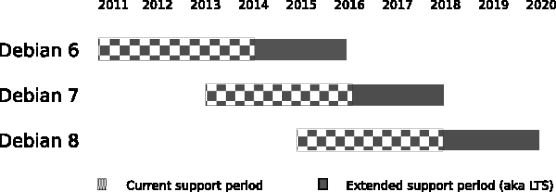
\includegraphics[width=0.7\hsize]{image201506/debian-lts-periods_mono.png}
\end{center}
\caption{LTS$B$N%5%]!<%H4|4V(B}
\end{figure}

 LTS$B$OL5NA$G$bMxMQ$G$-$k0lJ}!"M-=~%5%]!<%H7@Ls$bMQ0U$5$l$F$$$^$9!#(BFreexian$B<R$HM-=~%5%]!<%H7@Ls$r9T$&$N$G$9$,!"J'$C$?CMCJ$K1~$8$F!"%5%]!<%H$7$F$/$l$k%Q%C%1!<%8$NA*Br$NMWK>$,DL$j$d$9$/$J$k$H$$$&FCE5$,$"$k$h$&$G$9!#F|K\$N2q<R$K$F7@LsDy7k<B@S$O(BGREE$B<R$,$"$j$^$9!#(B

 $BM-=~%5%]!<%H7@Ls$K$D$$$F>\$7$/$O!V(BDebian Long Term Support$B!W(B\url{https://www.freexian.com/en/services/debian-lts.html}$B$r;2>H$/$@$5$$!#(B

\subsubsection{debian-security-support$B%Q%C%1!<%8(B}

 debian-security-support$B%Q%C%1!<%8$rF3F~$7!"(Bcheck-support-status$B%3%^%s%I$r<B9T$9$k$H!"(B
$B8=:_$*;H$$$N(BDebian$B5!$KF3F~$5$l$$$F$$$k%Q%C%1!<%8$N@H<e@-$N%5%]!<%H$K$D$$$F!"%5%]!<%H@Z$l!"$b$7$/$O!"2?$i$+$NM}M3$K$h$j@H<e@-BP:v$K$"$?$j@)8B$r2C$($6$k$rF@$J$+$C$?$b$N$N%j%9%H$,<h$l$k$h$&$K$J$j$^$7$?!#(B

$B!!$3$N%3%^%s%I$NF0:n$H$7$F$O!"(B
\begin{itemize}
\item  /usr/share/debian-security-support/security-support-ended
\item /usr/share/debian-security-support/security-support-limited
\end{itemize}
$B$K5-:\$5$l$?%Q%C%1!<%8$N%5%]!<%H>u67$K4X$9$k@)8B$N>pJs$H!"<B:]$KF3F~$5$l$F$$$F$k%Q%C%1!<%8L>$r>H9g$9$k$3$H$K$h$jF0:n$7$^$9!#$b$7!"$3$l$i$N%U%!%$%k$+$i!"@)8B$,$"$k%Q%C%1!<%8$,%^%7%s$K8+$D$+$C$?>l9g$O!"7Y9p$r=P$7$F$/$l$^$9!#$J$*!"(BLTS$B$G$O!"$I$3$^$G%Q%C%1!<%8$K$D$$$F!"@H<e@-BP1~$N%5%]!<%H$,$J$5$l$F$$$k$+$N3NG'$,$G$-$^$9!#(B

\subsection{$B$*$o$j$K(B}

$B!!(BDebian$B$N@H<e@-BP1~$K$D$$$F$^$H$a$F$_$^$7$?!#(BDebian$B$N%;%-%e%j%F%#0];}$N0Y!"MM!9$JEXNO$,J'$o$l$F$$$k$3$H$,$o$+$j$^$7$?!#(B

%201511 tokyo
%-------------------------------------------------------------------------------
\dancersection{Debian GNU/kFreeBSD $B%;%C%H%"%C%W%,%$%I(B 2015$BG/HG(B}{$B?yK\(B $BE5=<(B}
%-------------------------------------------------------------------------------

\subsection{$B$O$8$a$K(B}

Debian GNU/kFreeBSD$B$O!"(BFreeBSD$B%+!<%M%k$GF0:n$9$k(BDebian$B$G$9!#(BDebian$B$OC1$J$k(BLinux$B%G%#%9%H%j%S%e!<%7%g%s$G$O$J$/!"%f%K%P!<%5%k%*%Z%l!<%F%#%s%0%7%9%F%`$rL\;X$7$F$*$j!"$=$NNc$H$7$F(BDebian GNU/kFreeBSD$B$,$"$j$^$9!#(B\footnote{$B;d$,CN$C$F$$$k8B$j!V(BUniversal Operating System$B!W$H$$$&5-=R$OK\2H(Bweb$B%5%$%H%H%C%W%Z!<%8$N(Btitle$B%?%0$G$7$+8+$?$3$H$J$$$G$9!#(B}

$B$?$@(BDebian GNU/kFreeBSD$B$O$=$NFC0[$5$f$($K(BDebian GNU/Linux$B$H0[$J$kE@$,$"$j$^$9!#:#2s$O!"(BDebian GNU/kFreeBSD$B$K?($l$k$K$"$?$j!"$I$N$h$&$K%;%C%H%"%C%W$r9T$&$H$h$$$+@bL@$7$^$9!#(B

\subsection{Debian Ports$B$H(BDebian GNU/kFreeBSD}

Debian Ports\footnote{\url{https://www.debian.org/ports/}}$B$H$O!"$5$^$6$^$J(BCPU$B$d%+!<%M%k$GF0:n$9$k$h$&$K0\?"$r9T$&%W%m%8%'%/%H$N$3$H$G$9!#(B

FreeBSD$B%+!<%M%k$G5/F0$9$k(BDebian$B$r:n$k%W%m%8%'%/%H$,$"$j!"$=$N(BDebian$B$N$3$H$r!V(BDebian GNU/kFreeBSD$B!W$H8F$s$G$$$^$9(B(k$B$O(Bkernel$B$N$3$H(B)$B!#8=:_$G$O(BIntel CPU$B$N%"!<%-%F%/%A%c$N$_$"$j$^$9(B(kfreebsd-amd64$B!"(Bkfreebsd-i386)$B!#(BDebian 6 (Squeeze)$B$G$O%F%/%N%m%8!<%W%l%S%e!<$H$7$F=i$a$F(Bstable$B%j%j!<%9$5$l$^$7$?!#(BDebian 7 (Wheezy)$B$G$b7QB3$7$F(Bstable$B%j%j!<%9$5$l$?$N$G$9$,!"(BDebian 8 (Jessie)$B$G$O(BDrop$B$H$J$C$?$?$a%j%j!<%9$5$l$F$$$^$;$s!#(B\footnote{\url{https://lists.debian.org/debian-devel-announce/2014/09/msg00002.html} $B$K$*$$$F!"(Bstable$B$r0];}$7$D$D(Bsid$B$N3+H/$r?J$a$k$K$O$=$l$J$j$K?M<j$,I,MW$G$"$k$,!"(BkFreeBSD$B$r:n6H$9$k?M<j$OITB-$7$F$$$k$3$H$,;XE&$5$l$F$$$^$9!#(B}


\subsection{Debian GNU/kFreeBSD$B$N%$%s%9%H!<%k(B}
\subsubsection{$B%$%s%9%H!<%k%$%a!<%8$NF~<j(B}

\url{https://www.debian.org/devel/debian-installer/}$B$K$"$k(Bdaily-images$B$r;H$C$F%$%s%9%H!<%k$7$^$9!#(B
kfreebsd-amd64$BHG$N(Bmini.iso$B$r%@%&%s%m!<%I$7!"(BUSB$B%a%b%j$K(Bdd$B$7$F%$%s%9%H!<%k%G%#%9%/$r:n@.$7$^$9!#(Bkfreebsd-i386$BHG$N(Bmini.iso$B$rMxMQ$7$F$b9=$o$J$$$N$G$9$,!"%U%!%$%k%7%9%F%`$K(BZFS$B$r;H$&>l9g$O%a%b%jITB-$K$J$j$,$A$J$?$aCm0U$7$F$/$@$5$$!#(B

mini.iso$B$r(Bdd$B$7$?(BUSB$B%a%b%j$r:9$7$F(BPC$B$r5/F0$9$k$H(BDebian Installer$B$,5/F0$7$^$9!#$J$*!"8=;~E@$N(Bkfreebsd$BHG(BDebian Installer$B$O0J2<$N@)Ls$,$"$j$^$9!#(B\footnote{$BK\2H(BFreeBSD-10.1$B$N%$%s%9%H!<%i$O(BUEFI$B%V!<%H$KBP1~$7!"%G%#%9%/7A<0$r(BGPT$B$H$7$F%$%s%9%H!<%k$9$k$3$H$,2DG=$G$9!#(B}
\begin{itemize}
  \item UEFI$B%V!<%H$KBP1~$7$F$$$J$$(B
  \item $B%G%#%9%/7A<0$O(BMBR$B$N$_$KBP1~$7$F$$$k(B(GPT$B$OHsBP1~(B)
\end{itemize}


\subsubsection{$B%$%s%9%H!<%i$NI=<(8@8l(B}

kfreebsd$BHG(BDebian Installer$B$O!"F|K\8l$NI=<($,$G$-$^$;$s(B($B%$%s%9%H!<%i$G%U%l!<%`%P%C%U%!$,M-8z$K$J$C$F$$$J$$$H;W$o$l$k(B)$B!#$=$N$?$a!"(BLANG=C$B$G%$%s%9%H!<%k$r?J$a$^$9!#(B

\subsubsection{$B%Q!<%F%#%7%g%s9=@.$H%U%!%$%k%7%9%F%`(B}

Debian GNU/kFreeBSD$B$r%$%s%9%H!<%k$9$k$H$-$O(Broot$B%Q!<%F%#%7%g%s$r(BMBR$B$N4pK\%Q!<%F%#%7%g%s$K$9$kI,MW$,$"$j$^$9!J3HD%%Q!<%F%#%7%g%s$K%$%s%9%H!<%k$9$k$H(Bgrub$B$N%$%s%9%H!<%k$K<:GT$7$^$9!K!#(Bswap$B%Q!<%F%#%7%g%s$O3HD%%Q!<%F%#%7%g%s$K:n@.$7$F$bLdBj$"$j$^$;$s!#(B

$B$3$NA0Ds$,$"$k$?$a!"%W%j%$%s%9%H!<%k$N(BWindows$B$H%G%e%"%k%V!<%H$7$?$$>l9g$O!"0J2<$N%Q!<%F%#%7%g%s9=@.$G$[$\7h$^$j$K$J$j$^$9!#(B\footnote{$B%U%!%$%k%7%9%F%`$r(BUFS$B$K$9$k>l9g$O4pK\%Q!<%F%#%7%g%s$N>e8B(B($B#4$D(B)$B$rD6$($k$3$H$,$"$k$?$a!"%G%#%9%/Fb$N(BWindows$BMQ%j%+%P%jNN0h$r:o=|$9$k!"(BD$B%I%i%$%V$r:o=|$9$k$J$I$N;vA0=`Hw$,I,MW$K$J$j$^$9!#(B}

\begin{commandline}
# fdisk -l /dev/ada0
Disk /dev/ada0: 298.1 GiB, 320072933376 bytes, 625142448 sectors
Units: sectors of 1 * 512 = 512 bytes
Sector size (logical/physical): 512 bytes / 512 bytes
I/O size (minimum/optimal): 512 bytes / 512 bytes
Disklabel type: dos
Disk identifier: 0x33d61950

Device      Boot     Start       End   Sectors   Size Id Type
/dev/ada0p1 *         2048   2459647   2457600   1.2G  7 HPFS/NTFS/exFAT
  -> Windows 7$B$N%$%s%9%H!<%i$,<+F0$G3NJ]$9$kNN0h(B
/dev/ada0p2        2459648 375142399 372682752 177.7G  7 HPFS/NTFS/exFA
  -> Windows 7$B$N(BOS$B$r%$%s%9%H!<%k$7$?(BNTFS$B%Q!<%F%#%7%g%s(B
/dev/ada0p3      580083712 625140399  45056688  21.5G  7 HPFS/NTFS/exFAT
  -> $B%N!<%H(BPC$B%a!<%+!<$N%j%+%P%j!<NN0h(B
/dev/ada0p4      375142400 580083711 204941312  97.7G a5 FreeBSD
  -> Debian GNU/kFreeBSD$B$r%$%s%9%H!<%k$9$k(BZFS$B%9%H%l!<%8%W!<%kNN0h(B
  -> ZFS$B%Q!<%F%#%7%g%s$NCf$K(Broot$B%\%j%e!<%`$H(Bswap$B%\%j%e!<%`$r:n@.$7$^$9(B
\end{commandline}

4$B$D$N4pK\%Q!<%F%#%7%g%s$K$&$A!"(B1$B$D$r(BZFS$B%9%H%l!<%8%W!<%k(B(LVM$B$NJ*M}%\%j%e!<%`$K;w$F$$$k35G0(B)$B$K3d$jEv$F$^$9!#$=$7$F(BZFS$B%9%H%l!<%8%W!<%k$+$i(Broot$B%\%j%e!<%`$H(Bswap$B%\%j%e!<%`$r:n@.$7$^$9(B($BJLES(Bboot$B%\%j%e!<%`$r:n@.$7$F(B/boot$B%Q!<%F%#%7%g%s$X3d$jEv$F$7$J$/$F$bLdBj$"$j$^$;$s(B)$B!#(B

$B%G%#%9%/$9$Y$F$r(Bkfreebsd$B$K3d$jEv$F$k$3$H$,$G$-!"$+$D%a%b%jEk:\NL$,>/$J$$4D6-(B($B8E$$(BPC$B$d2>A[%^%7%s(B)$B$X%$%s%9%H!<%k$9$k>l9g$O(BUFS$B$rA*Br$7$?$[$&$,$h$$$H;W$$$^$9!#(B\footnote{$B%$%s%9%H!<%k;~$K:n@.$9$k(BUFS$B%Q!<%F%#%7%g%s$O(Bsoft update$B$,L58z$K$J$C$F$$$^$9(B($B$D$^$jF14|=q$-9~$_$9$k@_Dj$K$J$C$F$$$k(B)$B!#(Brescue mode$B$+$i(B"tunefs.ufs -n enable "partition-path""$B$r<B9T$9$k$H(Bsoft update$B$rM-8z$K$7$FHsF14|=q$-9~$_$KJQ99$G$-$^$9$,!"BQ>c32@-$,Dc2<$7$^$9$N$G$4Cm0U$/$@$5$$!#(B}

\subsection{Debian GNU/kFreeBSD$B8GM-$N(BDebian$B%Q%C%1!<%8(B}

Debian GNU/kFreeBSD$B8GM-$N%Q%C%1!<%8$NNc$r>R2p$7$^$9!#(B

\subsubsection{kfreebsd-image$B%Q%C%1!<%8(B}

Debian GNU/kFreeBSD$B$N(Bkernel$B%$%a!<%8$r<}O?$7$?%Q%C%1!<%8$G$9!#(Bunstable$B$K$O(Bkfreebsd-image-10.1$B$,$"$j8=>u$N%G%U%)%k%H(Bkernel$B$K$J$C$F$$$^$9!#(Bexperimental$B$K$O(Bkfreebsd-image-10.2\footnote{FreeBSD-10.2$B$O(B2015$BG/(B8$B7n(B14$BF|(B UTC$B$K%j%j!<%9$5$l$F$$$^$9$N$G<!Bh$K$3$A$i$,%G%U%)%k%H$K$J$k$G$7$g$&!#(B}$B!"(Bkfreebsd-image-11\footnote{$B8=:_$N(BFreeBSD-CURRENT$B$G$9!#(BFreeBSD-CURRENT$B$O!"(Bdebian$B$G$$$&$H$3$m$N(Bunstable$B$H;w$?0LCVIU$1$G$"$j!":G?7$N3+H/HG$G$9!#(B}$B$b$"$j$^$9!#(B

\subsubsection{zfsutils$B%Q%C%1!<%8(B}

zfsutils$B%Q%C%1!<%8$O(BZFS$B$rA`:n$9$k%3%^%s%I$r4^$s$@%Q%C%1!<%8$G$9!#%$%s%9%H!<%k;~$N%U%!%$%k%7%9%F%`$K(BZFS$B$rA*Br$7$?>l9g$O%G%U%)%k%H$G%$%s%9%H!<%k$5$l$^$9!#(B

kfreebsd-image-10.1$B$GMxMQ$G$-$k(BZFS$B$N%P!<%8%g%s$O(Bver 28$B$H$J$C$F$$$^$9!#(B

\begin{commandline}
  $ zpool upgrade -v
  (snip)
  28  Multiple vdev replacements
\end{commandline}

\subsubsection{freebsd-utils$B%Q%C%1!<%8(B}

FreeBSD$B8GM-$N%3%^%s%I$r4^$s$@%Q%C%1!<%8$G$9!#(B/sbin/mount\_*$B!"(B/usr/sbin/jail$B$J$I$,F~$C$F$$$^$9!#(B

\subsubsection{freebsd-smbfs$B%Q%C%1!<%8(B}

freebsd-smbfs$B%Q%C%1!<%8$O!"(BWindows$B%U%!%$%k6&M-(B(SMB$B6&M-(B)$B$X%"%/%;%9$9$k$?$a$N%Q%C%1!<%8$G$9!#(B
$B%$%s%9%H!<%k$9$k$H!"(B/usr/sbin/mount\_smbfs$B%3%^%s%I$,;H$($k$h$&$K$J$j$^$9!#(B

Windows$B%U%!%$%k6&M-@h$r(Bmount$B$9$k$K$O0J2<$N%3%^%s%I$r<B9T$7$^$9!#(B

\begin{commandline}
# mount_smbfs -E UTF-8:CP932 -I {$B%U%!%$%k%5!<%P$N(BIP$B%"%I%l%9(B} -U {smb$B%f!<%6L>(B} //{$B%U%!%$%k%5!<%P$N(BIP$B%"%I%l%9(B}/{dir} {mount$B@h(Bdir}
\end{commandline}

\subsubsection{freebsd-ppp$B%Q%C%1!<%8(B}

freebsd-ppp$B%Q%C%1!<%8$O!"%@%$%"%k%"%C%W$9$k(B/usr/sbin/ppp$B%3%^%s%I$r4^$s$G$$$^$9!#(B3G$B$d(BLTE$B$KBP1~$7$?(BUSB$B%b%G%`$r;H$&>l9g$KI,MW$H$J$j$^$9!#(B

Debian GNU/Linux$B$G$O(Bppp$B%Q%C%1!<%8$d(Bwvdial$B%Q%C%1!<%8$G%@%$%"%k%"%C%W$7$^$9$,!"(Bkfreebsd$B$G$O;H$($J$$$?$aCm0U$,I,MW$G$9!#(B

ppp$B@\B3$NNc$K$D$$$F$O8e=R$7$^$9!#(B

\subsubsection{pf$B%Q%C%1!<%8(B}

FreeBSD kernel$B$,$b$D(BPacket Filter$B$H8F$P$l$k$$$o$f$k%U%!%$%"%&%)!<%k5!G=$r@)8f$9$k%3%^%s%I(B/sbin/pfctl$B$r4^$s$@%Q%C%1!<%8$G$9!#(B\footnote{Linux kernel$B$N(Bnetfilter$B5!G=$H@)8f%3%^%s%I(Biptables$B$KAjEv$7$^$9!#(B}

/sbin/pfctl$B$N@_Dj%U%!%$%k$O(B/etc/pf.conf$B$G$"$j!"(BLinux$B$N(Biptables$BMQ@_Dj%U%!%$%k$HCf?H$,A4$/0[$J$j$^$9!#(B

\subsection{Windows$B$H(BDebian GNU/kFreeBSD$B$N%G%e%"%k%V!<%H@_Dj(B}

Debian GNU/kFreeBSD$B$N(Bboot loader$B$O(Bgrub2$B$rMxMQ$7$F$$$^$9!#(B
grub2$B$G(BDebian GNU/kFreeBSD$B$H(BWindows$B$r%G%e%"%k%V!<%H$7$?$$>l9g$O0J2<$NA`:n$r9T$$!"(Bgrub$B$K%a%K%e!<$rDI2C$7$^$9!#(B((hd0,2)$B$NItJ,$O%$%s%9%H!<%k4D6-$K9g$o$;$FJQ99$7$F$/$@$5$$(B))

\begin{commandline}
  # cd /etc/grub
  # vi 40_custom.kfreebsd
  
  #!/bin/sh
  exec tail -n +3 $0
  # This file provides an easy way to add custom menu entries.  Simply type the
  # menu entries you want to add after this comment.  Be careful not to change
  # the 'exec tail' line above.
  menuentry ``Windows (loader)'' {
    insmod part_msdos
    insmod ntfs
    set root=(hd0,2)
    chainloader +1
  }

  # update-grub
\end{commandline}

\subsection{$B%O!<%I%&%'%"$H%=%U%H%&%'%"$N%;%C%H%"%C%W(B}
\subsubsection{$BM-@~(BLAN}

$BM-@~(BLAN$B$OMxMQ$9$k%I%i%$%P$K$h$C$F%G%P%$%9L>$,JQ2=$7$^$9(B(intel$B$N(BPC$B8~$1$J$i(Bem0$B!"(Brealtek$B$J$i(Bre0)$B!#(B
$B@_Dj%U%!%$%k$O(BDebian GNU/Linux$B$HF1$8(B/etc/network/interfaces$B$G$9$,!"(Ballow-hotplug$B6g$O(Blinux$B$G;H$o$l$k(Budev$B$,Ds6!$7$F$$$k5!G=$G$"$k$3$H$+$i(Bkfreebsd$B$G$OMxMQ$G$-$J$$$?$aCm0U$,I,MW$G$9!#(B

$B$=$N$?$a!"M-@~(BLAN$B@\B34D6-$,$J$$>u67$G(BOS$B$r5/F0$9$k$HM-@~(BLAN$B$K$h$k(BDHCP$B$N(BIP$B%"%I%l%9<hF@$,%?%$%`%"%&%H$9$k$^$G(Blogin$B%W%m%s%W%H$,=P$F$3$J$/$J$j$^$9(B($B5/F0$K;~4V$,$+$+$k(B)$B!#;d$O%N!<%H(BPC$B$K(BDebian GNU/kFreeBSD$B$r%$%s%9%H!<%k$9$k>l9g$O0J2<%3%^%s%I$r<jF0$G<B9T$7$F%M%C%H%o!<%/$X@\B3$9$k$h$&$K$7$F$$$^$9!#(B

\begin{commandline}
  # vi /etc/network/interfaces

  #auto em0  <-$B%3%a%s%H$K$7$^$9(B
  iface lan_home inet dhcp

  
  # ifup em0=lan_home
\end{commandline}

\subsubsection{$BL5@~(BLAN}

$BL5@~(BLAN$B$O(BThinkpad X220$B$KEk:\$7$F$$$k!V(BIntel Centrino advanced-N 6205$B!W$GF0:n$9$k$3$H$r3NG'$7$F$$$^$9!#$=$N$?$a!"F1$8(Biwn$B%G%P%$%9$HG'<1$5$l$k!V(BIntel Wireless WiFi Link 4965$B!W0J9_$N(BIntel$B@=L5@~(BLAN$B%+!<%I$G$"$l$PF0:n$9$k$H;W$$$^$9!#(B

$BL5@~(BLAN$B$rMxMQ$9$k$?$a$K(Bkfreebsd-image-10$B7O$N:G?7HG(Bkernel$B!"(Bfirmware$B!"L5@~(BLAN$B%G!<%b%s(B"wpasupplicant"$B$r%$%s%9%H!<%k$7$^$9!#(B\footnote{kfreebsd$B$GL5@~(BLAN$B$,;H$($k$h$&$K$J$C$?$N$O(B2014$BG/(B8$B7n:"$H;W$o$l$^$9!#(B \url{https://bugs.debian.org/cgi-bin/bugreport.cgi?bug=642468}}

\begin{commandline}
  # vi /etc/apt/sources.list

  deb http://ftp.jp.debian.org/debian/ unstable main contrib non-free

  # apt-get install kfreebsd-image-10-amd64
  # apt-get install firmware-iwlwifi wpasupplicant
  # reboot
\end{commandline}

FreeBSD$B$NL5@~(BLAN$B%$%s%?%U%'!<%9$O!"J*M}%$%s%?%U%'!<%9$HO@M}%$%s%?%U%'!<%9$KJ,$+$l$F$$$^$9!#$=$N$?$a!"O@M}%$%s%?%U%'!<%9$r@8@.$9$kI,MW$,$"$j$^$9!#(B

\begin{commandline}
  # ifconfig iwn0  ($B$3$l$,J*M}%$%s%?%U%'!<%9L>(B)
  iwn0: flags=8802 metric 0 mtu 2290
  ether xx:xx:xx:xx:xx:xx
  media: IEEE 802.11 Wireless Ethernet autoselect (autoselect)
  status: no carrier
  nd6 options=23

  # ifconfig wlan create wlandev iwn0
  wlan0

  # ifconfig wlan0 ($B$3$l$,O@M}%$%s%?%U%'!<%9L>(B)
  wlan0: flags=8802 metric 0 mtu 1500
  ether xx:xx:xx:xx:xx:xx
  inet6 fe80::xxxx:xxxx:xxxx:xxxx%wlan0 prefixlen 64 scopeid 0x6
  ssid " channel 5 (2432 MHz 11g)
  country US authmode WPA2/802.11i privacy OFF txpower 15 bmiss 10
  scanvalid 60 bgscan bgscanintvl 300 bgscanidle 250 roam:rssi 7
  roam:rate 5 protmode CTS wme
  media: IEEE 802.11 Wireless Ethernet autoselect (autoselect)
  status: no carrier
      nd6 options=23
\end{commandline}
%" -- for emacs

$B@\B3$9$kL5@~(BLAN$B%"%/%;%9%]%$%s%H$NG'>Z>pJs@_Dj%U%!%$%k$r:n@.$7$^$9!#(B

\begin{commandline}
  $ wpa_passphrase apname1 appassword > wpa_apname1.conf
  $ cat wpa_apname1.conf
  network={
    ssid=''apname1''
    #psk=''appassword''
    psk=e9fdcb43eba09b6342df30f14275625c8494e534799a82d6639b6124434ea627
  }  
\end{commandline}

$BL5@~(BLAN$B%"%/%;%9%]%$%s%H$X@\B3$7!"(BDHCP$B$G(BIP$B%"%I%l%9$r<hF@$7$^$9!#(BIP$B%"%I%l%9$OO@M}%$%s%?%U%'!<%9$KIUM?$5$l$^$9!#(B

\begin{commandline}
  # wpa_supplicant -i wlan0 -c ./wpa_apname1.conf
  Successfully initialized wpa_supplicant
  ioctl[SIOCS80211, op=20, val=0, arg_len=7]: Invalid argument
  ioctl[SIOCS80211, op=20, val=0, arg_len=7]: Invalid argument
  wlan0: Trying to associate with yy:yy:yy:yy:tt:tt (SSID='apname1' freq=2432 MHz)
  wlan0: Associated with yy:yy:yy:yy:yy:yy
  wlan0: WPA: Key negotiation completed with yy:yy:yy:yy:yy:yy [PTK=CCMP GTK=CCMP]
  wlan0: CTRL-EVENT-CONNECTED - Connection to yy:yy:yy:yy:yy:yy completed [id=0 id_str=]
  wlan0: WPA: Group rekeying completed with yy:yy:yy:yy:yy:yy [GTK=CCMP]

  # dhclient wlan0

  # /sbin/ifconfig wlan0
  wlan0: flags=8843 metric 0 mtu 1500
  ether xx:xx:xx:xx:xx:xx
  inet6 fe80::xxxx:xxxx:xxxx:xxxx%wlan0 prefixlen 64 scopeid 0x6
  inet 192.168.1.100 netmask 0xffffff00 broadcast 192.168.1.255
  ssid apname1 channel 5 (2432 MHz 11g) bssid yy:yy:yy:yy:yy:yy
  country US authmode WPA2/802.11i privacy ON deftxkey UNDEF
  AES-CCM 2:128-bit txpower 15 bmiss 10 scanvalid 60 bgscan
  bgscanintvl 300 bgscanidle 250 roam:rssi 7 roam:rate 5 protmode CTS
  wme roaming MANUAL
  media: IEEE 802.11 Wireless Ethernet OFDM/48Mbps mode 11g
  status: associated
          nd6 options=23
\end{commandline}

wpasupplicant$B%3%^%s%I$GL5@~(BLAN$B%"%/%;%9%]%$%s%H$X@\B3$r;n$_$?$,%(%i!<$,H/@8$7@\B3$G$-$J$$>l9g$,$"$j$^$9!#$=$N>l9g$O0J2<$r;n$9$H@\B3$G$-$k>l9g$,$"$j$^$9!#(B

\begin{itemize}
  \item $B@\B3@h(BSSID$B$r(B2.4GHz$BBS$N$b$N$KJQ99$9$k!#(B
  \item ``\texttt{\# ifconfig wlan0 -ht40}'' $B$r<B9T$9$k!#(B\footnote{$B%G%e%"%k%A%c%M%k@\B3$rL58z$K$7$F!"(B20MHz$BI}$NEEGH$GDL?.$9$k$h$&$K;X<($9$k%3%^%s%I$G$9!#(B}
\end{itemize}


\subsubsection{USB$B%b%G%`$K$h$k%@%$%"%k%"%C%W(B}

3G$B$d(BLTE$B$N(BUSB$B%b%G%`$r;H$C$F%@%$%"%k%"%C%W@\B3$9$k$3$H$,$G$-$^$9!#(BNTT$B%I%3%b$+$i=P$F$$$k!V(BL-02C$B!W$H$$$&(BLTE$B$KBP1~$7$?(BUSB$B%b%G%`$rNc$K@\B3$9$k<j=g$r@bL@$7$^$9!#(B

$B$^$:$O(Bppp$B%3%^%s%I$H(BUSB$B%b%G%`=hM}$K;H$&%3%^%s%I$r%$%s%9%H!<%k$7$^$9!#(B

\begin{commandline}
  # apt-get install freebsd-ppp usb-modeswitch 
\end{commandline}

L-02C$B$r(BPC$B$K:9$9$H(BCD-ROM$B%G%P%$%9$H$7$FG'<1$7$^$9!#$=$N$?$a!"(BL-02C$B$r%b%G%`%b!<%I$KJQ99$9$k%3%^%s%I$r<B9T$7$^$9!#(B

\begin{commandline}
  # vi /etc/usb_modeswitch.d/L02C.conf
  ########################################################
  # LG L-02C LTE modem

  DefaultVendor= 0x1004
  DefaultProduct=0x61dd

  TargetVendor= 0x1004
  TargetProduct=0x618f

  MessageContent=5553424312345678000000000000061b000000020000000000000000000000
  NeedResponse=1
  CheckSuccess=20

  # usb_modeswitch -c /etc/usb_modeswitch.d/L02C.conf
\end{commandline}

\begin{commandline}
  # ls /dev/cua*
  /dev/cuaU0.0       /dev/cuaU0.1       /dev/cuaU0.2       /dev/cuaU0.3
  /dev/cuaU0.0.init  /dev/cuaU0.1.init  /dev/cuaU0.2.init  /dev/cuaU0.3.init
  /dev/cuaU0.0.lock  /dev/cuaU0.1.lock  /dev/cuaU0.2.lock  /dev/cuaU0.3.lock
\end{commandline}

$B<!$K(Bppp$B%3%^%s%I$N@_Dj%U%!%$%k$r:n@.$7!"(Bppp$B@\B3$7$^$9!#MxMQ$9$k2s@~$K$h$C$FE,;~(BAPN$B!"%f!<%6L>!"%Q%9%o!<%I$OJQ99$7$F$/$@$5$$!#(BPPP$B@\B3$K@.8y$9$k$H(Btun$B%$%s%?%U%'!<%9$,@8@.$5$l!"(BIP$B%"%I%l%9$,IUM?$5$l$^$9!#(B

\begin{commandline}
  # vi /etc/ppp/ppp.conf

  default:
    set log Phase Chat LCP IPCP CCP tun command
    ident user-ppp VERSION
    set device /dev/cuaU0.2
    set speed 38400
    set dial ``ABORT BUSY TIMEOUT 2 \
    \"\" \
    AT OK-AT-OK \
    AT+CFUN=1 OK-AT-OK \
    AT+CMEE=2 OK-AT-OK \
    AT+CSQ OK \
    AT+CGDCONT=1,\\\"IP\\\",\\\"apn.ne.jp\\\" OK \
    AT+CGACT? OK-AT-OK \
    AT+CGATT? OK \
    AT+CGCLASS? OK \
    AT+COPS? OK \
    ATD*99***1# CONNECT''
    set timeout 180
    enable dns

  myppp:
    set phone ``*99***1#''
    set authname ``apnuser''
    set authkey ``apnpass''
    set timeout 300
    disable ipv6
    set ifaddr 10.1.0.1/0 10.1.0.2/0 255.255.255.255 0.0.0.0
    add default HISADDR

  # ppp -foreground myppp
\end{commandline}

\subsubsection{$B%S%G%*%I%i%$%P(B}

$B8=:_!"<gN.$N%S%G%*%+!<%I$O(BIntel$B<R$N(BCPU$BFbB"%0%i%U%#%C%/%9!"(BAMD$B<R$N(BRadeon$B%7%j!<%:!"(BNVIDIA$B<R$N(BGeForce$B%7%j!<%:$,$"$j$^$9!#(B
Debian GNU/kFreeBSD$B$O(BFreeBSD$B8~$1$KDs6!$5$l$k%W%m%W%i%(%?%j%I%i%$%P$N%S%k%I4D6-$,$J$$$?$a!"%*!<%W%s%=!<%9HG%I%i%$%P$rMxMQ$9$kI,MW$,$"$j$^$9!#$=$N$?$a!"(BIntel CPU$BFbB"%0%i%U%#%C%/%9$^$?$O(BRadeon$B%7%j!<%:$N%S%G%*%+!<%I$rMxMQ$9$k$3$H$r$*$9$9$a$7$^$9!#(B\footnote{NVIDIA$B<R%S%G%*%+!<%I$rMxMQ$9$k>l9g!"(Bxserver-xorg-video-nouveau$B%Q%C%1!<%8$O(BLinux$BHG$N$_$NDs6!$G$"$k$?$a;H$($:!"%*!<%W%s%=!<%9HG%I%i%$%P(Bxserver-xorg-video-nv$B$O3+H/$,$9$G$K;_$^$C$F$*$j$+$J$j8E$$%S%G%*%+!<%I$7$+BP1~$7$F$^$;$s!#(B}

Intel CPU$BFbB"%0%i%U%#%C%/%9$N%S%G%*%+!<%I$rMxMQ$9$k>l9g$O0J2<$N%Q%C%1!<%8$r%$%s%9%H!<%k$7$^$9!#(B

\begin{commandline}
# apt-get install xserver-xorg-video-intel
\end{commandline}

Radeon$B%7%j!<%:$N%S%G%*%+!<%I$r;HMQ$9$k>l9g$O0J2<$N%Q%C%1!<%8$r%$%s%9%H!<%k$7$^$9!#(B

\begin{commandline}
# apt-get install xserver-xorg-video-ati
\end{commandline}

$B<!$O(BKMS(kernel mode settings)$B$rM-8z$K$7$^$9!#0J2<%3%^%s%I$r<B9T$9$k$H%3%s%=!<%k2hLL$N2rA|EY$,>e$,$j$^$9(B\footnote{$B@N$N(Bkfreebsd$B$G$O!"(Bi915.ko$B$r(Bload$B$7$?$^$^(Bi915kms.ko$B$r(Bload$B$9$k$H(Breboot$B$7$F$7$^$&8=>]$,5/$3$C$F$$$?$?$aG0$N$?$a(Bunload$B$7$F$$$^$9!#8=:_$N(Bkfreebsd-image-10.1$B$N(Bkernel$B$G;n$7$?$H$3$m!"(Bload$B$7$?$^$^$G$bBg>fIW$G$O$"$k$h$&$G$9!#(B}$B!#(BKMS$B$rM-8z$K$7$?>uBV$K$9$k$H!"(BX Window System$B$G1U>=%b%K%?$N2rA|EY$r:GBg8B$KMxMQ$G$-!"(Bxrandr$B%3%^%s%I$G30It%b%K%?=PNO$b$G$-$k$h$&$K$J$j$^$9!#(B

\begin{commandline}
  # kldunload i915
  # kldload i915kms
\end{commandline}

$B:F5/F08e$b<+F0$G(Bkernel module$B$r%m!<%I$9$k$h$&$K@_Dj$7$^$9!#(B

\begin{commandline}
  # vi /etc/modules
  i915kms
\end{commandline}

\subsubsection{locale$B$N:F@_Dj(B}

Debian Installer$B$G$O(BLANG=C$B$rA*Br$7$F%$%s%9%H!<%k$7$F$$$k$?$a!"=PNO%a%C%;!<%8$,1Q8l$K$J$C$F$$$^$9!#$=$N$?$a(Blocale$B$rF|K\8l$KJQ99$7$^$9!#(B($B$?$@$7!"%3%s%=!<%k4D6-$G$OF|K\8l%a%C%;!<%8$,J8;z2=$1$9$k$N$GCm0U(B)

\begin{commandline}
  # dpkg-reconfigure locales

  -> ja_JP.UTF-8$B$rA*Br$9$k(B
\end{commandline}

\subsubsection{X Window System$B$N%-!<%\!<%I@_Dj(B}

FreeBSD$B$N(Bxorg$B$G$O(Bhal$B$r;H$C$F%-!<%\!<%I$N%l%$%"%&%H$r<+F0H=Dj$7$F$$$^$9!#$7$+$7!"(Bhal$B$O(Bupstream$B$K$h$k%a%s%F%J%s%9$r$9$G$K=*N;$7$F$*$j!"(Bkfreebsd$B$G$b(Bdebian$B%Q%C%1!<%8$NDs6!$O=*N;$7$F$$$^$9!#$=$N$?$a(BX Window System$B5/F0;~$N%-!<%\!<%I%l%$%"%&%H$O%G%U%)%k%H$N1Q8l%-!<%\!<%I$HH=Dj$5$l$^$9!#(B

$B%-!<%\!<%I%l%$%"%&%H$NJQ99$O(Bxorg.conf$B$GD>@\;XDj$9$k!"%&%#%s%I%&%^%M!<%8%c$N%-!<%\!<%I@_Dj$rMxMQ$9$k$J$I$7$FBP1~$9$kI,MW$,$"$j$^$9!#(B

\subsubsection{web$B%V%i%&%6(B}

web$B%V%i%&%6$O(BDebian GNU/Linux$BF1MM$K(Biceweasel$B%Q%C%1!<%8$,Ds6!$5$l$F$$$^$9!#$7$+$7(Bchromium$B%Q%C%1!<%8$O(Bkfreebsd$B$KB8:_$7$^$;$s!#(B

$B$^$?(BAdobe Flash Player$B$O(BLinux$BMQ$N%P%$%J%j$H$7$FDs6!$5$l$k$?$a!"(BFlash$B$r8+$?$$>l9g$O(Bgnash$B$J$I$r%$%s%9%H!<%k$9$kI,MW$,$"$j$^$9(B($B$?$@$7F0:n$N0BDjEY$OL$CN?t(B)$B!#(B

\subsubsection{USB 3.0}

kfreebsd-image-10-amd64$B%Q%C%1!<%8$N(Bkernel$B$K$*$$$F!"(Bxhci.ko$B$,(Bstatic link$B$5$l$F$$$k$3$H$r3NG'$7$F$$$^$9!#$?$@$7!"(BUSB 3.0$B$r$b$D(BPC$B$K(BDebian GNU/kFreeBSD$B$r%$%s%9%H!<%k$7$?$3$H$,$J$$$?$aF0:n$OL$3NG'$G$9!#(B

\subsubsection{$B%5%&%s%I%I%i%$%P(B}

FreeBSD$B$O(BOSS$B$H$$$&;EAH$_$G%5%&%s%I$r=PNO$7$^$9(B(ALSA$B$O(BLinux$B@lMQ$N%5%&%s%I%7%9%F%`$G$9(B)$B!#:G6a$N(BPC$B$K$O(BHigh Definition Audio$B5,3J$N%A%C%W$,Ek:\$5$l$k$3$H$,B?$$$?$a!"(Bsnd\_hda.ko$B%I%i%$%P$G%5%&%s%I$r=PNO$9$k$3$H$,$G$-$^$9(B(snd\_hda.ko$B$O(Bkernel$B$K(Bstatic link$B$5$l$F$$$^$9(B)$B!#(B

$B$^$?!"(Bpulseaudio$B%Q%C%1!<%8$r%$%s%9%H!<%k$7!"(Baudacious$B$r;H$C$F(Bpulseaudio$B7PM3$G2;3Z$r:F@8$G$-$k$3$H$O3NG'$7$F$$$^$9!#(B

\subsubsection{$BEE8;4X78(B}

CPU$B%/%m%C%/$N@)8f$O(Bpowerd$B%Q%C%1!<%8$N(Bpowerd$B$,9T$C$F$$$^$9!#8=:_F0:nCf$N(BCPU$B%/%m%C%/?t$O(Bsysctl$B%3%^%s%I$G<hF@$G$-$^$9!#(B

\begin{commandline}
  $ sysctl dev.cpu.0.freq
  dev.cpu.0.freq: 800
\end{commandline}

$B%P%C%F%j!<;DNL$r<hF@$9$k$K$O(Bacpiconf$B%3%^%s%I$r<B9T$7$^$9!#(B

\begin{commandline}
  $ /usr/sbin/acpiconf -i 0
  Design capacity:62160 mWh
  Last full capacity:26300 mWh
  Technology:secondary (rechargeable)
  Design voltage:11100 mV
  Capacity (warn):1315 mWh
  Capacity (low):200 mWh
  (snip)
  State:discharging
  Remaining capacity:95%
  Remaining time:1:25
  Present rate:17681 mW
  Present voltage:12186 mV
\end{commandline}

$B%5%9%Z%s%I$H%O%$%P!<%M!<%H$K$D$$$F$OL$3NG'$G$9!#(B

\subsubsection{USB$B%a%b%j$N(Bmount}

FreeBSD$B$G$O(BUSB$B%a%b%j$r(BPC$B$K:9$9$H(B/dev/da0s1$B$N$h$&$KG'<1$7$^$9!#(BFAT16$B$^$?$O(BFAT32$B$NNN0h$r$b$D(BUSB$B%a%b%j$r(B/mnt/usb$B$X(Bmount$B$9$k$K$O0J2<$N%3%^%s%I$r<B9T$7$^$9!#(B

\begin{commandline}
# mount_msdosfs -L ja_JP.UTF-8 -D CP932 /dev/da0s1 /mnt/usb
\end{commandline}

exFAT$B$r(Bmount$B$9$k$N$O(Bexfat-fuse$B%Q%C%1!<%8$r!"(BNTFS$B$r(Bmount$B$9$k$K$O(Bntfs-3g$B%Q%C%1!<%8$r;H$&$H;W$o$l$^$9$,!";n$7$?$H$3$m$I$A$i$b%(%i!<$,=P$F(Bmount$B$G$-$^$;$s$G$7$?!#(B

\subsubsection{Linux$B%(%_%e%l!<%7%g%s(B}

FreeBSD kernel$B$K$O(Blinux$B%P%$%J%j8_495!G=$,$"$j!"(BLinux$B$N(Bi386$B%P%$%J%j$r<B9T$9$k$3$H$,$G$-$^$9!#(B\footnote{FreeBSD kernel$B$N(Bkernel module$B$G$"$k(Blinux.ko$B$,=hM}$7$F$$$^$9!#(B}

debootstrap$B$G(Blinux-i386$B4D6-$rMQ0U$7(Bchroot$B$9$k$3$H$K$h$C$F(Blinux-i386$B7A<0$N%P%$%J%j$r<B9T$9$k$3$H$,$G$-$^$9!#$3$N5!G=$r;H$&$3$H$K$h$j(Blinux$B%P%$%J%j$N$_Ds6!$5$l$k%=%U%H%&%'%"$r(Bkfreebsd$B>e$GMxMQ$9$k$3$H$,$G$-$^$9!#(B\footnote{$BK\2H(BJava$B!"(BAdobe Flash Player$B!"(BAdobe Reader$B$J$I$,3:Ev$7$^$9!#(B}$B!#(B

\subsubsection{$B2>A[2=(B}

FreeBSD$B$K$O(BFreeBSD Jail$B$H$$$&%3%s%F%J7?2>A[2=4D6-$r<B9T$9$k5!G=$,$"$j$^$9!#(Bfreebsd-utils$B%Q%C%1!<%8$r%$%s%9%H!<%k$9$k$3$H$GMxMQ$G$-$^$9!#(B\footnote{$BK\869F$NH/I=Ev;~(B(2015$BG/(B11$B7n(B)$B$O(Bjls$B%3%^%s%I!"(Bjexec$B%3%^%s%I$,$^$@$"$j$^$;$s$G$7$?$,!"$=$N8e(Bbugfix$B$5$l$F;H$($k$h$&$K$J$C$F$$$^$9!#(B \url{https://bugs.debian.org/cgi-bin/bugreport.cgi?bug=806562}}

Debian GNU/kFreeBSD$B$K(Bqemu$B%Q%C%1!<%8$O$"$j$^$9$N$G!"B>$N(BOS$B$r;H$&I,MW$,$"$k>l9g$OMxMQ$7$F$b$h$$$G$7$g$&!#(B($B$?$@$7$"$^$j;H$C$?$3$H$,$J$$$?$a!"F0:n$N0BDjEY$OL$CN?t(B)

$B$=$NB>$K(BFreeBSD$B$K$O(BOS$B$r40A42>A[2=$7$FF0:n$5$;$k(Bvirtualbox$B!"(Bbhyve$B$,$"$j$^$9$,!"(BDebian GNU/kFreeBSD$B$K$O$^$@0\?"$5$l$F$$$^$;$s!#(B

\subsection{$B$*$o$j$K(B}

Debian GNU/kFreeBSD$B$N%$%s%9%H!<%kJ}K!$H%;%C%H%"%C%WJ}K!$K$D$$$F@bL@$7$^$7$?!#F0:n3NG'$,$G$-$F$$$J$$5!G=$d0\?"$5$l$F$$$J$$5!G=$b$^$@B?$/$"$j$^$9$,!"(BOS$B$r3+H/$7$?$$J}$K$O$h$$OS;n$7$N>l$K$J$k$H;W$$$^$9!#6=L#$N$"$kJ}$O$^$:;H$C$F$_$k$H$3$m$+$i;O$a$k$N$O$$$+$,$G$7$g$&$+!#(B

\subsection{$B;29MJ88%(B}

\begin{itemize}
  \item $B!V(BDebian\_GNU/kFreeBSD - Debian Wiki$B!W(B \url{https://wiki.debian.org/Debian_GNU/kFreeBSD}
  \item $B?yK\E5=<(B (2015). $B!V(BDebian GNU/kFreeBSD$B$K$*$1$k(BJail$B9=C[$r;n$7$F$_$?!W(B \url{http://tokyodebian.alioth.debian.org/pdf/debianmeetingresume201502-presentation-sugimoto.pdf}
\end{itemize}

%201508 tokyo
%-------------------------------------------------------------------------------
\dancersection{APT1.1 $BD6!y5m$5$s%Q%o!<_ZNv(B!}{$BLnEg(B $B5.1Q(B}
%-------------------------------------------------------------------------------

\subsection{$B$O$8$a$K(B}

 debian-devel-announce$B$K!"(B''Moo! 9th preview of APT 1.1 released: Go and test new supercow powers''$B$H$$$&%?%$%H%k$G!"(BAPT 1.1$B$N%"%J%&%s%9$,N.$l$^$7$?!#(B

 $B:#2s$O!"(BDebian$B$N=EMW$J%D!<%k$N#1$D$G$"$k(BAPT$B$K$D$$$F!"(B1.1$B$KEk:\$5$l$?FCD'$r%M%?$K$7$F!"$$$m$$$mD4$Y$F$_$^$7$?!#(B

\subsection{Debconf15$B$N%;%C%7%g%s(B}

$B!!(B2015/8/15-8/22$B$G3+:E$5$l$?(BDebconf15$B$N%;%C%7%g%s$G!"(BAPT1.1$B$N%;%C%7%g%s$,3+$+$l$^$7$?!#$3$A$i%S%G%*$,8x3+$5$l$F$$$^$9$N$G!"6=L#$"$kJ}$O@'Hs$4Mw$/$@$5$$!#(B

$B!!%S%G%*!'(B''This\_APT\_has\_Super\_Cow\_Powers''\\
$B!!(B\url{http://meetings-archive.debian.net/pub/debian-meetings/2015/debconf15/This_APT_has_Super_Cow_Powers.webm}

\begin{figure}[H]
\begin{center}
 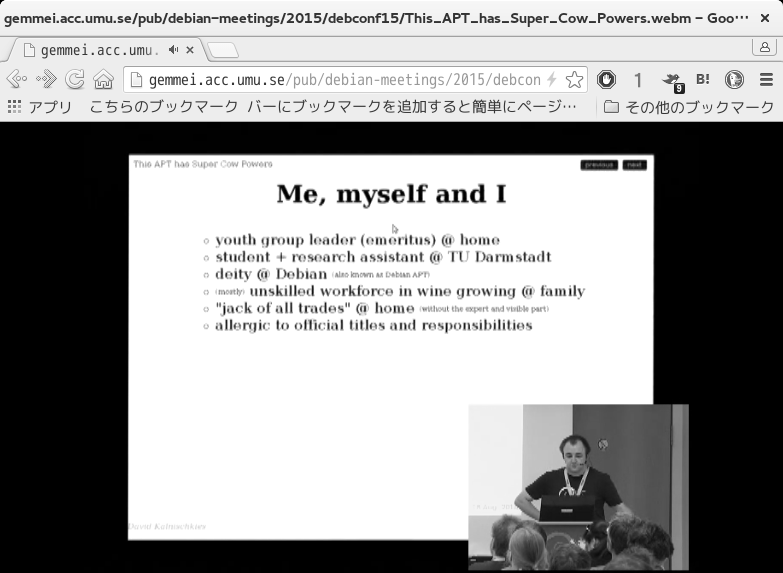
\includegraphics[width=0.5\hsize]{image201508/debconf15-apt_mono.png}
\end{center}
\caption{Debconf15$B$N(BAPT1.1$B$N%;%C%7%g%s$NMM;R(B}
\end{figure}

\subsection{APT 1.1$B$rI>2A$7$F$_$k(B}

$B!!(B2015/8/22$B8=:_!"(BAPT 1.1$B$O(Bexperimental$B%j%]%8%H%j$K$"$j$^$9!#AaB.!";n$7$F8+$?$$J}$O0J2<$N$h$&$K$9$k$3$H$GF3F~$G$-$^$9!#(B

\begin{commandline}
$ sudo vi /etc/apt/source.lists
deb http://ftp.jp.debian.org/debian/ experimental main contrib non-free
deb-src http://ftp.jp.debian.org/debian/ experimental main contrib non-free
$ sudo apt-get update
$ sudo apt-get -t experimental install apt
$ apt
apt 1.1~exp9 (amd64)
Usage: apt [options] command
...$BCfN,(B...
 full-upgrade - upgrade the system by removing/installing/upgrading packages
 edit-sources - edit the source information file
\end{commandline}

 $B<j85$N(BDebian sid$B4D6-$KF3F~$7$F$7$P$i$/;H$C$F$$$^$9$,!"FC$KF0:n$KLdBj$O8+Ev$?$j$^$;$s$G$7$?!#(Bapt update,apt full-upgrade, apt autoremove$B$J$I0lDL$j$NF0:n$OLdBj$J$/$G$-$F$*$j!"CWL?E*$J%P%0$K$bFC$KAx6x$7$F$$$^$;$s!#@'Hs$*;n$7$"$l!#(B

\subsection{APT 1.1$B$NFCD'(B}

$B!!(Bjessie$BEk:\$N(BAPT 1.0.9.8$B$KHf$Y$F$N0c$$$r=R$Y$F$_$^$9!#(B

$B!!@h$K>R2p$7$?(BDebconf15$B$N%S%G%*$K$h$l$P0J2<$NE@$,0c$$$H$J$j$^$9!#(B

\begin{itemize}
\item $B%j%]%8%H%j$N>pJs$N%;%-%e%j%F%#8!>Z$,6/2=$5$l$?!#(B
\item deb822$B7A<0$G%j%]%8%H%j$r;XDj$9$k$d$jJ}$K$F5!G=6/2=!#(B(/etc/apt/*.sources$B%U%!%$%k!K(B
\item httpredir.debian.org$B$r<u$1$F!"=hM}$NESCf7P2a$NI=<($rJQ99!#(B
\item Pinning$B$,$A$c$s$HF0$/$h$&$K$J$C$?!#(B
\item $B0MB84X78$r$9$k>l9g!"%m!<%+%k$K$*$$$?(B.deb$B%U%!%$%k$rD>@\;XDj$7$F$b%$%s%9%H!<%k$G$-!"%=!<%9%S%k%I$N0MB84X78$r;XDj$9$kJ}K!$,=@Fp$K$J$C$?!#(B
\end{itemize}

 $B$^$:$O!"(Bman apt$B!"(Bman apt-get$B$G5-:\$5$l$F$$$kFbMF$G!"%H%T%C%/$r9J$C$F0c$$$r>R2p$7$^$9!#(B

\subsubsection{apt autoremove}

 APT1.1$B$KEk:\$5$l$?(Bapt$B%3%^%s%I$N(Bautoremove$BL?Na$K$D$$$F@bL@$7$^$9!#(B

 $B2?$+%Q%C%1!<%8$r%$%s%9%H!<%k$7$?>l9g!"0MB84X78$rK~$?$9$?$a$@$1$K%$%s%9%H!<%k$5$l$?%Q%C%1!<%8$,2a5n$K$"$k$H$7$^$9!#$3$3$G!"8=:_$O$=$N0MB84X78$+$i$b30$5$l$F$*$j!"$b$O$dA4$/;H$o$l$F$$$J$$%Q%C%1!<%8$,$"$j$^$9!#$3$N%3%^%s%I$r$D$1$F(Bapt$B%3%^%s%I$r5/F0$9$k$H!"$3$&$$$C$?;H$o$l$F$$$J$$%Q%C%1!<%8$r:o=|$9$k$3$H$,=PMh$^$9!#(B

\begin{commandline}
$ sudo apt autoremove
\end{commandline}
%$

\subsubsection{autoremove$B;EAH$_(B}

 autoremove$B$O$I$N$h$&$K$7$F>C5n$9$Y$-%Q%C%1!<%8$r8+$D$1$k$N$G$7$g$&$+!)(B

 $B0MB84X78$,8+Ev$?$i$J$$%Q%C%1!<%8$NCf$K$O!"MxMQ<T$,<+J,$GL@<($7$FF~$l$?%Q%C%1!<%8$b$"$j$^$9!#$=$N$?$a!"I,$:$7$bB>$N%Q%C%1!<%8$G0MB8$7$F$$$J$$$H$$$&$3$H$@$1$r>r7o$K$7$F!"(Bautoremove$B$G%Q%C%1!<%8$r>C$9$h$&$J$3$H$OHr$1$J$1$l$P$J$j$^$;$s!#(Bautoremove$B$K$h$j!"<+F0$G>C5n$7$FNI$$%Q%C%1!<%8$rH=CG$9$k4p=`$O<!$NDL$j$G$9!#(B
 
\begin{description}
 \item [Step 1.] /var/lib/apt/extended\_states$B%U%!%$%k$N5-O?$K!"2a5n!"0MB84X78$rK~$?$9$?$a$K%Q%C%1!<%8$rF3F~$7$?$+$I$&$+$N5-O?$G$"$k(B''Auto-Installed: 1''$B$H5-$5$l$F$$$k%Q%C%1!<%8$r>C5n$N8uJd$H$9$k!#(B
 \item [Step 2.] $B$9$G$K%$%s%9%H!<%k:Q%Q%C%1!<%8$N$I$l$+$i$b0MB84X78$KL5$$$+$I$&$+!)(B
 \item [Step 3.] $B$5$i$K!"(B
\begin{itemize}
\item Recommends$B$H$7$FDs0F$5$l$F$$$k%Q%C%1!<%8$O%$%s%9%H!<%k$7$FM_$7$$$HL@<($7$?>l9g!"(B
\item Suggest$B$H$7$FDs0F$5$l$F$$$k%Q%C%1!<%8$O%$%s%9%H!<%k$7$FM_$7$$$HL@<($7$?>l9g!"(B
\end{itemize}
$B$N$$$:$l$K$b3:Ev$7$F$$$J$$$+!)(B
\end{description}

$B0J>e$N(BStep 1.$B!A(B3.$B$NH=CG$r7P$?%Q%C%1!<%8$,!"<+F0$G>C5n$7$FNI$$%Q%C%1!<%8$H$7$F07$o$l$^$9!#(B

\subsubsection{man apt-get$B$H$N0c$$(B}

$B<!$K(Bman apt-get$B$G8+$?(B1.0.9.8$B$H$N0c$$$K$D$$$F>R2p$7$^$9!#(B

 \begin{itemize}
\item \texttt{indextargets} \\
   apt-get update$B$G99?7$5$l$k%U%!%$%k$H>uBV$r(Bdeb822$B7A<0$GI=<($7$^$9!#(B
 \item \texttt{--allow-downgrades} \\
   $BFCDj%Q%C%1!<%8$r%@%&%s%0%l!<%I$9$k$3$H$K$h$j0MB84X78$,K~$?$;$k$H$-$K!"%f!<%6$K?R$M$:<B9T$7$F$^$&$H$$$&%*%W%7%g%s$G$9!#(B
 \item \texttt{--allow-remove-essential} \\
   $B2?$i$+$NM}M3$K$h$j(BDebian$B%7%9%F%`$NI,?\%Q%C%1!<%8!J(Bessential$B%Q%C%1!<%8$H$7$FJ,N`$5$l$F$$$k!K$b$N$r>C$;$P0MB84X78$,K~$?$;$k$H$-$K!">C$7$F$h$$$+!)$r?R$M$:>C$7$F$7$^$&%*%W%7%g%s$G$9!#(B
 \item \texttt{--allow-change-held-packages} \\
$B!!!!2?$i$+$NM}M3$K$h$j(BHold$B07$$$K$7$?%Q%C%1!<%8$r:o=|$9$l$P0MB84X78$,K~$?$;$k$H$-$K!">C$7$F$h$$$+!)$r?R$M$:>C$7$F$7$^$&%*%W%7%g%s$G$9!#(B
$B!!(B\item \texttt{--no-allow-insecure-repositories} \\
   $B%j%]%8%H%j$K$"$k(BRelease$B%U%!%$%k(B(InRelease$B%U%!%$%k!K$N(BGPG$B$K$h$k=pL>$,3NG'=PMh$J$$Ey!"%;%-%e%j%F%#>eLdBj$,$"$k$H$_$J$5$l$?%j%]%8%H%j$,4^$^$l$?>l9g!"(Bapt-get update$BA`:n$r<:GT$5$;$^$9!#(B
 \end{itemize}
 
 \subsubsection{$B%j%]%8%H%j7xO42=(B}

$B!!(BAPT 1.1$B$O%j%]%8%H%j$N%;%-%e%j%F%#$N@5Ev@-I>2A$,6/2=$5$l$F$$$^$9!#@5Ev@-I>2A$N85$H$J$k%U%!%$%k$K(BRelease$B%U%!%$%k(B(InRelease$B%U%!%$%k!K$,$"$j$^$9!#(B

\begin{commandline}
$ curl http://cloudfront.debian.net/debian/dists/unstable/InRelease
-----BEGIN PGP SIGNED MESSAGE-----
Hash: SHA256

Origin: Debian
Label: Debian
...$BCfN,(B...
MD5Sum:
 e9f9b477f2430a7d0e2dd686da1af507 30975818 Contents-amd64.gz
 d158f809191a841bedf9ff50e34e0ebe 30421142 Contents-armel.gz
...$BCfN,(B...
-----BEGIN PGP SIGNATURE-----
Version: GnuPG v1

iQIcBAEBCAAGBQJV1+IMAAoJEItIrWJGklVTgloP/0+XAch/TMtTSfH+N1QFl+q2
Woas1LpWhHDO12U6vuPq5wghCPYE5ctNuDxFtTy9j01lsf6kWXPDh1QupNENDNHr
lfZ7Qa9gFr8W3tH1tnPwsSqcQmu9bMkR0sRDVSfcFlDioVhN/h+jWW7j7J7nrZrE
...$BCfN,(B...
\end{commandline}
   
InRelease$B%U%!%$%k$r8+$k$H$o$+$k$H$*$j!"(B

\begin{itemize}
\item $B%j%]%8%H%j$K4^$^$l$kMM!9$J%U%!%$%k$OA4$F(Bmd5sum$BIU$-$G(BInRelease$B%U%!%$%k$K5-O?(B
\item $B$5$i$K(BInRelease$B%U%!%$%k$bEE;R=pL>$K$h$k@5Ev@-3NG'$,=PMh$k$h$&$K$J$C$F$$$k(B
\end{itemize}

$B$H$J$j$^$9!#(B

$B!!:#2s(BAPT1.1$B$G$O!"4pK\E*$K(BInRelease$B%U%!%$%k$NL5$$!"$"$k$$$O!"B>$KI,MW$J%U%!%$%k$,7gMn$7$F$$$k$J$I!"%;%-%e%j%F%#4QE@$+$i$N@5Ev@-3NG'$,=PMh$J$$%j%]%8%H%j$O<h$j07$$$r40A4$K$d$a$k@_7W$K$7$?$H$N$3$H$G$9!#(B

\subsubsection{httpredir.debian.org$BBP1~(B}

 2015/5$B7n:"!"(BDebian$B%f!<%6$K:G$b6a$$(Bmirror$B%5!<%P!<$r(BHTTP Redirect$B$G(Bapt$B$K65$($F$/$l$k%5!<%S%9$,2TF/$7$^$7$?!#$D$^$j!"%f!<%6$O(B/etc/apt/sources.list$B$K!"(Bhttpredir.debian.org$B$r;XDj$9$l$P!"%f!<%6$K:G$b6a$$(Bmirror$B%5!<%P!<$X%j%@%$%l%/%H$5$l$^$9!#(B

 $B$3$3$G!"%j%@%$%l%/%H$5$l$?7k2L$I$3$N%5!<%P$+$i<hF@$9$k$N$+!)$,$o$+$k$HJXMx$J;v$,B?$$$G$9!#$3$N$?$a!"(BAPT1.1$B$N(Bapt/apt-get$B$O%j%@%$%l%/%H$5$l$?@h$N>pJs$rI=<($9$k$h$&$KJQ99$5$l$^$7$?!#(B

\subsubsection{$B;29M!'(Bhttpredir.debian.org$B$NMM;R(B}

 httpredir.debian.org$B$,2?$rJV5Q$9$k$N$+$r0J2<$K<($7$^$9!#(B

\begin{commandline}
$curl -v http://httpredir.debian.org/debian/dists/sid/InRelease
> GET /debian/dists/sid/InRelease HTTP/1.1
> Host: httpredir.debian.org
> User-Agent: curl/7.44.0
> Accept: */*
> 
< HTTP/1.1 302 Found
< Date: Sat, 22 Aug 2015 03:54:12 GMT
< Location: http://cloudfront.debian.net/debian/dists/sid/InRelease
< Content-Type: text/plain
...$B>JN,(B...
\end{commandline}    

 $B8+$F$N$H$*$j!"(Bcloudfront.debian.net$B$K%j%@%$%l%/%H$,;X<($5$l$k$N$,3NG'$G$-$k$H;W$$$^$9!#(B

{ \scriptsize
 \begin{itembox}[l]{cloudfront.debian.net?}
 $BA0%Z!<%8$N%j%@%$%l%/%H@h$K$F!"(B
\url{http://cloudfront.debian.net/}
$B$H%j%]%8%H%j$,Ds0F$5$l$F$$$^$9!#$3$l$O!"(B2$BG/A0$K(Bdebian-cloud$B%A!<%`$G%"%J%&%s%9$,$"$C$?!"(BAWS$B$N(Bcloudfront$B$H$$$&(BCDN$B$N;EAH$_$r;H$C$F%G!<%?G[I[$r9T$&;n$_$N%j%]%8%H%j$G$9!#(B
(\url{https://lists.debian.org/debian-cloud/2013/05/msg00066.html})

 $B$b$H$b$H!"(BCDN$B$O%f!<%6$K:G$b8zN(E*$J%5!<%P$rDs<($7$F%G!<%?$rG[$k;EAH$_$G$"$j!"(B
AWS$B$N(Bcloudfront$B$OAjEv$J5,LO$H%5!<%S%9%(%j%"$r;}$D(BCDN$B%5!<%S%9$G$9$N$G!"(B
$B$=$b$=$b$3$A$i$,$"$k$J$i!"(BAWS$B$N%5!<%S%9$,%+%P!<$7$F$$$k9q$G$O!"(Bhttpredir.debian.org$B$r;H$o$J$/$F$9$_$=$&$J5$$b$7$^$9!#$7$+$7$J$,$i!"%=%U%H%&%'%"<+M3$r%b%C%H!<$H$9$k(BDebian$B$H$7$F$O!"0l4k6H$N%5!<%S%9$K0MB8$7$J$$$h$&$K$9$k$3$H$,=EMW$G$9$N$G!"(BDebian$B$H$7$F$O!"(Bhttpredir.debian.org$B$r0];}!&1?MQ$9$kI,MW$,$"$j$^$9!#(B
 \end{itembox}
}

\subsection{deb822$B7A<0(B}

 APT 1.1$B$G$O!"(Bdeb822$B7A<0$G%j%]%8%H%j$r;XDj$9$k$d$jJ}$K$F5!G=6/2=$,?^$i$l$^$7$?!#$3$3$G$O!"(Bdeb822$B7A<0$H$O$I$s$J$b$N$+$r>R2p$7$^$9!#(B

 APT1.1$B$,<j85$K$"$l$P!"4JC1$K(Bdeb822$B7A<0$G%j%]%8%H%j$N>pJs$rI=<($5$;$k;v$,=PMh$^$9!#(B

\begin{commandline}  
$ apt-get indextargets
MetaKey: main/source/Sources
ShortDesc: Sources
Description: http://ftp.jp.debian.org/debian sid/main Sources
URI: http://ftp.jp.debian.org/debian/dists/sid/main/source/Sources
Filename: /var/lib/apt/lists/ftp.jp.debian.org_debian_dists_sid_main_source_Sources
Optional: no
Codename: sid
...$BCfN,(B...
\end{commandline}  
  
 $B=PNO$5$l$k%U%)!<%^%C%H$r8+$k$H$o$+$k$N$G$9$,!"(BRFC822$B%X%C%@$N7A<0$K$h$/;w$F$$$^$9!#$3$3$+$i!"(Bdeb822$B$HL>A0$r<h$C$?$h$&$G$9!#(B

  $BFCD'$H$7$F!"(BRFC822$B$HF1MM$G$9$N$G!"%X%C%@$rA}$d$;$P!"4JC1$K5!G=3HD%$G$-$k$H$$$&E@$,>e$2$i$l$^$9!#(B

  $B$^$?!"F0:nL$3NG'$G$9$,!"(BDebConf15$B$N%S%G%*$K$h$l$P!"(B
\begin{quote}
  /etc/apt/source.list.d/xxxx.sources
\end{quote}
$B!JKvHx$,!"(B.sources$B$G$"$k;v$,I,MW!K$H$$$&L>A0$G(Bdeb822$B7A<0$GCV$$$F$*$/$H!"(B
$B$3$A$i$r(Bsources.list$B$K;XDj$7$?$N$HF1MM$NF0:n$r(Bapt/apt-get$B$O9T$&$H$N$3$H$G$9!#(B
  
\subsection{$B5m$5$s%Q%o!<7r:_(B!}

 APT 1.1$B$K$b(B ``moo'' $BL?Na$O7r:_$G$9!#B)H4$-$K!"$3$A$i$r>R2p$7$F$*$-$^$9!#(B

 man apt$B$K$O5-:\$NL5$$%*%W%7%g%s$G$9$,!"0J2<$K(Bapt$B$N>l9g$N5/F0J}K!$r:\$;$^$9!#(B

\begin{commandline}  
$ apt moo 
$ apt moo moo [--color]
$ apt moo moo moo  
$ faketime '1997-04-01' apt moo
\end{commandline}    

\begin{figure}[H]
\begin{center}
 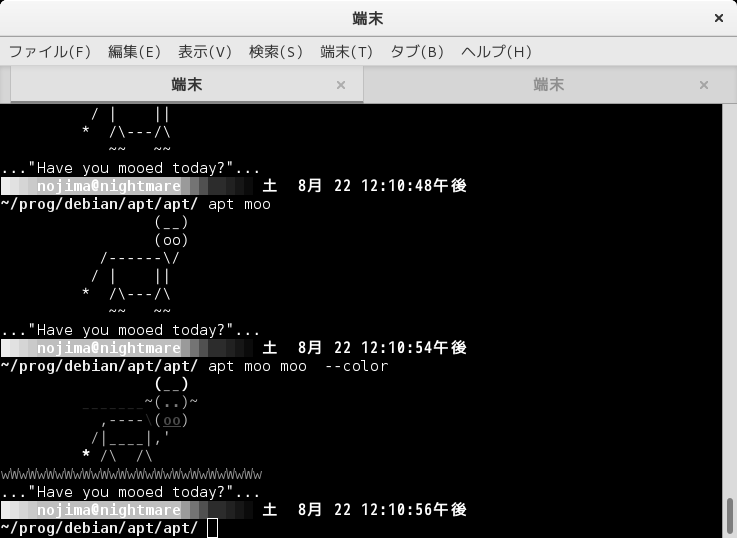
\includegraphics[width=0.7\hsize]{image201508/apt-moo_mono.png}
\end{center}
\caption{apt moo$B%3%^%s%I7k2LNc(B}
\end{figure}

 $B<B9T$9$k$H$o$+$k$N$G$9$,!"(BASCII$B%-%c%i%/%?$GIA2h$5$l$?3F<o$N5m$N3($,I=<($5$l$^$9!#(B

\subsection{$B$*$o$j$K(B}

 $B$^$@$^$@!"(BAPT1.1$B$K$D$$$F!":#2s$3$3$G$O=q$-$-$l$J$$Dx$NJQ99$,2C$($i$l$F$$$k$h$&$G$9$,!"$3$N$X$s$K$7$F$*$-$^$9!#<B:]!"(Bgit$B$GMn$H$7$F:9J,$r3NG'$7$^$7$?$,!"<B$K(B2$BK|9T$rD6$($kJQ99$,9T$o$l$F$$$^$7$?!#@5<0%j%j!<%9$K$J$C$F!"%I%-%e%a%s%H$b=<<B$9$k$HNI$$$G$9$M!#(B
   
%201507tokyo
%-------------------------------------------------------------------------------
\dancersection{Debian$B$G(BHTTP/2$B$r;n$9(B}{$BLnEg(B $B5.1Q(B}
%-------------------------------------------------------------------------------

\subsection{$B$O$8$a$K(B}

 2015/5$B$K(BHTTP/2$B$,(BRFC7540$B$H$7$F?k$KJ8>O2=$5$l$^$7$?!#$^$?!":G6a$G$b!"$[$&$\$&$G(BWEB$B%Z!<%8$"$k$$$O%5!<%S%9$K$D$$$F!"(BHTTP/2$B$NBP1~EY9g$$$K$D$$$FJ9$+$l$k$h$&$K$J$C$F$-$^$7$?(B\footnote{$BK?M-L>7HBSEEOC%$%Y%s%H$G(BHTTP/2$B$r%"%W%j3+H/<T$KA4NO?d>)$7$F$$$k7o$r8+$F%^%B92$F$?$j$7$?$N$OHkL)(B...}$B!#(B

 $B$3$3$G$O!"(BDebian$B$G!"(BHTTP/2$B$N4D6-$r$A$g$C$H:n$C$F;n$7$F$_$^$7$?!#(B

\subsection{$B$H$3$m$G(BHTTP/2$B$C$F!)(B}

  WEB$B%V%i%&%6$,%5!<%P$HDL?.$9$k:]$K!"(BHTTP/1.x(x$B$O(B0,1$B$N?t;z!K$,D9G/(B(HTTP/1.1$B$O(B15$BG/0J>e$b!*(B)$B;H$o$l$F$$$^$9!#$7$+$7$J$,$i!":r:#$N(BWEB$B%Z!<%8$O!"(BHTTP/1.x$B$,:vDj$5$l$?:"$KHf$Y$F3JCJ$K%j%C%A$J%Z!<%8$H$J$C$F$*$j!"#1%Z!<%8$rI=<($9$k0Y$KI,MW$JDL?.NL$O3JCJ$KA}$($F$$$^$9!#(BHTTP/1.x$B$N$^$^$G$O!"(BWEB$B$NDL?.$,Hs8zN($H$J$C$F$7$^$$$^$7$?!#(B

 HTTP/1.1$B$N7gE@$r9nI~$9$k$?$a$K!"(Bgoogle$B<R$G(BSPDY$B$,3+H/$5$l!"$5$i$K(BSPDY$B$r;29M$K$7$F!"Bt;3$N?M$N9W8%$K$h$j!"<!@$Be$N(BHTTP$BDL?.5,3J$,:vDj$5$l$^$7$?!#$3$l$,(BHTTP/2$B$H$J$j$^$9!#(B

 \subsection{HTTP/2$B$NFCD'(B}

 HTTP/2$B$NFCD'$H$7$F$O0J2<$NDL$j$G$9(B\cite{ref:http-2-faq}$B!#(B
 
\begin{itemize}
\item $B%F%-%9%HEEJ8%Y!<%9$G$O$J$/!"%P%$%J%jEEJ8$r;H$$$^$9!#(B
\item $B#1K\$N(BTCP$B%3%M%/%7%g%s>e$G!"J#?t$N%j%/%(%9%H!&%l%9%]%s%9$rB?=E2=$7$F$d$j$H$j$G$-$k$h$&$K@_7W$5$l$F$$$^$9!#(B
\item  $B%j%/%(%9%H!&%l%9%]%s%9$K;H$o$l$k%X%C%@>pJs$rL5BL$NL5$$EEJ8$K$7!"$5$i$K05=L$7!"$h$j8zN(E*$KDL?.$G$-$k$h$&$K$7$F$$$^$9!#<B$O%b%P%$%kC<Kv$J$I$G$O!"%Q%1%C%H$N1}I|$K$+$+$k;~4V$,D9$$$N$G!"%j%/%(%9%H!&%l%9%]%s%9$N3+;O#1%Q%1%C%HL\$K$G$-$k$@$1>pJs$r5M$a9~$`$3$H$ODL?.;~4V$r=L$a$k$N$KHs>o$KM-8z$G$9!#(B
\item $B#1$D$N%j%/%(%9%H$G!"%V%i%&%6$,B3$1$FI,MW$H$9$k%G!<%?$r$^$H$a$F%l%9%]%s%9$G$-$k5!G=$,F~$j$^$7$?!J%5!<%P%W%C%7%e$H$$$&5!G=!#(B)\cite{ref:server-push-primer}
 \end{itemize}

\subsection{HTTP/2$B$5$i$K>\$7$/(B}

  $B$3$l0J>e(BHTTP/2$B%W%m%H%3%k$K$D$$$F!">\$7$/D4$Y$?$$?M$O!"(B

 \begin{itemize}
  \item HTTP/2$BK\2H(B\\
    \url{https://http2.github.io/}
  \item $B9bB.!&Bg5,LO%M%C%H%o!<%/;~Be$K8~$1$F2~NI$5$l$?(BHTTP/2$B%W%m%H%3%k(B
    \url{http://www.atmarkit.co.jp/ait/articles/1409/18/news135.html}
  \item twitter$B$N(B\#http2study$B%?%0(B
  \item http/2 Advent Calender 2014
    \url{http://qiita.com/advent-calendar/2014/http2}
\end{itemize}

 $B$J$I$J$I!"B??t$NNI$$2r@b$,$"$j$^$9$N$G@'Hs$4Mw$/$@$5$$!#$3$l0J>e:Y$+$$(BHTTP/2$B$N%W%m%H%3%k;EMM$K$D$$$F$O$3$3$G$O3d0&$7$^$9!#(B

 \subsection{HTTP/2$B$NNI$$%G%b%5%$%H(B}

 $BO@$h$j>Z5r$G!"(BHTTP/2$B$,M%$l$F$$$k$+!)$r;n$;$kHs>o$KNI$$%G%b%5%$%H$,$"$j$^$9!#@'Hs$*;n$72<$5$$!#$J$*!"(BDebian sid$B$N(Bchromium/iceweasel$B$GF0:n3NG'$r3NG'$G$-$F$$$^$9!#(B
 \\
\begin{center} 
 \url{https://http2.golang.org/gophertiles}
\end{center}

\subsection{HTTP/2$B$NDL?.3+;O$N;EJ}(B}

 HTTP/2$B$r;H$C$F%V%i%&%6$+$i%"%/%;%9$9$k$H$-!"8=>u!"(BTLS$B$N(BALPN/NPN$B$G(BHTTP/2$B$r;XDj$7$F!"$d$j$H$j$r3+;O$9$k$d$jJ}$7$+8=9T%V%i%&%6$K$O<BAu$5$l$F$$$^$;$s!#$H$$$&$o$1$G!";v<B>e!"(BHTTP/2$B$N%5%$%H$O!"A4It%U%k(BSSL$B2=$5$l$F$$$k>u67$H$J$j$^$9(B\cite{ref:wikipedia-http-2}$B!#(B

 $B0lJ}!"(BTLS$B$r;H$o$J$$>l9g!"(BHTTP/1.1$B$N%j%/%(%9%H%X%C%@$KFCJL$J%X%C%@$r:.$<$k$3$H$K$h$j!"(BHTTP/2$B$X%"%C%W%0%l!<%I$7$F!"0J9_(BHTTP/2$B$G$d$j<h$j$r$9$k$H$$$&<jK!$,$"$j$^$9!#$7$+$7$J$,$i!"$3$A$i$O%V%i%&%6$,BP1~$7$F$$$^$;$s(B\cite{ref:http-2-protocol-upgrade-primer}$B!#(B

\subsection{Debian$B$G(BHTTP/2$B$r$*<j7Z$K3Z$7$`(B}

 HTTP/2$B$r(BDebian$B$G$*<j7Z$K3Z$7$`$K$O0J2<$N4D6-$rMQ0U$7$^$9!#(B

 \begin{itemize}
  \item $B%/%i%$%"%s%HB&=`Hw(B\\
    chromium$B$+!"(Biceweasel
  \item $B%5!<%P!<B&=`Hw(B\\
     nghttp2,Apache Traffic Server$BEy$J$I(B
 \end{itemize}  
 
 \subsection{$B%/%i%$%"%s%HB&=`Hw(B}

 $B0J2<$K(Bchromium$B$H!"(Biceweasel$B$K$D$$$F!"(BHTTP/2$BMQ$rI>2A$9$k$N$KJXMx$J%;%C%H%"%C%W$K$D$$$F:\$;$^$9!#(B

 \subsubsection{chromium}

 chromium$B$r;H$&>l9g$O<!$NDL$j$G$9!#$^$:!"(BDebian$B$K(Bchromium$B%V%i%&%6$rF3F~$7$^$9!#(B
  
\begin{commandline}
$ sudo apt-get install chromium
\end{commandline}
% $
$B<!$K!"(Bchromium$B$r5/F0$7$F:86y$_$K8=$l$k!V(BApps$B!W(B$\rightarrow$$B!V(BWeb Store$B!W$r%"%/%;%9$7!"!V(BHTTP/2 and SPDY indicator$B!W$rF3F~$7$F$/$@$5$$!#(B

$B!!0J>e$NA`:n$r9T$C$?(Bchromium$B$G(BHTTP/2$BBP1~$N%5%$%H$K%"%/%;%9$9$k$H!"@D$$0p:J%^!<%/$,%"%I%l%9%P!<$KI=<($5$l$k$h$&$K$J$j$^$9!#(B

\begin{figure}[H]
\begin{center}
 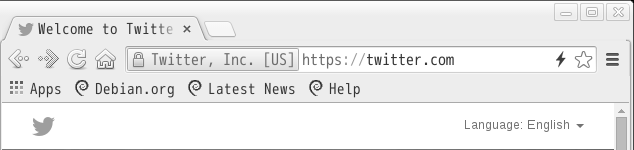
\includegraphics[width=0.9\hsize]{image201507/chromium-http-2-ready_mono.png}
\end{center}
\caption{chromium$B$G(BHTTP/2$B$N%5%$%H$K%"%/%;%9(B}
\end{figure}

\subsubsection{iceweasel}

 iceweasel$B$r;H$&>l9g$O<!$NDL$j$G$9!#$^$:!"(Biceweasel$B$H!"(Bxul-ext-spdy-indicator$B$r(BDebian$B$KF3F~$7$^$9!#(B
  
\begin{commandline}
$ sudo apt-get install iceweasel xul-ext-spdy-indicator
\end{commandline}
% $

$B0J>e$NA`:n$r9T$C$?(Biceweasel$B$G(BHTTP/2$BBP1~$N%5%$%H$K%"%/%;%9$9$k$H!"@D$$0p:J%^!<%/$,%"%I%l%9%P!<$KI=<($5$l$k$h$&$K$J$j$^$9!#(B

\begin{figure}[H]
\begin{center}
 
\includegraphics[width=0.9\hsize]{image201507/iceweasel-http-2-ready_mono.png}
\end{center}
\caption{iceweasel$B$G(BHTTP/2$B$N%5%$%H$K%"%/%;%9(B}
\end{figure}

\subsection{$B%5!<%PB&=`Hw(B}

$B!!$$$h$$$h(BDebian$B$K%5!<%PB&$r=`Hw$7$^$9!#(B

\subsubsection{HTTP/2$B$KBP1~$7$F$$$k%5!<%P(B}

 $B$I$s$J%5!<%P$,(BHTTP/2$B$KBP1~$7$F$$$k$+$O!"(B\\
\\
 Implementations \\
  \url{https://github.com/http2/http2-spec/wiki/Implementations}\\
\\
 $B$r;2>H$/$@$5$$!#(B

\subsubsection{nghttp2$B%Q%C%1!<%8(B}

 Debian sid$B$K$F!"(BHTTP/2$BBP1~%5!<%P$N%Q%C%1!<%8$H$7$F!"(Bnghttp2$B$,$"$j$^$9!#$3$3$G$O$3$A$i$r;H$C$F%5!<%P$r:n$k$3$H$K$7$^$9!#(B

 \begin{commandline}
$ sudo apt-get install nghttp2 ssl-cert
\end{commandline}
% $

 $B$J$*!"1\Mw2DG=$J%3%s%F%s%D$H$7$F!"(Bgroff$B$NIUB0(Bhtml$B%^%K%e%"%k$r%I%-%e%a%s%H%k!<%H$K$7$?(BHTTP/2$B%5!<%P$rN)$F$F$_$^$9!#(B

  $B$J$*!"(B*-snakeoil.*$B$H$$$&%U%!%$%k$O!"(Bssl-crt$B%Q%C%1!<%8$rF3F~$9$k$H>!<j$K:n@.$5$l$k<+8J>ZL@=q%U%!%$%k$H$J$j$^$9!#(B
  
\begin{commandline}
$ sudo nghttpd -D -d /usr/share/doc/groff-base/html/ \
  443 /etc/ssl/private/ssl-cert-snakeoil.key \
  /etc/ssl/certs/ssl-cert-snakeoil.pem
\end{commandline}  
%$

\subsection{$B%"%/%;%9$7$F$_$k(B}

  $B%V%i%&%6$G!"%"%/%;%9$7$F$_$^$9!#(B\\
 $B%"%/%;%9@h!'(B\url{https://localhost/pic-6.html}

 chromium/iceweasel$B6&$KL5;v$K(BHTTP/2$BBP1~$r<($9@D$$0p:J%^!<%/$,(BURL$BI=<(ItJ,$KIU$$$F$$$k$3$H$,H=$j$^$9!#(B

\begin{minipage}{0.5\hsize}
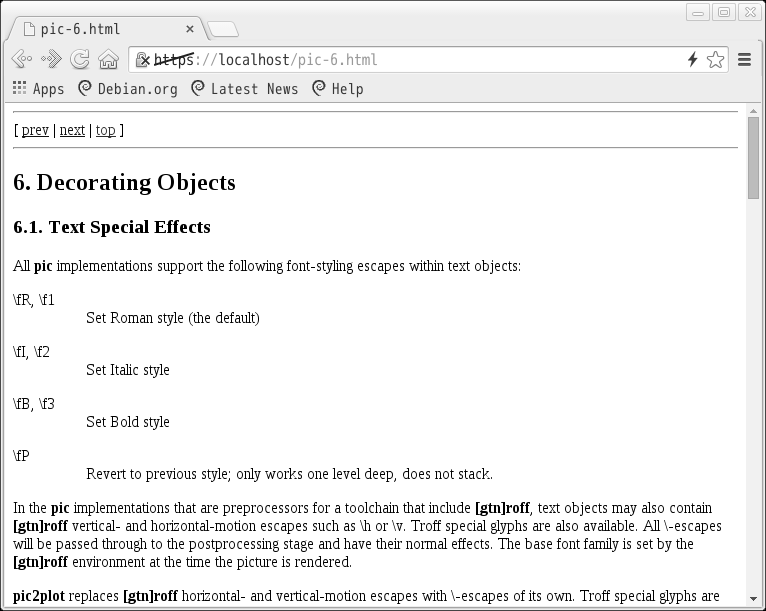
\includegraphics[width=0.9\hsize]{image201507/chromium-groff-access_mono.png}
\end{minipage}
\begin{minipage}{0.5\hsize}
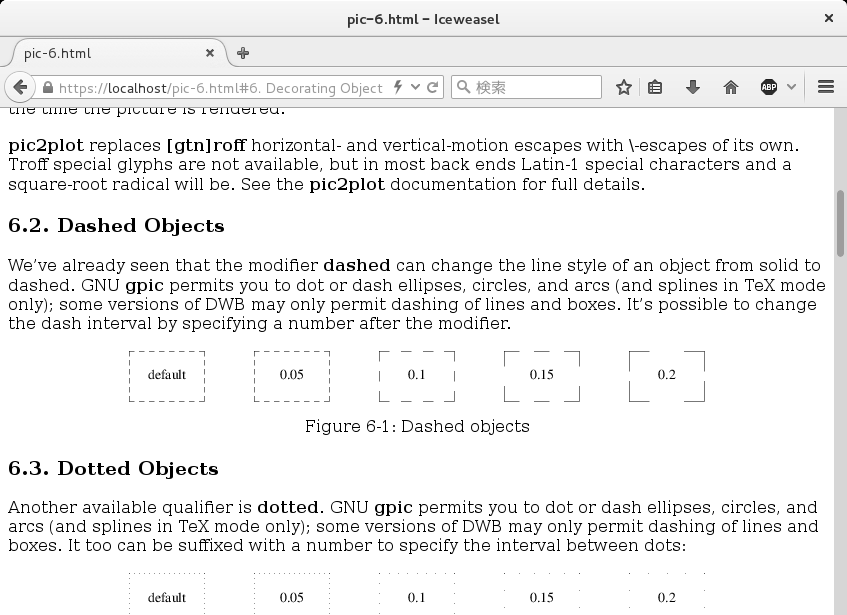
\includegraphics[width=0.9\hsize]{image201507/iceweasel-groff-access_mono.png}
\end{minipage}
 
\subsection{proxy$B%5!<%P$G4{B8%5%$%H$N(BHTTP/2$B2=$r$d$C$F$_$k(B}

$B!!$5$F!"(Bnghttpd$B$O7ZNL$N(BHTTP/2$BBP1~(BWEB$B%5!<%P$G$O$"$k$N$G$9$,!"$d$C$Q$j(Bapache$B$N$h$&$J9b5!G=$J(BWEB$B%5!<%P$r;H$C$F(BHTTP/2$B$r<B8=$7$?$$$H$$$&%K!<%:$,$"$k$H;W$$$^$9!#!JNc!'(Bphp$B$N%5%$%H$r(BHTTP/2$B2=$7$?$$Ey!K(B

 $B:#EY$O!"(Bapache$B$r%P%C%/%(%s%I$K$7$F!"(Bnghttp2$BIUB0$N(Bproxy$B%5!<%P$r;H$$!"%5%$%H$N(BHTTP/2$B2=$r9T$C$F$_$^$9!#(B
  
 $B:#2sMQ0U$7$h$&$H$7$F$$$k4D6-$N35G0?^$r:\$;$^$9!#(B

\begin{figure}[H]
\begin{center}
 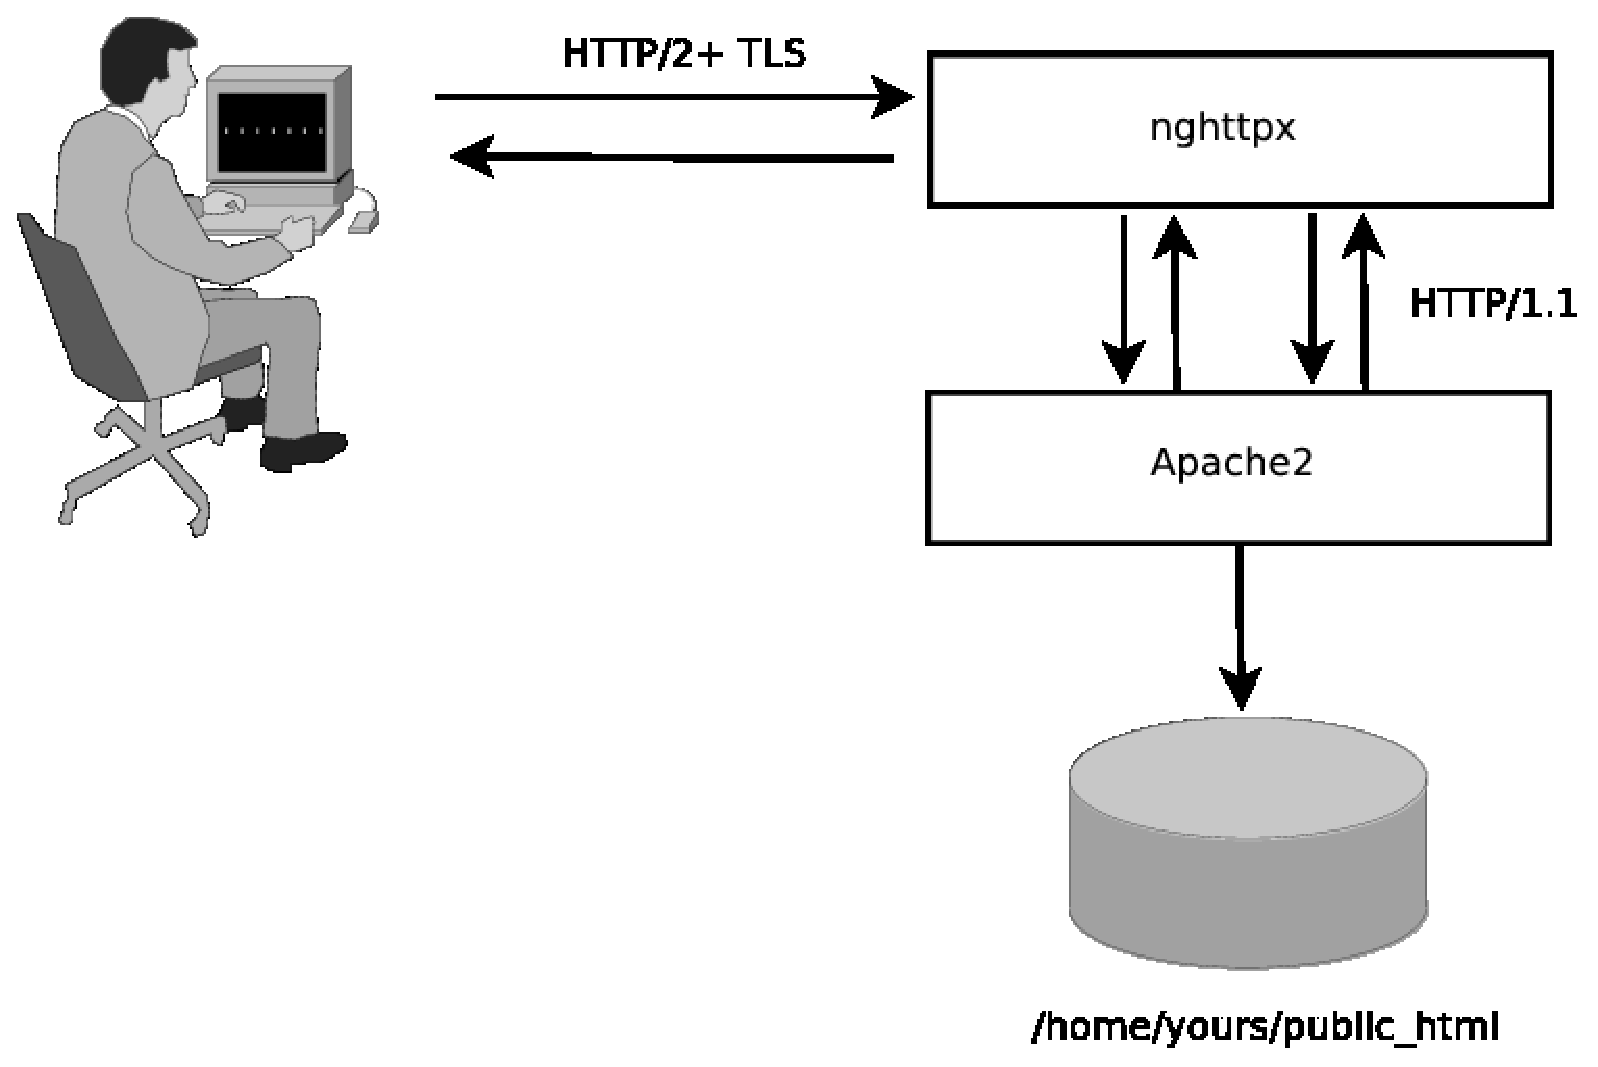
\includegraphics[width=0.5\hsize]{image201507/nghttpx-apache-proxying-mono.eps}
\end{center}
\caption{proxy$B%5!<%P$G(BHTTP/2$B2=$r9T$&4D6-$N35G0?^(B}
\end{figure}
  
 proxy$B$H(Bapache$B$N4D6-$r(BDebian$B$KMQ0U$7$^$9!#<j=g$O<!$NDL$j$G$9!#(B

\begin{description}
\item [Step 1.] sudo apt-get install apache2 nghttp2 ssl-cert
\item [Step 2.] sudo a2enmod userdir
\item [Step 3.] cd /home/yours/; mkdir public\_html
\item [Step 4.] cd public\_html; cp -a /usr/share/doc/groff-base/html .
\item [Step 5.] sudo vi /etc/nghttpx/nghttpx.conf\\
\begin{commandline}
 ----nghttpx.conf$B$NCf?H$3$3$+$i(B----
frontend=0.0.0.0,443 
backend=127.0.0.1,80 
private-key-file=/etc/ssl/private/ssl-cert-snakeoil.key 
certificate-file=/etc/ssl/certs/ssl-cert-snakeoil.pem 
workers=1 
----$B$3$3$^$G(B----
\end{commandline}
\item [Step 6.] sudo systemctl start apache2.service
\item [Step 7.] sudo nghttpx -D --conf /etc/nghttpx/nghttpx.conf
\end{description}

$B!!0J>e$G$-$^$7$?$i!"$$$h$$$h@h$KMQ0U$7$?%V%i%&%6$+$i%"%/%;%9$7$F$_$^$9!#L5;v(B apache$BB&$KMQ0U$7$?%5%$%H$,!"(BHTTP/2$BBP1~$G$-$F$$$k;v$,$o$+$j$^$9!#(B\\
\\
$B!!%"%/%;%9@h!'(B\url{http://localhost/~yours/html/pic.html}\\

\subsection{$B$*$o$j$K(B}

  HTTP/2$B$b(BDebian$B$r;H$($P4JC1$K<B83$G$-$^$9!#$^$?!"Bt;3$N%U%!%$%k$G9=@.$5$l$k%Z!<%8$,$"$k$H!"(BHTTP/2$B$OHs>o$K0RNO$rH/4x$7$^$9!#$3$N5!2q$K(BHTTP/2$B$r@'Hs$*;n$7D:$-!"$=$N0RNO$r3NG'$7$F$_$F$/$@$5$$!#(B
  
\begin{thebibliography}{9}
\bibitem{ref:http-2-faq} HTTP/2 Frequently Asked Questions,\url{https://http2.github.io/faq/}
\bibitem{ref:server-push-primer} $B=i$a$F$N(BHTTP/2$B%5!<%P%W%C%7%e(B,\url{http://labs.gree.jp/blog/2014/12/11987/}
\bibitem{ref:wikipedia-http-2} wikipedia HTTP/2$B$N>O(B,\url{https://ja.wikipedia.org/wiki/HTTP/2}
\bibitem{ref:http-2-protocol-upgrade-primer} HTTP/2 $B%W%m%H%3%k%M%4%7%(!<%7%g%sJ}K!$H(B ATS $B$G$N<BAu(B,\url{http://techblog.yahoo.co.jp/infrastructure/http2/ats_http2_pn/}
\end{thebibliography}

%201510 tokyo
%-------------------------------------------------------------------------------
\dancersection{NTT $B%U%l%C%DLV7PM3$G(BNative IPv6}{Roger Shimizu}
%-------------------------------------------------------------------------------
\subsection{$B$O$8$a$K(B}
NTT $B%U%l%C%D$r;H$C$F$$$k<+Bp$G(BIPv6$B%$%s%?!<%M%C%H$,F0$+$J$+$C$?$s$G$9!#(B
\\
NTT NGN $BLV$r;H$&$H!"$I$3$+$+$i(BIPv6 $B%"%I%l%9$,3d$jEv$F$i$l$^$9$7!"%2!<%H%&%'%$$b<+F0E*$K@_Dj$5$l$^$9$,!"(BInternet$B$K7R$,$i$J$$!*(B
\\
$B860x$O!"(BDual $B%9%?%C%/BP1~:Q$_(BDNS $B$,(B AAAA record (IPv6 address) $B$N7k2L$r!"(BA record $B$H0l=o$KJV$7$^$9!#(B
\begin{itemize}
\item Google$B!G(Bs DNS: 8.8.8.8 / 8.8.4.4
\item NTT$B!G(Bs DNS: 129.250.35.250 ($B4XEl(B) / 129.250.35.251 ($B4X@>(B)
\end{itemize}
OS$BB&$G$O!"(BIPv6 $B$,$"$l$P!"(BIPv4 $B$h$j(BIPv6 $B$,M%@hE*$K;H$o$l$^$9!#(B
\\
$B$7$+$7!"(BIPv4$B$X$N%U%)!<%k%P%C%/$,H/@8$7$F%M%C%H%"%/%;%9$,Hs>o$KCY$/$J$C$F$7$^$&!#(B
\\
NTT $B$G$O$=$&$$$&>u67$,GD0.$5$l$F$$$k$h$&$G$9!"$=$N2r7hJ}K!$O$J$s$H!V(BIPv6 $B$rL58z!W(B\footnote{\url{https://flets.com/customer/ipv6_display.html}}$B$H$J$j$^$9!*(B
\\
\subsection{Debian$B$G$O$I$&$d$C$F(BIPv6 $BL58z$9$k$N!)(B}
kmod $B@_Dj%U%!%$%k(B(squeeze$B$^$G;HMQ2DG=(B): /etc/modprobe.d/aliases
\begin{commandline}
alias net-pf-10 off
\end{commandline}
sysctl $B@_Dj%U%!%$%k(B($BF0E*$KJQ992DG=(B): /etc/sysctl.conf
\begin{commandline}
net/ipv6/conf/all/disable_ipv6 = 1
\end{commandline}
$B5/F0;~$N(B kernel $B%Q%i%a!<%?(B($B:G=i$+$iL58z$K$J$k(B): 
\begin{commandline}
ipv6.disable=1
\end{commandline}
/etc/default/grub $B$N(B GRUB\_CMDLINE\_LINUX $BJQ?t$KDI2C$,I,MW$G$9!#(B
Debian Installer $B$J$i!"5/F0;~$K(B\verb|<TAB>| $B$r$7$F$+$i>e5-$N%Q%i%a!<%?$rF~NO$G$-$^$9!#(B
\\
\subsection{IPv6 $BBN83$N$?$a$N(B $B%H%s%M%kJ}<0$N;H$$J}(B}
Native $B4D6-$,8+$D$+$i$J$1$l$P!"%H%s%M%kJ}<0$G$J$I?'!9BN83$9$kJ}K!$,$"$j$^$9!#(B
\begin{itemize}
		\item 6in4 (proto-41) ($BNc$(!"(B{\tt Hurricane Electric $B$5$s$N(B tunnelbroker $B%5!<%S%9(B}\footnote{\url{https://www.tunnelbroker.com}})
\item Teredo ($BNc$(!"(BDebian $B$G(B miredo $B$H$$$&%Q%C%1!<%8$r%$%s%9%H!<%k$9$l$P$9$0$K;H$($^$9(B)
\item SixXS
\item AICCU
\item AYIYA
\item 6to4 (via 192.88.99.1)
\item 6over4 (fe80:: \& IPv4)
\item freenet6
\end{itemize}
$BBN83!&8!>Z$0$i$$$J$i$=$l$GNI$$$1$I!"=>Mh(B IPv4 $B$N@-G=$HHf$Y$FCY$/$F!"DL>o$K(B IP $B%H%s%M%k$r;HMQ$9$k$3$H$O$*$9$9$a$7$J$$$H9M$($F$*$j$^$9!#(B
\subsection{Tunnel $B$GCY$/$J$k860x$N2r@O(B}
$BIaDL$K%&%'%V%"%/%;%9$,(B Tunnel $B7PM3$J$iCY$/$J$k860x$O(B DNS + CDN $B$H$J$j$^$9!'(B
\begin{itemize}
\item DNS $B$N%l%9%]%s%9;~4V(B
\item CDN $B$N%"%/%;%9;~4V(B
\end{itemize}
DNS $B$O$I$3$r;H$&$Y$-!)Nc$H$7$F!"%"%a%j%+@>3$4_$N(B tunnelbroker.net $B$r;H$&$J$i!"%1!<%9JL$G2r@O$7$F8+$^$7$g$&!#(B
\begin{itemize}
\item Local DNS
\\$B%W%m%P%$%@!<(B(ISP) $B$+$iDs6!$5$l$k(B DNS $B$H$J$j!"(BIPv4 $B$G(B CDN $B$,F|K\$N%5!<%P$KD>@\%"%/%;%9=PMh$F!"FC$KLdBj$,$J$$$1$l$I!"(B
IPv6 $B$@$H(B Host $\rightarrow$ US Tunnel $\rightarrow$ JP CDN $B$K$7$F$7$^$$!"1}I|$G(B 250ms $B0L$K$J$j$^$9!#(B
\item Remote DNS
\\$B%H%s%M%k7PM3$G(B US $BB&$N(B DNS $B$H$J$j!"Kh2s(B DNS query $B$N%3%9%H$,(B 120ms $B0L$K$J$j$^$9$7!"(BIPv4/IPv6 $BN>J}%&%'%V%"%/%;%9;~4V$b(B 120ms $B$r2C;;$5$l$k$H$J$C$F$7$^$$$^$9!#(B
\end{itemize}
$B$I$C$AB&$N(B DNS $B$r;H$C$F$b!"CY$/$J$k$3$H$,J,$+$j$^$7$?!#(B
\subsection{NTT $B%U%l%C%D$G(B Native IPv6 $B$,$G$-$^$9!*(B}
Native IPv6 $B$N%a%j%C%H$H$$$&$H!"(BLocal DNS $B$r;H$&$3$H$G!"(BDNS Query $B%3%9%H$,$"$^$j3]$+$i$J$$$7!"(BIPv4/IPv6 $BN>J}6&$K%m!<%+%k(B($BKt$O6a$/$K(B) CDN $B$,;H$($^$9!#(B
$BB?$/%W%m%P%$%@!<$O(B IPv6 $B$,BP1~$9$k$h$&$K$J$j$^$7$?!#(B
\begin{itemize}
\item OCN: \url{http://service.ocn.ne.jp/ipv6/access/}
\item Plala: \url{http://www.plala.or.jp/ipv6/service/area/}
\item So-net: \url{http://www.so-net.ne.jp/common/IPv6/}
\item $BB>$N(BISP: \url{http://www.jaipa.or.jp/ipv6/}
\end{itemize}
$B$9$Y$F$O3NG'$7$F$$$^$;$s$,!"<g$J(B OCN/So-net/Plala $B$J$I$O4{$K(B Native IPv6 $B$,BP1~$5$l$F$$$k$h$&$G$9!#$=$l$+$i!"4JC1$K(B Dual Stack $B$,9=C[=PMh$^$9!*(B
\subsection{$B6qBNE*$J(B IPv6 $B$N@_DjJ}K!(B}
Dual Stack $B$J$i!"#2K\(BPPP$B%;%C%7%g%s$,I,MW!#Nc$($P!"(B
\begin{itemize}
\item ppp0: IPv4
\item ppp1: IPv6
\end{itemize}
IPv4 $B$N(B PPPoE $B@_Dj$O=>MhDL$j$GNI$/$F!"(BIPv6 $B$NJ}$O(B IPv4 $B$N@_Dj$r%Y!<%9$K$7$F!"0J2<$NJQ99$,I,MW$H$J$j$^$9!#(B
\begin{itemize}
\item cp /etc/ppp/peers/dsl /etc/ppp/peers/dslv6
\item echo +ipv6 \verb|>>| /etc/ppp/peers/dslv6
\item /etc/ppp/peers/dslv6 $B$K!"85(BIPv4$B$N%"%+%&%s%H$r(BIPv6 $BHG$K=q49$($k(B
\item /etc/ppp/chap-secrets $B$K!"(BIPv6 $B%"%+%&%s%H$N%Q%9%o!<%I$rDI2C$7$^$9(B(ID$B$O(B IPv4 / IPv6 $BJL$J$1$I!"%Q%9%o!<%I$O0l=o$K$J$k%1!<%9$,$[$H$s$I$G$9(B)
\end{itemize}
IPv6 PPPoE $B%"%+%&%s%H(B(CHAP ID)$B$K$D$$$F$O!"%W%m%P%$%@!<$K$h$j$^$9!#(B
\\$BNc$H$7$F$O!"(B($BB@;z$O(B IPv4 $B$N@_Dj$K2C$($?ItJ,$G$9(B)
\begin{itemize}
\item {\tt OCN:}\footnote{\url{http://service.ocn.ne.jp/ipv6/access/flow/}}blah@\texttt{ipv6.}ocn.ne.jp
\item {\tt OCN biz:}\footnote{\url{http://www.ocn.ne.jp/business/ftth/withf/spec.html}}blah@bizf\texttt{6}.ocn.ne.jp $BKt$O(B blah@bizd\texttt{6}.ocn.ne.jp
\item {\tt Plala:}\footnote{\url{http://www.plala.or.jp/ipv6/access/flow/}}blah@\texttt{v6h.}plala.or.jp $BKt$O(B blah@\texttt{v6m.}plala.or.jp
\item {\tt So-net:}\footnote{\url{http://www.so-net.ne.jp/option/others/ipv6/}}taro@aa2\texttt{-v6}.so-net.ne.jp
\end{itemize}
$B$^$?!"(BIPv6 address $B$H(B default route $B$b$=$l$>$l@_Dj$,I,MW$G$9!#(B
\begin{itemize}
\item IPv6 address $B$O(B DHCPv6 $B%/%i%$%"%s%H(B (wide-dhcpv6-client$B$J$I(B) $B$G<hF@$7$^$9!#(B
\item IPv6 default route $B$O<jF0@_Dj$H$J$j!"(B\footnote{\url{https://bugs.debian.org/477245}}\footnote{\url{https://github.com/paulusmack/ppp/issues/40}}
\begin{commandline}
ip -6 r add default dev ppp1
\end{commandline}
$B$G:Q$_$^$9!#(B
\end{itemize}
$B@_Dj$N;29M(B: \url{https://youtu.be/bJ9p2j9frtA}
(git repo: \url{https://github.com/rogers0/config/tree/network/flets-native-v4v6})
\subsection{$BMQ8lDj5A(B}
\begin{itemize}
\item stateless host: IPv6 address $B$H(B default gateway $B$O(B RA ($B%V%m!<%I%-%c%9%H(B)$B$K$h$k<hF@$7$^$9!J%G%U%)%k%H!K!#(B
\item stateful host: IPv6 address $B$O(B DHCPv6 $B%/%i%$%"%s%H$H$7$F!"%5!<%P$+$i<hF@$7$^$9!#(B
\item gateway: IPv4 $B$N(B NAT $B5!4o$N$h$&$J(B IP $B%Q%1%C%HE>Aw$N5!4o$H$J$j$^$9!#(BIPv4 NAT $B$N>l9g$O(B Address $BJQ49$9$k$s$G$9$,!"(BIPv6 $B$N>l9g$O%k!<%?5!G=$r2C$($i$l$^$9!#(B
\end{itemize}
\subsection{$B2r7h0F(B 0: stateful gateway $B8~$1(B}
$B%G%U%)%k%H$N(B stateless host $B$+$i!"(Bstateful host $B$NJ}<0$K$9$k$H!"(BNTT NGN $B$+$i$N(B RA ($B%V%m!<%I%-%c%9%H(B) $B$r<u$1$J$$$h$&$K$J$j$^$9!#(B
\begin{commandline}
sysctl.conf
	net/ipv6/conf/default/accept_ra = 0
	net/ipv6/conf/all/accept_ra = 0
	net/ipv6/conf/eth0/accept_ra = 0
	net/ipv6/conf/wlan0/accept_ra = 0
\end{commandline}
\subsection{$B2r7h0F(B 1: stateless host $B8~$1(B}
{\tt MSFT $B$N(B KB}\footnote{\url{https://support.microsoft.com/ja-jp/kb/2551233}}$B$K$h$k$H2r7hJ}K!$,$"$j$^$7$?!#(B
$B$=$l$+$i!"B>$N5-;v(B\footnote{\url{http://www.attn.jp/maz/p/i/policy-table/}}$B$b;29M$K$G$-$^$9!#(B
address selection $B$G(BNTT NGN $BMQ$N(B prefix $B$NM%@hEY$r2<$2$k$H!"LdBj$,2r7h$G$-$^$9!#Ds<($9$k(B win32 $B%3%^%s%I$r(B Linux $B$KK]Lu$9$k$H!"(B
\begin{commandline}
	ip addrlabel add prefix 2001:c90::/32   label 8
	ip addrlabel add prefix 2404:1a8::/32   label 8
	ip addrlabel add prefix 2408::/22           label 8
	ip addrlabel add prefix 2001:d70::/30   label 8
	ip addrlabel add prefix 2001:a000::/21 label 8
\end{commandline}
$B$H$J$j$^$9!#;29M$N@_Dj(B: \url{https://github.com/rogers0/config/tree/network/stateful_v6host}
\subsection{$B%4!<%k$^$GB-$j$J$$$b$N(B (TODO)}
\begin{itemize}
\item Firewall: ip6tables
\item stateful IPv6 gateway (allow IPv6 forward)
\item stateful/stateless IPv6 host (disallow IPv6 forward)
\end{itemize}

%kansai201508
\dancersection{wiki:Subkeys}{$B$+$o$@$F$D$?$m$&(B}

{\tt Debian Wiki}\footnote{\url{https://wiki.debian.org/}}$B$K$O(B{\tt Debian}$B$K4X$9(B
$B$kMM!9$J>pJs$,$^$H$a$i$l$F$$$^$9!#$=$N$J$+$G(B{\tt OpenPGP}$B$N%5%V%-!<(B($BI{80(B)$B$K4X$9$k(B
$B%Z!<%8(B{\tt wiki:Subkeys}\footnote{\url{https://wiki.debian.org/Subkeys}}
$B$,$"$j$^$7$?$N$G!"$=$NFbMF$r>R2p$7$^$9!#(B

\subsection{$B80$H$O(B}

{\tt OpenPGP}$B$O8x3+800E9fJ}<0$GHkL)80$H8x3+80$N(B2$B$D$N80$+$i@.$jN)$D0E9fJ}<0$G$9!#(B
$B$=$NL>A0$NDL$j!"8x3+80$O8x3+$9$k$?$a$N80!"HkL)80$O<+J,$@$1$,;H$&80$G$9!#HkL)80(B
$B$O=pL>$d8x3+80$G0E9f2=$5$l$?%a%C%;!<%8$NI|9f2=$K;HMQ$7$^$9!#(B

\subsection{$BI{80$H$O(B}

$B80$r:n@.;~$KI,$::n@.$5$l$k80%Z%"$,<g80(B($B%^%9%?!<%-!<(B)$B$G$9!#$3$NB>$K:n@.$9$k80%Z%"(B
$B$rI{80$H8F$S$^$9!#I{80$O=pL>!"0E9f2=$J$IDL>o$N80$H$7$F;HMQ$G$-!"<g80$H$OJL$KGK4~(B
$B$9$k$3$H$b$G$-$^$9!#$D$^$j!"<g80$H7k$SIU$$$F$$$kFHN)$7$?80%Z%"$H$$$($^$9!#(B

\subsubsection{GnuPG$B$G$NI{80(B}

{\tt GnuPG}$B$G$O!"<g80$O=pL>$K$7$+;HMQ$G$-$^$;$s!#0E9f2=$9$k$?$a$K$OI{80$r:n@.$9$k(B
$BI,MW$,$"$j$^$9!#(B

$B80:n@.;~$N<!$NA*Br$G(B($B=pL>$N$_(B)$B$rA*Br$7$F$$$J$1$l$PI{80$,:n@.$5$l$F$$$k$O$:$G$9!#(B

\begin{commandline}
Please select what kind of key you want:
   (1) RSA and RSA (default)
   (2) DSA and Elgamal
   (3) DSA (sign only)
   (4) RSA (sign only)
Your selection?
\end{commandline}

$B$3$N$h$&$K$J$C$F$$$k$N$O(B{\tt RSA}$B$,FC5v$N4X78$G;HMQ$G$-$J$+$C$?$3$m!"(B
{\tt ElGamal}$B$O0E9f2=$N$_!"(B{\tt DSA}$B$O=pL>$N$_$K$7$+;HMQ$G$-$J$$$H$$$C$?Nr;KE*M}(B
$BM3$b$"$k$h$&$G$9!#(B


\subsection{$B$J$<I{80(B}

$B<g80$OHs>o$KBg;v$G$9!#<g80$NHkL)80$,<:$J$o$l$k$H$"$J$?$N?.MQ$b<:$J$o$l!"?.Mj$NNX(B
$B$r$^$?0l$+$iC[$-$"$2$k$3$H$K$J$j$^$9!#$=$N$?$a!"<g80$NHkL)80$OHs>o$KHs>o$K0BA4$K(B
$BJ]4I$7$F$*$/I,MW$,$"$j$^$9!#$7$+$7!"0BA4$K$9$l$P$9$k$[$IF|>o$N;HMQ$OITJX$J$b$N$K(B
$B$J$j$^$9!#(B

$B$3$l$r2r7h$9$k$N$KI{80$r;H$$$^$9!#0E9f2=MQ$NI{80$HF1$8$h$&$K=pL>MQ$NI{80$r:n@.$7(B
$B8x3+$9$l$P!"I{80$G=pL>$7$F;H$&$h$&$KI{80$G=pL>$7$F;H$&$3$H$,$G$-$^$9!#(B

$B<!$N$h$&$J80$NJQ99$O<g80$G$7$+$G$-$^$;$s!#(B

\begin{itemize}
\item $BB>$N?M$N80$K=pL>$rDI2C$9$k$+!"4{B8$N=pL>$r<h$j>C$9(B
\item $B?7$7$$(B{\tt UID}$B$rDI2C$9$k$+!"(B{\tt UID}$B$K(B{\tt primary}$B%^!<%/$rIU$1$k(B
\item $B?7$7$$I{80$r:n$k(B
\item $B4{B8$N(B{\tt UID}$B$^$?$OI{80$r<:8z$9$k(B
\item {\tt UID}$B$N(B{\tt preferences}$B$rJQ99$9$k(B($BNc(B: {\tt setpref})
\item $B<g80$^$?$OI{80$N4|8BF|$rJQ99$9$k(B
\item $B80$N<:8z$b$7$/$O<:8z>ZL@=q$N@8@.(B
\end{itemize}

{\tt Web of Trust}$B$N%j%s%/$O8x3+80$H(B{\tt UID}$B$NAH9g$;$KBP$9$k=pL>$G$9!#(B
{\tt OpenPGP}$B$G$O<g80$NHkL)80$+$i(B{\tt UID}$B$X$N=pL>$N%j%s%/$GI{80$O4X78$,$"$j$^$;(B
$B$s!#<g80$,0BA4$G$"$l$PI{80$@$1Ep$^$l$F$bI{80$@$1<:8z$7:F:n@.$9$k$3$H$G:Q$_$^$9!#(B


\subsection{$B$I$N$h$&$K$9$k$+(B}

$B<!$N<j=g$r$H$j$^$9!#(B

\begin{enumerate}
\item $BG0$N$?$a4{B8$N(B{\tt GnuPG}$B%U%!%$%k$N%P%C%/%"%C%W$r$H$k(B
  \begin{commandline}
$ umask 077; tar -cf $HOME/gnupg-backup.tar -C $HOME .gnupg
  \end{commandline}
\item $B=pL>MQ$NI{80$r:n$k(B
  \begin{commandline}
$ gpg --edit-key YOURMASTERKEYID
gpg> addkey
Key is protected.

You need a passphrase to unlock the secret key for
user: "WHO <who@example.org>"
2048-bit RSA key, ID AAAAAAAA, created 2015-01-01

Enter passphrase: YOURMASTERKEYPASSWORD

Please select what kind of key you want:
   (3) DSA (sign only)
   (4) RSA (sign only)
   (5) Elgamal (encrypt only)
   (6) RSA (encrypt only)
Your selection? 4

RSA keys may be between 1024 and 4096 bits long.
What keysize do you want? (2048)

Requested keysize is 2048 bits
Please specify how long the key should be valid.
         0 = key does not expire
      <n>  = key expires in n days
      <n>w = key expires in n weeks
      <n>m = key expires in n months
      <n>y = key expires in n years
Key is valid for? (0)

Key does not expire at all
Is this correct? (y/N) y
Really create? (y/N) y

gpg> save
  \end{commandline}
\item {\tt \$HOME/.gnupg}$B$r(BUSB$B%I%i%$%V$K%3%T!<$9$k$J$I$7$FB`Hr$5$;$k(B
\item $B<g80$NHkL)80$r<h$j=|$$$?>uBV$K$9$k(B
  {\tt GnuPG}$B$K$=$N$?$a$N%3%^%s%I$,$J$$$N$G<!$N<j=g$rF'$`(B
  \begin{enumerate}
  \item $BI{80$NHkL)80$r%(%/%9%]!<%H(B
    \begin{commandline}
$ gpg --export-secret-subkeys YOURMASTERKEYID > secret-subkeys
    \end{commandline}
  \item $B<g80$HI{80$NHkL)80$r:o=|(B
    \begin{commandline}
$ gpg --delete-secret-key YOURMASTERKEYID
    \end{commandline}
  \item $BI{80$NHkL)80$rLa$9(B
    \begin{commandline}
$ gpg --import secret-subkeys
    \end{commandline}
  \item {\tt sec}$B$,(B{\tt sec\#}$B$HI=<($5$l$F$*$j!"<g80$NHkL)80$,<h$j=|$+$l$F$$$k$3(B
    $B$H$r3NG'$9$k(B
    \begin{commandline}
$ gpg -K
------------------------
sec#  2048R/AAAAAAAA 2015-01-01
uid                  WHO <who@example.org>
ssb   2048R/BBBBBBBB 2015-01-01
ssb   2048R/CCCCCCCC 2015-01-01
    \end{commandline}
  \end{enumerate}
\item $B80$N%Q%9%o!<%I$rJQ99$9$k(B
  \begin{commandline}
$ gpg --edit-key YOURMASTERKEYID passwd
  \end{commandline}
\end{enumerate}

$B$3$l$G=`Hw$,@0$$$^$7$?!#8e$ODL>oDL$j;HMQ$9$k$@$1$G$9!#(B

\subsubsection{$B<g80$,I,MW$J>l9g$O(B}
$B4D6-JQ?t(B{\tt GNUPGHOME}$B$+(B{\tt --homedir}$B%*%W%7%g%s$GB`Hr$5$;$?(B{\tt .gnupg}$B%G%#%l(B
$B%/%H%j$r;XDj$7$F;HMQ$7$^$9!#(B

\begin{commandline}
$ export GNUPGHOME=/path/to/save/.gnupg
$ gpg -K
\end{commandline}

\begin{commandline}
$ gpg --homedir=/path/to/save/.gnupg -K
\end{commandline}

\subsubsection{cross-certification}

$B=pL>MQ$NI{80$O<g80$H(B{\tt cross-certification}($BAj8_=pL>(B)$B$7$F$*$/$3$H$,$9$9$a$i$l(B
$B$F$$$^$9!#(B

$B<g80$HI{80$,F10l$N(BID$B$KB0$7$F$$$k$3$H$rJ]>c$9$k$?$a$K!"<g80$HI{80$N80B+$O<g80$K$h$C(B
$B$F=pL>$5$l$^$9!#$3$l$G80B+$,<g80$KB0$7$F$$$k$3$H$,$o$+$j$^$9$,!"I{80$+$i8+$?>l9g!"(B
$BK\Ev$K$3$NI{80$,<g80$N;}$A<g$N$b$N$+$,$o$+$j$^$;$s!#B>?M$,I{80$rF~<j$7$F<g80$G80(B
$BB+$K=pL>$7$?>uBV$H6hJL$,$D$+$J$$$?$a$G$9!#$=$N$?$a!"I{80$G$b80B+$K=pL>$9$k$N$,Aj(B
$B8_=pL>$G$9!#(B

{\tt GnuPG}$B$GAj8_=pL>$9$k$K$O<!$N%3%^%s%I$r<B9T$7$^$9!#(B

\begin{commandline}
$ gpg --edit-key YOURMASTERKEYID
gpg> cross-certify
\end{commandline}

$BAj8_=pL>$7$F$J$$>l9g!"(B{\tt GnuPG}$B$,<!$N7Y9p$r=P$7$^$9!#(B

\begin{commandline}
gpg: WARNING: signing subkey CCCCCCCC is not cross-certified
gpg: please see http://www.gnupg.org/faq/subkey-cross-certify.html for more information
gpg: Can't check signature: general error
\end{commandline}

$B<!$N$H$3$m$r;29M$K$7$F$/$@$5$$!#(B
\begin{itemize}
\item {\tt Signing Subkey Cross-Certification --- GnuPG.org}\footnote{\url{https://www.gnupg.org/faq/subkey-cross-certify.html}}
\item {\tt [mew-dist 28255] Re: gnupg 1.4.9}\footnote{\url{http://www.mew.org/ml-archives/mew-dist/2008-April/027942.html}}
\end{itemize}

\subsection{$B$=$l$+$i2?$9$k(B}

$B%-!<%j%s%0!"%-!<%5!<%P!<$XEPO?$7$^$9!#(B

\begin{commandline}
$ gpg --send-key YOURMASTERKEYID
\end{commandline}


\subsection{$B$^$H$a(B}

$B<j=g$,>/$7<j4V$G$9$,!"<g80$rF|>o$N;HMQ$H@Z$jN%$;$k$N$O0B?446$,$"$j$^$9!#(B

$B$H$O$$$(!"<g80$r0BA4$K$7$F$*$+$J$$$H$$$1$J$$$3$H$KJQ$o$j$O$"$j$^$;$s!#(B
$B$=$N$?$a$K$O(B{\tt Gnuk Token}\footnote{\url{http://www.fsij.org/category/gnuk.html}}
$B$J$I$r;H$&$N$,$h$$$+$b$7$l$^$;$s!#(B

%201510 tokyo
%-------------------------------------------------------------------------------
\dancersection{DebConf15 $B%S%G%*>R2p(B}{$BLnEg(B $B5.1Q(B}
%-------------------------------------------------------------------------------

\subsection{$B$O$8$a$K(B}

 $BKhG/(B1$B2s!"@$3&Cf$N(BDebian Project$B4X78<T5Z$SG.?4$J%f!<%6$i$,=8$^$j!"%O%C%+%=%s$r$7$?$j!"H/I=$r$7$?$j$9$k%$%Y%s%H$H$7$F!"(BDebConf$B$,$"$j$^$9!#(B16$B2sL\(B\footnote{DebConf 0$B$,$"$k$?$a(B}$B$N3+:E$N(BDebConf15$B$,!"(B2015/8/15-22$B$N4V!"%I%$%D$N%O%$%G%k%Y%k%/$G3+$+$l$^$7$?!#(B

 $B8x<0(BURL$B$O(B \url{http://debconf15.debconf.org/}$B$H$J$j$^$9!#(B

 $B$3$3$G$O!"(BDebconf15$B$G9T$o$l$?%;%C%7%g%s$N$&$A!";zKk%U%!%$%k$,MQ0U$5$l$F$$$k$b$N$K$D$$$F>R2p$7$F$_$^$9!#(B

\subsection{DebConf15 $B%;%C%7%g%s$N%S%G%*(B}

 DebConf$B$G$O!"(BVideo Team$B$,3F%;%C%7%g%s$r%S%G%*$K;#$j8x3+$7$F$$$k$?$a!"$$$D$G$b%;%C%7%g%s$NFbMF$r8+$k$3$H$,$G$-$^$9!#$J$*!"(BDebian$B$O%U%j!<!J<+M3!K$K$3$@$o$k$?$a!"%U%j!<$J%U%)!<%^%C%H$G$"$k!"(Bwebm$B$,F02h%U%)!<%^%C%H$H$7$FMxMQ$5$l$F$$$^$9!#(B

$B!!7G:\@h!'(B\url{http://debconf15.debconf.org/videostream.xhtml}

 $B$7$+$7$J$,$i!"(Biphone/Android$B$N%9%^!<%H%U%)%s$G5$7Z$K8+$?$$$H$$$&:#;~$N%K!<%:$b$"$k$+$H;W$$$^$9!#9,$$!"(Byoutube$B$G$b(BDebConf15$B$N%S%G%*$,8x3+$5$l$F$$$^$7$?$N$G>R2p$7$F$*$-$^$9!#(B

 youtube:\url{https://www.youtube.com/playlist?list=PLz8ZG1e9MPlz2bUTzfgJhOJCxwT866D4w}
  
\subsection{DebConf15 $B%S%G%*;zKkJT(B}

 DebConf$B$O@$3&Cf$+$i(BDebian Project$B4X78<T!"5Z$S!"%f!<%6$,=8$^$k%$%Y%s%H$G$9$N$G!"8xMQ8l$OA4$F1Q8l$K$J$j$^$9!#H/I=$b1Q8l$G$9!#1Q8l$rJl9q8l$H$7$J$$?M$K$H$C$F$O%R%"%j%s%0$,6l<j$JJ}$b$$$i$C$7$c$$$^$9!#$3$&$$$C$??M$N$?$a$K!"8=>u!"?t$O>/$J$$$G$9$,!"$$$/$D$+$N1Q8l$N;zKk$,5/$3$5$l$F$$$^$9!#(B

 $B;zKk<hF@@h(B:\url{http://ftp.acc.umu.se/pub/debian-meetings/2015/debconf15/subtitles/english/}

 $B;zKk%U%!%$%k$N;H$$J}$O<!$NDL$j$G$9!#(B
 
  \begin{description}
\item [Step 1.] $B@h$N(BURL$B$+$i!"(B*.srt$B%U%!%$%k$r<hF@$9$k!#(B
\item [Step 2.] totem/vlc/mplayer$B$J$I$G(BDebConf15$B$NF02h$r3+$-!";zKk$H$$$&%a%K%e!<$rA*$s$GBP1~$9$k(B.srt$B%U%!%$%k$r;XDj$7$^$9!#%U%!%$%kL>$O%;%C%7%g%s$NL>A0$K$J$C$F$$$^$9!#(B
  \end{description}    
  
 $B;zKkIU$-:F@8$r(BDebian sid$B>e$G9T$C$F$$$kMM;R$r:\$;$^$9!#(B
  
\begin{figure}[H]
\begin{center}
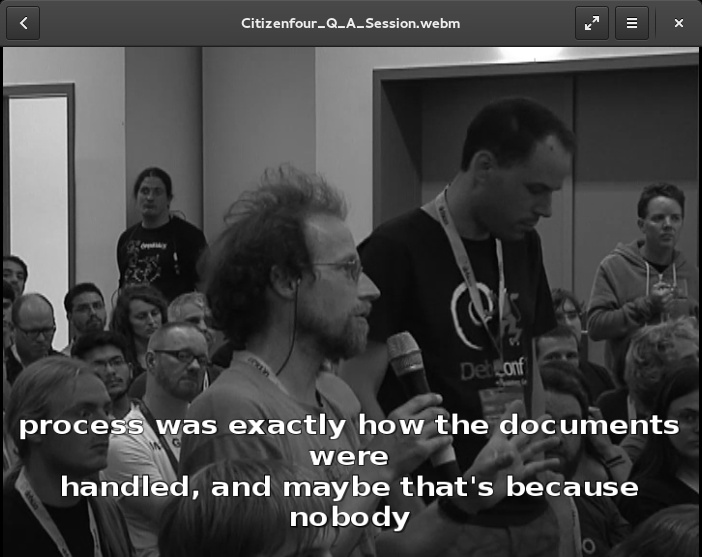
\includegraphics[width=0.5\hsize]{image201510/subtitle_mono.png}
\end{center}
\caption{$B;zKkIU$-:F@8Nc(B}
\end{figure}

\subsection{$B:#2s$N%S%G%*>R2p(B}

 $B:#2s>R2pM=Dj$N6qBNE*$J%;%C%7%g%sL>$O!"(B

\begin{itemize}
\item Stretching out for trustworthy reproducible builds
\item Thanks for maintaining a desktop environment. But is it accessible?
\end{itemize}

$B$H$J$j$^$9!#(B

\subsection{Stretching out for trustworthy reproducible builds}

 $B%I%$%D$NM-L>$J(BChaos Computer Club\footnote{Wikipedia-jp$B$G0z$$$F$_$F2<$5$$!#%I%$%D$NM-L>$J%3%s%T%e!<%?5;=Q$N%(%-%9%Q!<%H=8CD!#(B}$B$K$b=jB0$5$l$F$$$k(BDebian$B3+H/<T$i$K$h$k!"(BReproducible Builds$B$K$D$$$F$N%;%C%7%g%s$G$9!#(B

\begin{figure}[H]
\begin{center}
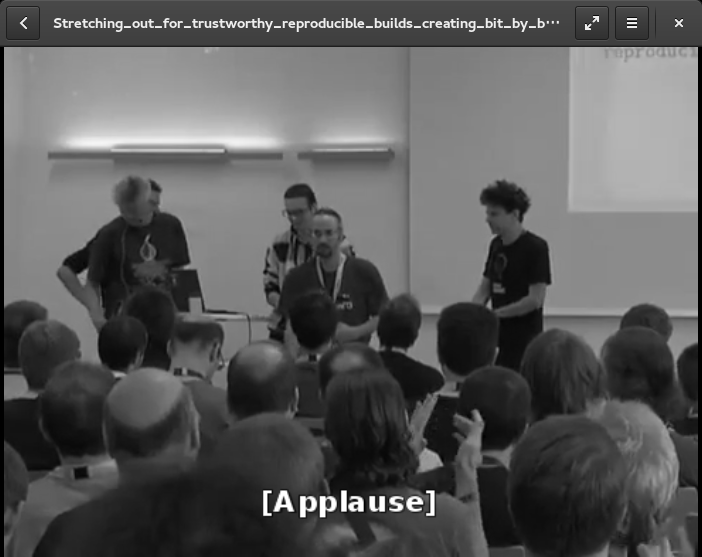
\includegraphics[width=0.5\hsize]{image201510/reproduct_mono.png}
\end{center}
\caption{Stretching out for trustworthy($BN,(B)$B$NH/I=(B}
\end{figure}

$BG!2?$K%S%G%*$NFbMF$r$+$$$D$^$s$G>R2p$7$^$9!#(B

\subsubsection{$BF05!(B}

 \begin{itemize}
 \item The 31st Chaos Communication Congress (31C3)\footnote{Chaos Computer Club$B<g:E$NKhG/9T$o$l$k%$%Y%s%H(B}$B$K$F!"%Q%C%1!<%8$N%P%$%J%j$K%H%m%$$NLZGO$,9*L/$K;E3]$1$i$l$F$$$k$+!)$rD4$Y$k$K$O(BReproducible Builds$B$r$7$?$[$&$,NI$$$H$$$&H/I=$r9T$C$?$H$N$3$H$G$9!#(B
\item 31C3$B$N$o$:$+?t%+7n8e$K:#EY$O(BEdward Snowden$B$5$s$K$h$j!"(BCIA$B$N(BStrawhourse$B$H$$$&%3!<%IL>$K4X$9$k(BCIA conference 2012$B$NFbItJ8>O$,%j!<%/$5$l$^$7$?!#FbMF$O!"(BMacOS/iOS$B$N(BSDK$B$KITEv$J2~B$$r9T$$!"@8@.$5$l$k%P%$%J%j$K(BCIA$B$,MxMQ$9$k$?$a$N%H%m%$$NLZGO$r;E3]$1$k$H$$$&6C$/$Y$-FbMF$G$7$?!#$3$l$K$h$j!"(BReproducible Builds$B$,1W!95^L3$K$J$C$?$H$N$3$H$G$9!#$J$*!"%j!<%/J8>O$O!"(B\url{https://theintercept.com/document/2015/03/10/strawhorse-attacking-macos-ios-software-development-kit/}$B$G;2>H$G$-$^$9!#(B
 \end{itemize}

\subsubsection{$B%;%-%e%j%F%#0J30$NNI$$E@(B}

\begin{itemize}
 \item $B%S%k%I4D6-$K$h$i$:F1$8%P%$%J%j$,$G$-$k!"$^$?!"%/%m%9%S%k%I$N3NG'$,$G$-$k$h$&$K$J$k!"(B
 \item Debug package$B$,$$$D$G$b!J%P%$%J%j:n$C$?$"$H$G$b!K:n$l$k$H$+!"(B
 \item FTBFS\footnote{Fails To Build From Source$B$NN,(B}$B$,Aa$/$o$+$k$H$+!"(B
 \item $B%P!<%8%g%s>e$2$?;~$N(B.deb$B$N:9J,$,>.$5$/$J$k$H$N$3$H$G$9!#(B
 \end{itemize}

\subsubsection{$B8=:_$N(BReproducible Builds$B>u67$O<!$NDL$j(B}

 \begin{itemize}
 \item Bitcoin/Tor/Coreboot$B$O40N;$7$F$$$k!#(B
 \item Debian/FreeBSD/NetBSD/OpenWrt$B$O?J9TCf!#(B
 \end{itemize}

\subsubsection{$B9)IW$H6lO+(B}
 
\begin{itemize}
\item $B4D6-JQ?t(BSOURCE\_DATE\_EPOCH$B$K;~9o(B($B%(%]%C%/IC(B)$B$r;XDj$9$k$H!"$=$N;~9o$G%S%k%I$7$?$h$&$K%S%k%I$9$k$h$&$KMM!9$J%D!<%k$r2~B$$7(Bupstream$B$XDs6!$7<h$j9~$s$G$b$i$C$?$=$&$G$9!#$J$*!"$3$l$@$1$G$OB-$i$J$$%Q%C%1!<%8$,Bt;3$"$C$?$i$7$/!"%S%k%I$NF|IU$,Kd$a9~$^$l$kItJ,$r(BReproducible Builds$B=PMh$J$$$H(BBTS$B$7$?$j$7$FBP:v$bB??t$7$?$H$N$3$H$G$9!#(B
\item tar$B$K%S%k%I4D6-$NETEY$N%f!<%6L>!"%0%k!<%WL>$,:.$8$C$F$7$^$&7o$rBP:v$7$?$=$&$G$9!#(B
\item $B%U%!%$%k%7%9%F%`$H(Blocale$B4D6-JQ?t(B(LANG,LC\_ALL$BJQ?t(B)$B$H$N0c$$$K$h$k%=!<%H$N?6$kIq$$$N0c$$!"%W%m%0%i%`$N=PNO$,0[$J$C$F$7$^$&7o$NBP:v$r$7$?$=$&$G$9!#(B
\end{itemize}

$B8@$o$l$F$_$k$H!V$J$k$[$I!*!W$H5$$,$D$/;v$P$+$j$G!"9M$($F$_$l$PAjEv$K6lO+$9$k$h$&$JFbMF$P$+$j$G$7$?!#(B

\subsubsection{$B;kD08e$N=j46(B}

$B$h$/!"9+$G$O4JC1$K(BReproducible Builds$B$O!"%Q%C%1!<%8$N%;%-%e%j%F%#3NG'$N0Y$H4JC1$K>R2p$5$l$^$9$,!"<B$O(BDebian$B$r9=@.$9$k=EMW$J%=%U%H%&%'%"!&%Q%C%1!<%8$NB?$/$K<j$r2C$($J$1$l$P<B8=$G$-$J$$$H$$$&BgJQ$J0N6H$r2L$?$7$F$$$?$H$$$&FbMF$G$7$?!#;W$o$:!"$3$l$i$N0N6H$KGo<j$r$7$?$/$J$j$^$7$?!#(B

\subsection{Thanks for maintaining a desktop environment. But is it accessible?}

 Debian Project$B$K$F(BAccessibility$B$rC4Ev$5$l$F$$$kJ}$NH/I=$H$J$j$^$9!#(B
Accessibility$B$K4X$7$F$N8=>u$H6lO+$,$o$+$kH/I=FbMF$H$J$C$F$$$^$9!#(B

 $B%W%l%<%s;qNA$O!'(B\url{http://brl.thefreecat.org/2015-08-22-debconf.pdf}

\begin{figure}[H]
\begin{center}
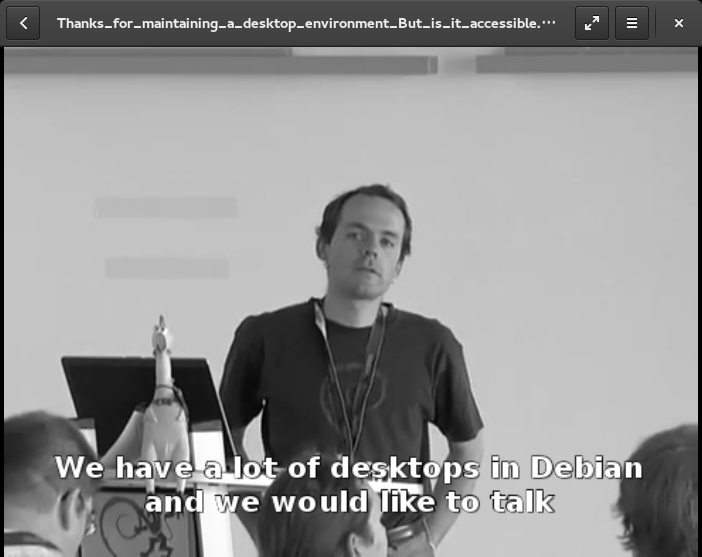
\includegraphics[width=0.5\hsize]{image201510/accessibility_mono.png}
\end{center}
\caption{Thanks for maintaining a desktop...($BN,(B)$B$NH/I=(B}
\end{figure}

\subsubsection{Accessibility$B$K$D$$$F$&$C$+$j$9$k$HK:$l$,$A$K$J$kBgJQ=EMW$J;v(B}

$B!!(BFree Software$B$O!"LdBj$,$"$C$?$j!"5$$KF~$i$J$+$C$?$i!"<+J,$GD>$;$k$H$$$&$3$H$,4pK\$G$"$k$,!"(BAccessibility$B$N5!G=$rI,MW$H$7$F$$$k?M$O!"4pK\<#$7$?$/$F$bD>$;$J$$>l9g$,B?$$$N$G!"%3%_%e%K%F%#!<$K$h$k=$@5!&2~A1$,I,?\$G$9!#(B

\subsubsection{Linux Desktop$B4D6-$N(BAccessibility$B$N8=>u(B}

\begin{itemize}
  \item Linux$B$GF0:n$9$k(BDesktop$B4D6-$O!"(BGNOME$B$,(BAccessibility$B$,:G$b$h$/$G$-$F$$$k>u67$G$9!#(B
  \item $B$7$+$7$J$,$i!"(BGNOME3$B$r;}$C$F$7$F$b!"(BWindows$B$KHf$Y$k$H(B10$BG/C10L$GCY$l$F$*$j!"(BApple$B$N@=IJ$KHf$Y$k$H@P4o;~Be$NBeJ*$H8@$o$l$F$b;EJ}$,L5$$>u67$G$9!#(B
  \item $B<e;k$N?M$K$O!"9g@.2;@<$K$h$k%5%]!<%H$O87$7$$>l9g!J$=$b$=$bH/2;$7$K$/$$%o!<%I$N>l9g$J$I!K$,$"$k$?$a!"M}A[E*$K$O!"(BPiezo braille cell$B$r%5%]!<%H$9$Y$-$G$9!#(B
\end{itemize}

\subsubsection{Linux Desktop$B4D6-$N(BAccessibility$B$N8=>u$N;EAH$_$H3+H/J}K!(B}

$B@h$N%W%l%<%s;qNA!"5Z$S!"%S%G%*$K$F(B

\begin{itemize}
  \item Linux$B$N(BAccessibility$B$N%U%l!<%`%o!<%/!"(B
  \item Linux$B$N(BAccessibility$B$N%F%9%H4D6-$J$I(B
 \end{itemize}

$B$,>R2p$5$l$F$$$^$9!#@h=R$N%W%l%<%s;qNA$r;2>H$/$@$5$$!#(BAccessibility$B$,$I$N$h$&$K$G$-$F$$$F!"$I$&%F%9%H$9$Y$-$+$K$D$$$F!"Hs>o$KNI$$;qNA$H$J$C$F$$$^$9!#(B

\subsection{$B$*$o$j$K(B}

$B!!;fLL$N4X78$G:#2s$O%;%C%7%g%s$r#2$D$N$_>R2p$7$^$7$?$,!"B>$K$bHs>o$K6=L#?<$$%;%C%7%g%s$,$"$j$^$9!#$J$K$V$s1Q8l$N%;%C%7%g%s$J$N$G!"8+$FM}2r$9$k$N$K6lO+$9$k>u67$G$9$,!"$=$NEXNO$rJ'$C$?$@$1$N<}3O$,$"$k$N$,!"(BDebconf$B$N%S%G%*$G$9!#@'Hs!"#1$D8+$F!"FbMF$r9M$($F$_$^$;$s$+!)$-$C$H!":#$^$G8+$($F$$$?@$3&$,$,$i$C$HJQ$o$k$h$&$JBN83$,=PMh$k$H;W$C$F$$$^$9!#(B

%2015KOF
\dancersection{Debian $B$H(B arm64$B%5%]!<%H(B}{$B4d>>(B $B?.MN(B}

  \subsection{arm64}
  \begin{itemize}
  \item Debian 8.0 $B$+$i(B arm64 $B%5%]!<%H$,F~$C$?(B
  \item Debian $B$G%5%]!<%H$9$k(B ARM $B%"!<%-%F%/%A%c(B
$B!!(B\begin{itemize}
  \item armel\\
  32bit / litte endian / ARMv5t

  $B8E$$(BNAS(QNAP$B!"(BBuffalo$B!"(Betc)$B$d%k!<%?$G;HMQ$5$l$F$$$k(B ARM SoC$B$GMxMQ2DG=!#(B

  \item armhf\\
  32bit / litte endian / ARMv7 + VFP3$B!JIbF0>.?tE@1i;;%f%K%C%H!K(B

  Raspberry Pi \textcolor{red}{2} $B$J$I$GMxMQ2DG=!#(B

  \item arm64 $\leftarrow$ \textcolor{red}{New!}

  \end{itemize}

  \item Raspbian

  \begin{itemize}
  \item 32bit / litte endian / ARMv6 + VFP2$B!JIbF0>.?tE@1i;;%f%K%C%H!K(B

       Raspberry Pi \textcolor{red}{1} $B$J$I$GMxMQ2DG=!#(B
  \item Raspbian in not Debian

  \end{itemize}

  \end{itemize}





  \subsection{arm64}
  \begin{itemize}
  \item ARMv8 (ARM Version 8)
  \end{itemize}
  \begin{center}
  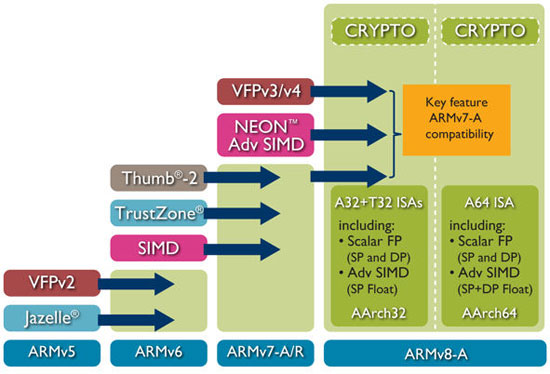
\includegraphics[width=0.7\hsize]{image201511/V5_to_V8_Architecture.jpg}
  \end{center}



  \subsection{arm64}

\begin{minipage}{0.7\hsize}
\begin{itemize}
\item ARMv8 (ARM Version 8)
\item $B%*%j%8%J%k%3%"$H$7$F$O(BCortex-A57$B!"(BARM Cortex-A53$B$H(BCortex-A72$B$,$"$k(B
\item $B@5<0L>>N$O(BAArch64
\item Linux kernel $B$G$O(B $B$o$+$j$K$/$$$H$$$&$3$H$G(B arm64 $B$K(B\\
\url{https://lkml.org/lkml/2012/7/15/133}
\item Debian $B$b$3$l$KDI=>$7$F(B arm64 $B$H$7$?(B
\item $B%3%s%Q%$%i$J$I$N%H%j%W%l%C%H$O(B aarch64-linux-gnu 
\item GCC $B$NDj5A$O(B \_\_aarch64\_\_ 
\end{itemize}
\end{minipage}
\begin{minipage}{0.25\hsize}

\includegraphics[width=0.8\hsize]{image201511/1254383-arm-aarch-64-300x250.jpg}
\end{minipage}




  \subsection{arm64}

  \begin{center}
  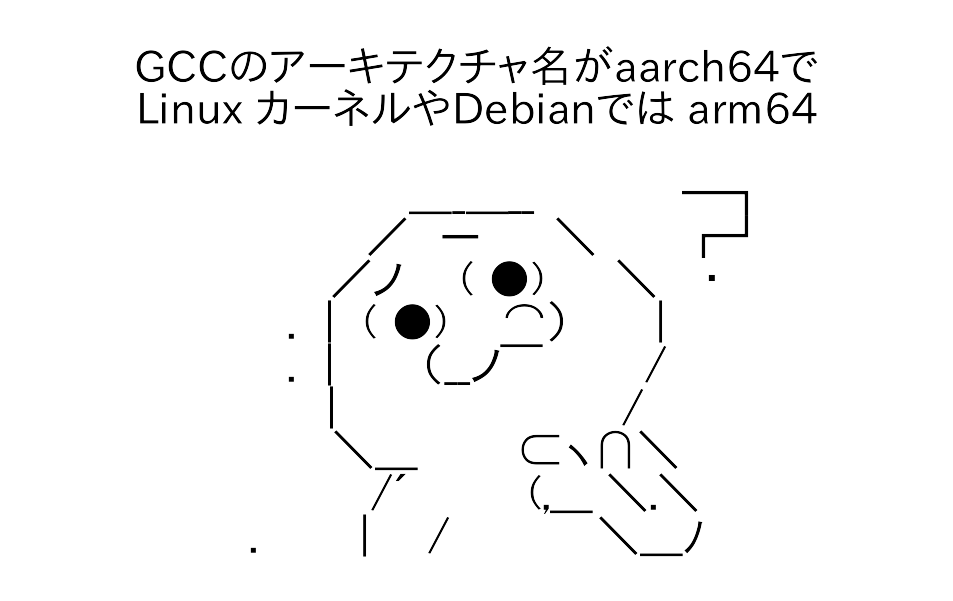
\includegraphics[width=0.8\hsize]{image201511/yaruoAA.png}
  \end{center}



  \subsection{Debian ARM $B3+H/BN@)(B}

  \begin{itemize}
  \item 2012 $BG/$+$i3+H/3+;O(B
  \item $B3+H/$K;22C$7$F$$$kB?$/$N(BDebian Developer $B$,(B Linaro $B=jB0(B

   Steve McIntyre$B!"(B Wookey$B!"(BRiku Voipio $B$J$I(B

  \item GCC/binutils:

    Matthias Klose (GCC Upstream, Ubuntu Developer $B$G$b$"$k(B)
  \item libc:
    
    Aurelien Jarno$B!"(Blibc $B%a%s%F%J%A!<%`(B
  \item Linux kernel:

    Ben Hutchings(Linux 3.2 LTS $B%a%s%F%J(B)$B!"(BIan Campbell$B!J(BXen$B!"(BAllwinner SoCs $B4X(B
$BO"!K!"$=$NB>Bg@*(B

  % \item Linaro $B$N@.2L$,(B Debian $B$H(B Ubuntu$B$K2s$k%5%$%/%k$,$G$-$F$$$k(B

  \end{itemize}



  \subsection{Debian ARM $B3+H/BN@)(B}

  \begin{itemize}
  \item Buildd: Applied Micro $B$N(B X-gene $B$r;H$C$?%5!<%P$G1?MQCf(B
     \url{https://buildd.debian.org/status/architecture.php?a=arm64&suite=sid}
  \item SoC: X-C1 / 2.4Ghz / 8$B%3%"(B $BFH<+%3%"(B

  \begin{center}
  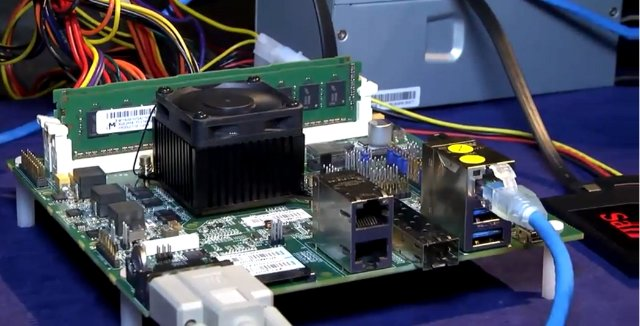
\includegraphics[width=0.7\hsize]{image201511/x-gene.jpg}
  \end{center}

  \end{itemize}



%FIXME not find image201511/graph-week-big.png
%
%  \subsection{Debian ARM $B3+H/BN@)(B}
%
%  \begin{center}
%  \includegraphics[width=0.7\hsize]{image201511/graph-week-big.png}
%  \end{center}
%
%



  \subsection{$B%/%m%9%3%s%Q%$%k4D6-(B}
  \begin{itemize}
  \item Jessie $B%j%j!<%98e(BDebian$B$N%/%m%9%3%s%Q%$%k4D6-$,JQ$o$C$?(B
  \item $B:#$^$G$O(BEmdebian$B$+$iDs6!$5$l$F$$$k%Q%C%1!<%8$r;H$&$+!"%f!<%6<+?H$G%Q%C%1(B
$B!<%82=$9$kI,MW$,$"$C$?!#(B$\leftarrow$ $B$a$s$I$$!#(B

  \item GCC$B%a%s%F%J$K$h$j%/%m%9%3%s%Q%$%kMQ%Q%C%1!<%8$,Ds6!$5$l$k$h$&$K(B

  \begin{itemize}
    \item $B%/%m%9MQ(Bbinutils $\rightarrow$ binutils $B%=!<%9%Q%C%1!<%8(B
    \item $B%/%m%9MQ(Blibc $\rightarrow$ cross-toolchain-base $B%=!<%9%Q%C%1!<%8(B
    \item $B%/%m%9MQ(BGCC $\rightarrow$ gcc-5-cross $B%=!<%9%Q%C%1!<%8(B

\begin{commandline}
    $ sudo apt-get install gcc-5-aarch64-linux-gnu
\end{commandline}

  \end{itemize}

  \item $B%j%j!<%9BP>]30$N%"!<%-%F%/%A%c$OL$%5%]!<%H(B
  \end{itemize}



  \subsection{$B%f!<%6%i%s%I%$%a!<%8(B}
  \begin{itemize}
  \item $B%$%s%9%H!<%i$,MQ0U$5$l$F$$$k(B \\
	  \url{https://www.debian.org/CD/http-ftp/#stable}
  \item cdebootstrap $B$r;H$&$N$,4JC1(B

\begin{commandline}
   $ sudo cdebootstrap --foreign --arch arm64 \
         jessie /tmp/root http://http.debian.net/debian/
\end{commandline}
  \end{itemize}




  \subsection{$B%5%]!<%H%\!<%I(B}
  \begin{itemize}
  \item Debian $B$G$O(B ARM $B%j%U%!%l%s%9%\!<%I!J(BJuno$B!K$H(B X-gene$B!J(BApplied Micro$B!K$N$_%5%]!<%H!#(B
  \item arm64 $B$N%\!<%I$OCMCJ$,%/%=9b$$!J(B10$BK|1_0J>e!K>e$KF~<j@-$,0-$$!#(B
%FIXME not find image201511/juno.jpg 
%  \begin{center}
%    \includegraphics[width=0.5\hsize]{image201511/juno.jpg}
%  \end{center}
  
  \end{itemize}



  \subsection{$B%5%]!<%H%\!<%I(B}
  \begin{itemize}
    \item 96boards (Linaro Community Board Program) $B$+$iF~<j$9$k$N$,$h$5$2!#Ls(B1$BK|1_!#(B
    \begin{center}
    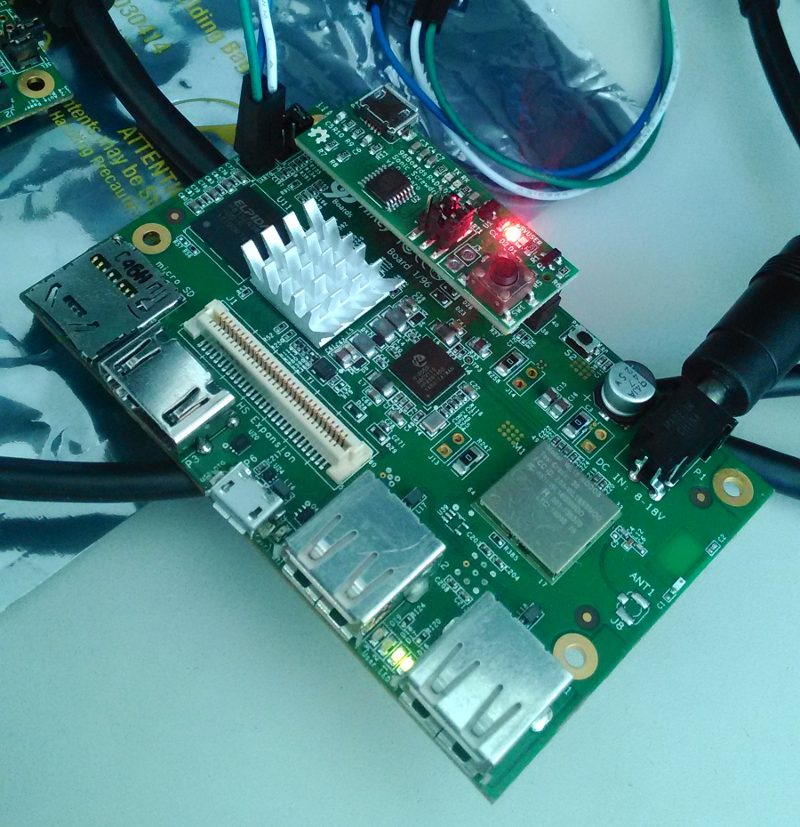
\includegraphics[width=0.3\hsize]{image201511/hikey.png}
    \end{center}
    \begin{itemize}
    \item Linux $B%+!<%M%k%Q%C%1!<%8$,99?7$5$l<!Bh!"(BDebian $B$G$b%5%]!<%H$9$kM=Dj!#(B
    \end{itemize}
  \item QEMU $B$r;H$C$F3+H/$9$k$3$H$b2DG=!#$?$@$7(B QEMU 2.0$B0J9_!#(B
  \end{itemize}



  \subsection{$B%Y%s%A%^!<%/(B}

\begin{table}[htb]
  \begin{tabular}{|l|l|l||l|} \hline
    $B%Y%s%A%^!<%/(B  & Raspberry Pi 2 & ODROID-XU4 & Hikey  \\ \hline \hline
    Dhrystone-2 & 1006.6 & 3994.1 & \textcolor{red}{2943.7} \\ \hline
    Double-Precision Whetstone & 361.0 & 1024.9 & \textcolor{red}{680.3} \\ \hline
    Nbench 2.2.3 Integer  & 20.419 & 61.227  & \textcolor{red}{30.803} \\ \hline
    Nbench 2.2.3 FP  & 8.434 & 25.369 & \textcolor{red}{11.889} \\ \hline
  \end{tabular}
\end{table}

\begin{itemize}
\item Raspberry Pi 2: Broadcom BCM2836 900MHz  ARM Cortex-A7 4 core
\item ODROID-XU4: Samsung Exynos5422 Cortex-A15 2Ghz and Cortex-A7 Octa core CPUs
\item Hikey: HiSilicon Kirin 6220 Cortex-A53 1.2Ghz Octa core
\end{itemize}

 \begin{center}
 \textcolor{red}{\texttt{ODROID-XU4 > Hikey > Raspberry Pi 2}}
 \end{center}



%
%  \subsection{$B%Y%s%A%^!<%/(B}
%  \begin{center}
%  \includegraphics[width=0.3\hsize]{image201511/20110809aa_20110809185955.jpg}
%  \end{center}
%


  \subsection{$B%Y%s%A%^!<%/(B}
  \begin{itemize}
  \item $B$V$C$A$c$1(B $B$$$^$N$H$3$m(B ARMv7 $B$NJ}$,B.$$!#(B
  \item Cortex $B$,CY$$$H$$$&OC$b!#FH<+%3%"$N(BSoC$B$O$=$3$=$3B.$$!#(B
  \item $B$H$$$C$F$b$3$N$^$^(B32bit ARM $B$r;H$C$F$b(B2038$BG/LdBj$,$,$,!*(B
  \item Cortex-A72 $B$K4|BT!#(B
  \end{itemize}



  \subsection{$B$^$H$a(B}
  \begin{itemize}
  \item Debian $B$G$O(B ARM64 $B$,4{$K;H$($k4D6-$,@0$C$F$$$k!#(B
  \item Upstream $B$d(B $B<~JUAH?%$H$NO"7H$b==J,!#(B
  \item $B%/%m%9%3%s%Q%$%k4D6-$b%*%U%#%7%c%k$G%5%]!<%H$5$l$k$h$&$K$J$j!":#$^$G0J>e$K3+H/$7$d$9$/$J$C$F$$$k!#(B
  \item $B%\!<%I$N6!5kLdBj$,%M%C%/!#0lHL8~$1$O(B 96boards $BMj$j!#(B
  \item $B>e5-$NM}M3$b$"$j!"%5%]!<%H%\!<%I$O>/$J$$!#:#8e4hD%$C$FA}$d$7$^$9!#(B
  \end{itemize}


%201509tokyo
\dancersection{Debian $B%Q%C%1!<%8%s%0F;>l(B git buildpackage$B$N;H$$J}(B}{$B4d>>(B $B?.MN(B}

Debian $B%Q%C%1!<%8%s%0%A%e!<%H%j%"%k(B\footnote{https://www.debian.org/doc/manuals/packaging-tutorial/packaging-tutorial.ja.pdf}$B$G$"$^$j2r@b$5$l$F$$$J$$(B gbp (git
buildpackage) $B$N4pK\E*$J;H$$J}$K$D$$$F@bL@$9$k!#(B

\subsection{VCS $B$G4IM}$7$J$$>l9g(B}

\begin{center}
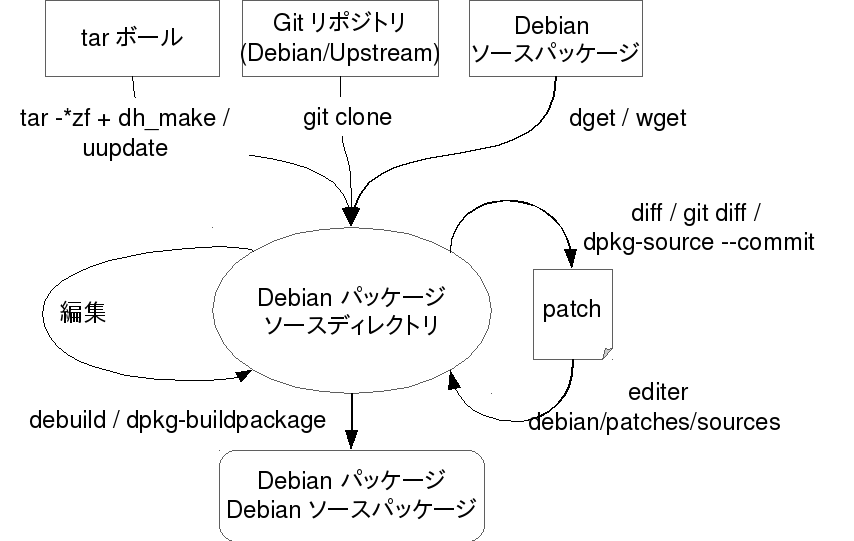
\includegraphics[width=0.8\hsize]{image201509/gbp-images0_mono.png}
\end{center}


\subsection{VCS $B$G4IM}$9$k>l9g(B}
\begin{center}
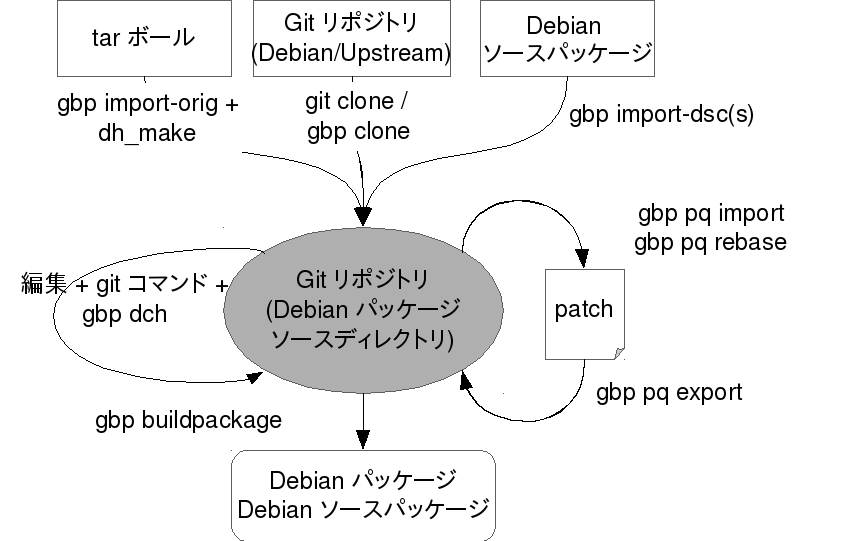
\includegraphics[width=0.8\hsize]{image201509/gbp-images1_mono.png}
\end{center}

\subsection{Upstream $B$+$i(B tar $B%\!<%k$,%j%j!<%9$5$l$F$$$k>l9g(B}

Upstream $B$+$i(Btar$B%\!<%k$,%j%j!<%9$5$l$F$$$k>l9g!"(B
tar $B%\!<%k$r(BGit$B%j%]%8%H%j$K%3%_%C%H$7$?8e!"%Q%C%1!<%82=$r9T$&!#(B


\begin{itemize}
\item tar $B%\!<%k$r%@%&%s%m!<%I$9$k(B

\begin{commandline}
$ wget package-name-0.0.1.tar.gz
\end{commandline}

\item Git$B%j%]%8%H%j$r:n@.$9$k(B

\begin{commandline}
$ git init package-name
$ cd package-name
\end{commandline}

$BI,MW$G$"$l$P(B git config $B$G(B Git $B$N@_Dj$rJQ99$9$k!#(B
\end{itemize}

\begin{itemize}
\item tar $B%\!<%k$r;XDj$7$F!"%=!<%9%3!<%I$r(B Git $B$K%3%_%C%H$9$k(B

\begin{commandline}
$ gbp import-orig --pristine-tar \
	../package-name-0.0.1.tar.gz
$ git tag 
$ upstream/0.0.1
$ git branch
* master
  upstream
\end{commandline}
\end{itemize}

\begin{itemize}
\item Upstream$B$N%3!<%I$r$O(B upstream $B%V%i%s%A$G4IM}$5$l!"F1;~$K%?%0$,@_(B
$BDj$5$l$k!#(B
\item pristine-tar $B%*%W%7%g%s$O%*%j%8%J%k$N(Btar$B%\!<%k$N:9J,$rJ]B8$9$k$?$a$N;EAH$_$rM-8z(B
$B$K$9$k!#(BUpstream$B$N%3!<%I$O(B upstream $B%V%i%s%A$G4IM}$5$l!"(BDebian $B%Q%C%1!<%8$r(B
$B:n@.$9$k$H$-$K!"$=$3$+$i(B orig.tar.gz $B%U%!%$%k$r:n@.$9$k!#$3$N;~$K:n@.$5$l$k%U%!%$%k(B
$B$,F1$8$b$N$K$J$i$J$$>l9g$,$"$k!#(BDebian $B$G$O(B
$B<h$j9~$s$@(B tat.gz $B%U%!%$%k$N%O%C%7%eCM$H(BDebian $B%=!<%9%Q%C%1!<%8$H$7$F%"%C%W%m!<%I$5$l$k(B
tar.gz $B%U%!%$%k$,F1$8$G$"$kI,MW$,$"$k$?$a!"K\%*%W%7%g%s$rMQ$$$F(B orig.tar.gz$B$H$N:9J,$r(B
$B%P%$%J%j%Q%C%A$H$7$FJ]B8$7!"(Borig.tar.gz$B$r9=C[$9$kEY$K:FE,MQ$9$k$3$H$G!"%O%C%7%eCM(B
$B$,F1$8(Borig.tar.gz$B$r:F9=C[$G$-$k$h$&$K$7$F$$$k!#(B
\end{itemize}

\begin{itemize}
\item dh\_make $B$G(B debian $B%G%#%l%/%H%j$N?w7A$r:n@.$9$k(B 

\begin{commandline}
$ dh_make -p package-name_0.0.1
\end{commandline}

\item debian $B%G%#%l%/%H%jFb$r$$$m$$$mJQ99$9$k(B

\begin{commandline}
$ $B$$$m$$$m=$@5(B
$ git add debian
$ git commit
\end{commandline}
\end{itemize}

\begin{itemize}
\item $B%Q%C%1!<%82=:n6H$,$G$-$?$i(B $B%Q%C%1!<%8$r9=C[$9$k(B

\begin{commandline}
$ gbp buildpackage --git-pristine-tar
\end{commandline}

\item piuparts $B$J$I$G%$%s%9%H!<%k!"%"%s%$%s%9%H!<%k$N%F%9%H(B

\item $B:G8e$K%/%j!<%s$J4D6-$G%S%k%I%F%9%H(B

\begin{commandline}
$ git-pbuilder
or
$ gbp buildpackage --git-pbuiler --git-pristine-tar
\end{commandline}
\end{itemize}

\begin{itemize}
\item $B%?%0$r@_Dj$7$F(B $B%j%b!<%H%j%]%8%H%j$K%W%C%7%e$9$k(B

\begin{commandline}
$ gbp buildpackage --git-tag-only
$ git push
\end{commandline}

\end{itemize}

\subsection{upstream $B$K99?7$,$"$C$?>l9g(B}


\begin{itemize}
\item upstream $B$N(Btar $B%\!<%k$r<hF@$9$k(B

\begin{commandline}
$ wget package-name-0.0.2.tar.gz
\end{commandline}

\item tar $B%\!<%k$r;XDj$7$F%j%]%8%H%j$K%=!<%9%3!<%I$r%3%_%C%H$9$k(B

\begin{commandline}
$ gbp import-orig --pristine-tar \
		../package-name-0.0.2.tar.gz
\end{commandline}

\texttt{--uscan} $B%*%W%7%g%s$G%@%&%s%m!<%I(B $\rightarrow$ $B%3%_%C%H$,0lEY$K$G$-$k!#(B
$B$^$?!"%=!<%9%3!<%I$O<+F0E*$K%^!<%8$5$l$^$9!#%^!<%8$7$?$/$J$$>l9g$O(B
\texttt{--no-merge} $B$r;XDj$7$F<B9T$9$k!#(B
\end{itemize}

\begin{itemize}
\item debian/changelog $B$r=$@5(B

\begin{commandline}
$ dch -i
or
$ gbp dch 
\end{commandline}

\item $B%Q%C%1!<%8$r%S%k%I(B

\begin{commandline}
$ gbp buildpackage --git-pristine-tar \
		--git-pristine-tar-commit
\end{commandline}

\end{itemize}


% -------------------------------------------------

\subsection{Upstream $B$,(B Git $B$G4IM}$5$l$F$$$k>l9g(B}

\begin{itemize}
\item  Upstream $B$G$O(B tar $B%\!<%k$G%j%j!<%9$5$l$:!"(BGit$B$N%?%0$N$_$G%j%j!<%9$5$l$k>l9g(B
$B$b$"$k!#(B
\item Github $B$G3+H/$5$l$F$$$k%W%m%8%'%/%H$,NI$$Nc!#(B
\item $B$3$N$h$&$J>l9g$O(B $B%j%]%8%H%j$r%/%m!<%s$7$?8e!"(BDebian$BFH<+$N%V%i%s%A%k!<%k$rMQ$$$F(B
$B%=!<%9%Q%C%1!<%8$N4IM}$r9T$&!#(B
\end{itemize}


\begin{itemize}

\item $B%j%]%8%H%j$r%/%m!<%s$7!":n@.$5$l$?%G%#%l%/%H%j$K0\F0$9$k(B

\begin{commandline}
$ git clone git://example.org/git/package-name.git
$ cd package-name
\end{commandline}
\end{itemize}

\begin{itemize}
\item $B%Y!<%9$K$7$?$$%P!<%8%g%s$N%3!<%I$r%A%'%C%/%"%&%H$9$k(B

\begin{commandline}
$ git reset --hard 0.0.1
\end{commandline}
\end{itemize}

\begin{itemize}
\item $B%?%0$r@_Dj$9$k(B

\begin{commandline}
$ git tag upstream/0.0.1
\end{commandline}

upstream $B%M!<%`%9%Z!<%9$O(B gbp $B%G%U%)%k%H;2>H@h!#(BUpstream$B$N%?%0$r;H$$$?$$>l9g(B
$B$dFH<+$N%M!<%`%9%Z!<%9$r;H$$$?$$>l9g$O(B gbp $B$N(B upstream-tag $B$,MxMQ$G$-$^$9!#(B

\begin{commandline}
[git-buildpackage]
upstream-tag = v%(version)s
\end{commandline}
\end{itemize}

\begin{itemize}
\item dh\_make $B$G(B debian $B%G%#%l%/%H%j$N?w7A$r:n@.$9$k(B

\begin{commandline}
$ dh_make -p package-name_0.0.1
\end{commandline}
\end{itemize}

\begin{itemize}
\item debian $B%G%#%l%/%H%jFb$r$$$m$$$mJQ99$9$k(B

\begin{commandline}
$ $B$$$m$$$m=$@5(B
$ git add debian
$ git commit
\end{commandline}
\end{itemize}

\begin{itemize}
\item $B%Q%C%1!<%82=:n6H$,$G$-$?$i(B $B%Q%C%1!<%8$r9=C[$9$k(B

\begin{commandline}
$ gbp buildpackage --git-pristine-tar \
		--git-pristine-tar-commit
\end{commandline}

tar $B%\!<%k$r;H$&>l9g$H0[$J$k$N$O(B\texttt{--git-pristine-tar-commit} $B%*%W%7%g%s(B
$B$r;XDj$9$k$3$H!#$3$N%*%W%7%g%s$r;XDj$9$k$3$H$K$h$C$F%?%0$+$i(B orig.tar.gz $B$r@8@.(B
$B$9$k!#(B
\end{itemize}

\begin{itemize}
\item piuparts $B$J$I$G%$%s%9%H!<%k!"%"%s%$%s%9%H!<%k$N%F%9%H(B

\item $B:G8e$K%/%j!<%s$J4D6-$G%S%k%I%F%9%H(B

\begin{commandline}
$ git-pbuilder
or
$ gbp buildpackage --git-pbuilder
\end{commandline}
\end{itemize}

\begin{itemize}
\item $B%?%0$r@_Dj$7$F(B $B%j%b!<%H%j%]%8%H%j$K%W%C%7%e$9$k(B

\begin{commandline}
$ gbp buildpackage --git-tag-only
$ git push
\end{commandline}

\end{itemize}

\subsection{upstream $B$K99?7$,$"$C$?>l9g(B}


\begin{itemize}
\item upstream $B$N%j%]%8%H%j>pJs$r<hF@$9$k(B

\begin{commandline}
$ git remote update
\end{commandline}
\end{itemize}

\begin{itemize}
\item $BJQ99$r%^!<%8(B

\begin{commandline}
$ git tag upstream/0.0.2 0.0.2
$ git merge upstream/0.0.2
\end{commandline}
\end{itemize}

\begin{itemize}
\item debian/changelog $B$r=$@5(B

\begin{commandline}
$ dch -i
or
$ gbp dch
\end{commandline}
\end{itemize}

\begin{itemize}
\item $B%Q%C%1!<%8$r%S%k%I(B

\begin{commandline}
$ gbp buildpackage --git-pristine-tar\
		--git-pristine-tar-commit
\end{commandline}

\end{itemize}

\subsection{$B%"%C%W%9%H%j!<%`$N%=!<%9%3!<%IJQ99(B}

\begin{enumerate}
\item gbp pq import
\item Upstream $B%=!<%9%3!<%I$N=$@5(B
\item git commit
\item gbp pq export
\item git commit
\end{enumerate}

\begin{center}
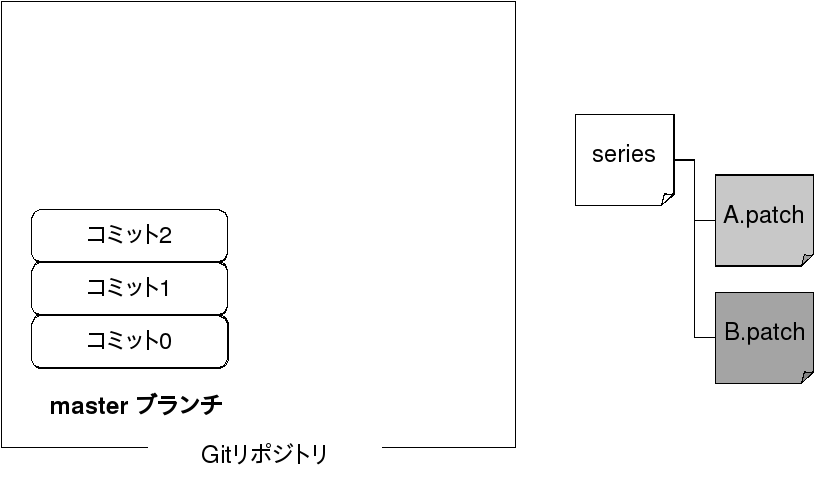
\includegraphics[width=0.8\hsize]{image201509/gbp-pq0_mono.png}
\end{center}


\subsection{gbp pq import}

  \begin{enumerate}
   \item HEAD $B$r(Bpatch-queue/master $B%V%i%s%A$H$7$F%A%'%C%/%"%&%H(B
   \item debian/patches/series $B$K$"$k%Q%C%A$r%3%_%C%H(B
  \end{enumerate}

\begin{center}
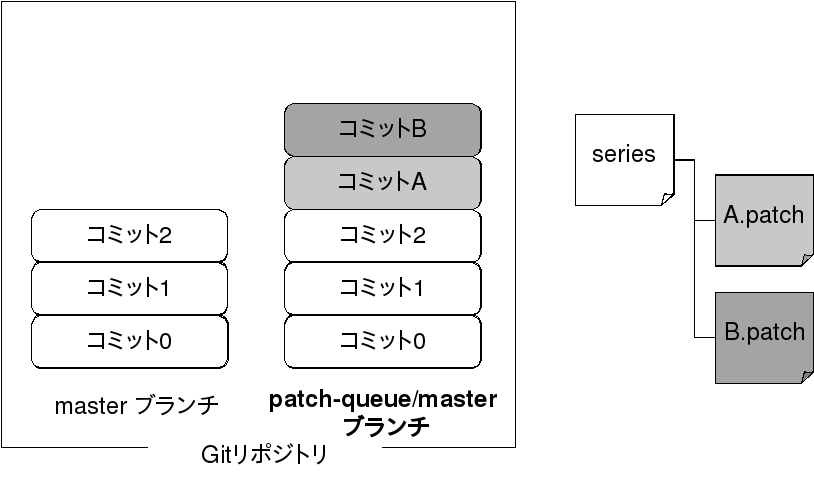
\includegraphics[width=0.8\hsize]{image201509/gbp-pq1_mono.png}
\end{center}


\subsection{$B=$@5(B \& git commit}

  \begin{enumerate}
   \item Upstream $B%=!<%9%3!<%I$N=$@5(B
   \item git commit
  \end{enumerate}

\begin{center}
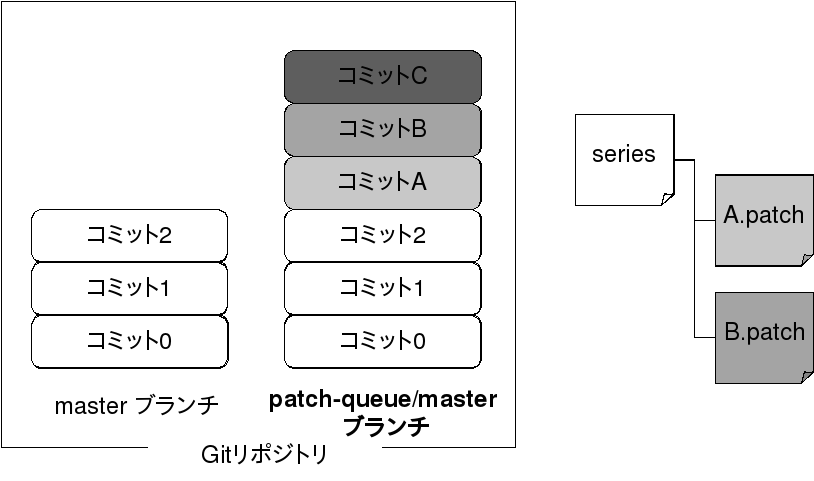
\includegraphics[width=0.8\hsize]{image201509/gbp-pq2_mono.png}
\end{center}


\subsection{gbp pq export}
  \begin{enumerate}
   \item patch-queue/master $B$H(B master $B%V%i%s%A$N:9J,$r%Q%C%A$H$7$F(B debian/patches $B$K=PNO(B
   \item debian/patches/series $B$r99?7(B
   \item master $B%V%i%s%A$r%A%'%C%/%"%&%H(B
  \end{enumerate}

\begin{center}
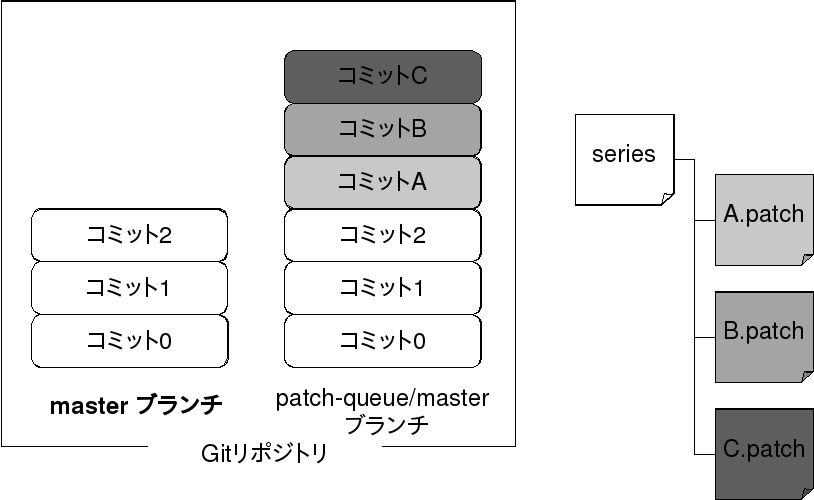
\includegraphics[width=0.8\hsize]{image201509/gbp-pq3_mono.png}
\end{center}
  
  

\subsection{git commit}
  \begin{enumerate}
   \item $B%Q%C%A99?7$r%j%]%8%H%j$K%3%_%C%H(B
  \end{enumerate}

\begin{center}
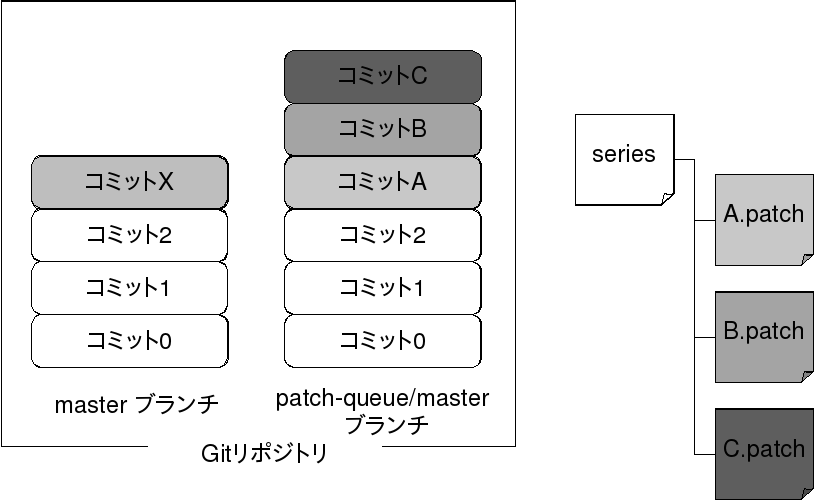
\includegraphics[width=0.8\hsize]{image201509/gbp-pq4_mono.png}
\end{center}

\subsection{$B$^$H$a(B}

\begin{itemize}
\item gbp (git buildpackage)$B$O%G%U%!%/%H%9%?%s%@!<%H(B
\item gbp import-* $B$G%j%]%8%H%j<h$j9~$_(B
  
  \texttt{--pristine-tar} $B$rK:$l$:$K(B
\item gbp dch $B$G(B debian/changelog $B$r99?7(B
\item gbp buildpackage $B$G%Q%C%1!<%8%S%k%I(B
\item gbp pq $B$G%Q%C%AA`:n(B
\end{itemize}

%-------------------------------------------------------------------------------
\dancersection{Debian Trivia Quiz}{}
%-------------------------------------------------------------------------------

$B$H$3$m$G!"$_$J$5$s(B Debian $B4XO"$NOCBj$K$*$$$D$$$F$$$^$9$+!)(BDebian$B4XO"$NOC(B
$BBj$O%a!<%j%s%0%j%9%H$r$h$s$G$$$k$HDI@W$G$-$^$9!#$?$@$h$s$G$$$k$@$1$G$O$O(B
$B$j$"$$$,$J$$$N$G!"M}2rEY$N%F%9%H$r$7$^$9!#FC$K0l?M$@$1$G$O0UL#$,$o$+$i$J(B
$B$$$H$3$m$b$"$k$+$bCN$l$^$;$s!#$_$s$J$G0l=o$KFI$s$G$_$^$7$g$&!#(B

$B:#2s$N=PBjHO0O$O(B\url{debian-devel-announce@lists.debian.org} $B$d(B \url{debian-devel@lists.debian.org}$B$KEj9F$5$l$?(B
$BFbMF$H(BDebian Project News$B$+$i$G$9!#(B

\begin{multicols}{2}
\input{image201506/quiz.tex}
\input{image201507/quiz.tex}
\input{image201511/quiz.tex}
\end{multicols}

%for less page
%\printindex

% $BLdBj$H2sEz$,F1$8$_$R$i$-$K$J$i$J$$$h$&$K$9$k(B
\cleartooddpage
%-------------------------------------------------------------------------------
\dancersection{Debian Trivia Quiz $BLdBj2sEz(B}{}
%-------------------------------------------------------------------------------

 Debian Trivia Quiz $B$NLdBj2sEz$G$9!#(B
 $B$"$J$?$O2?Ld$o$+$j$^$7$?$+!)(B \\
 %$B2sEz$O(Bdebianmeetingresume2014-fuyu.jqz$B$H$$$&%U%!%$%k$K@8@.$5$l$k$N$G!"(B
 %$B$=$l$r<jF0$G%3%T%Z$7$F;H$&!#(B
 % $B$3$3$+$i%3%T%Z(B
 % FIXME $BLdBj$,A4It$O$$$C$?$i%3%T%Z$9$k$3$H(B
 %(progn (next-line 1)(insert-file "debianmeetingresume2013-fuyu.jqz") )
1. A $B$$$/$D$+$N@H<e@-BP:v$d!"%P%0%U%#%C%/%9$,9T$o$l$?%Q%C%1!<%8$,<h$j9~$^$l$^$7$?!#(BDebian 8(Jessie)$B$r%$%s%9%H!<%k$7$?$P$+$j$N?M$O!"AaB.%"%C%W%0%l!<%I$7$^$7$g$&!*(B\\
2. B $B?k$K(B22,000$B$rD6$($?$=$&$G$9!#%P%$%J%j%Q%C%1!<%8$N?t$O(B45,542$B$H$N;v!#1W!9A}$($F$$$/$h$&$G$9!#(B\\
3. C $B:#$^$G!"%G%P%C%0%7%s%\%k$O(B-dbg$B%Q%C%1!<%8$GG[I[$5$l$F$$$^$7$?!#$7$+$7$J$,$i!"$3$A$i$N(B-dbg$B%Q%C%1!<%8$OB>$N%G%P%C%0$H$O2?$i4X78$N$J$$%Q%C%1!<%8$H0l=o$K(Bmirror$B$5$l$k$?$a!"(B-dbg$B%Q%C%1!<%8$NMxMQ<T$,$H$F$b>/$J$$$K$b$+$+$o$i$:!"(Bmirror$B@h$N;q8;$r$=$NJ,>CHq$7$F$7$^$$$^$9!#:#2s$NDs0F$O!"%G%P%C%0%7%s%\%k(B.ddeb$B$H$$$&%Q%C%1!<%8$K$7$F$7$^$$!"$3$A$i$N%Q%C%1!<%8$K$D$$$F$O(Bmirror$B@h$b8:$i$9!J$7$J$$!)!K$H$$$&;v$r8!F$$9$k$b$N$G$9!#(B\\
4. B jessie$B$GMxMQ$G$-$J$$%Q%C%1!<%8$r!"(Bwheezy-backports$B$+$i$4$C$=$j>C$7$?$H$N$3$H$G$9!#(Bbackports$B$K4^$^$l$k$I$N%Q%C%1!<%8$,$I$&$J$C$F$$$k$+!)$I$&$7$FM_$7$$$+!)$K$D$$$F$O!"(Bfreeze$B$N4|4V$H(Bfreeze$B8e$N$o$:$+$J4|4V$N4V$K!"(Bbackport$BC4Ev$+$i(Bbackports$B%A!<%`$K<+H/E*$K%?%$%`%j!<$KAjCL$7$FMh$FM_$7$$$H$N4+9p$b9T$o$l$^$7$?!#(B\\
5. C $B$^$:$O!"(BDebian sid$B$G$O!"(Bgcc 5/libstdc++6$B$G%3%s%Q%$%k!&F0:n=PMh$k$h$&$K%Q%C%1!<%8%a%s%F%J$NJ}$O=$@5BP1~$r$7$FM_$7$$;]$N%"%J%&%s%9$,$"$j$^$7$?!#:#2s!"(BABI$B%Y!<%9$G$bJQ99$K$J$C$?$j!"(BC++11$B$KBP1~$H$J$C$?$j$G1F6A$,=t!9H/@8$7$^$9!#$^$?!"$3$N1F6A$G!"(BGFortran$BB&$b(Bmodule 14$B$X0\9T$H$J$k$N$G!"(BGFortran$B$r;H$C$F$$$k%Q%C%1!<%8%a%s%F%J$bBP1~$,I,MW$H$N$3$H$G$9!#(B\\
6. A libav*$B$H$$$&%^%k%A%a%G%#%"$N%G!<%?$r07$&%i%$%V%i%j$J$N$G$9$,!"0lC6(Blibav.org$B$,Ds6!$7$F$$$k$b$N$KJQ99$H$J$C$?$N$G$9$,!"$^$?(BFFmpeg$B$,Ds6!$7$F$$$k$b$N$KLa$C$F$-$?>u67$G$9!#5DO@$N%5%^%j$O(B https://wiki.debian.org/Debate/libav-provider/ffmpeg\\
7. B $B%9%l$N=;?M$N<ALd$K!"(BDPL$B$,(BArchLinux$B$,@($$$HEz$($F$$$^$7$?!#(Bwiki$B$N=<<B$V$j$,$H$K$+$/AG@2$i$7$$$H$N$3$H!#(B\\
8. C Debian$B%"!<%+%$%V$r(Bgit$B$GA`:n$G$-$k%D!<%k$N(Bdgit$B$,(B1.0$B$,%j%j!<%9$5$l$?$H$N$3$H$G$9!#AaB.(Bdebian sid$B$K<}O?$5$l$F$$$^$9!#(Bdgit clone package$BL>$H$9$k$H!"(Bhttps://git.dgit.debian.org/ $B$G4IM}$5$l$F$$$k$b$N$,<j85$K(Bclone$B$5$l$^$9!#(B\\
9. C Strech$B$GMxMQ$5$l$k$G$"$m$&!"%$%s%9%H!<%i%W%m%0%i%`$N&A(B1$B$,%j%j!<%9$5$l$^$7$?!#$b$A$m$s!"(BStrech$B$,%j%j!<%9$5$l$?$o$1$G$O$J$$$N$GCm0U!#JQ99E@$O?t!9$"$j!"%G%U%)%k%H$N(BCPU$B%"!<%-%F%/%A%c$,(Bamd64$B$K$J$C$?$j$7$?!#>\$7$/$O(Bdebian-devel-announce$B$r;2>H(B\\
10. C 2015/10/22$B$N(BDPN$B$N%a!<%k$+$i!"=>MhN.$l$F$$$?(BDPN$B$N%a!<%k$N9=@.$,:~?7$5$l$^$7$?!#$3$A$i$KH<$$!"%;%-%e%j%F%#$K$D$$$F$N%"%J%&%s%9$H!"?7$7$$(BDD/DM$B$N%"%J%&%s%9$O!"(BDPN$B$N%a!<%k$K$O4^$^$l$:!"(BWeb$B%Z!<%8$K7G:\$5$l$k$N$_$H$J$j$^$7$?!#(B\\
11. A XMPP$B$O%*!<%W%s$J%$%s%9%?%s%H%a%C%;%s%8%c!<MQ%W%m%H%3%k$N#1$D!#$J$*!"(BDebian$B4X78<T$NMxMQ$K$"$?$C$F>\$7$/$O!"(Bhttp://rtc.debian.org$B$r;2>H!#(B\\
12. B 2$BL>$[$I!"(BDebian Developer$B$NJ}$G(Btechnical comittee$B$G3hLv$G$-$kJ}Jg=8$H$N$3$H$G$9!#8=?&(Btechnical comittee$B$N?M$i$,!"(B2015/12/31$B$GG$4|$,@Z$l$F$7$^$&$H$$$&$3$H$G!"$=$l$^$G$K8uJd<T$r5s$2$kI,MW$,$"$k$H$N$3$H$G$9!#(B

% add page to even number

\newpage
\thispagestyle{empty}\mbox{}%$BN"I=;f$NN"B&$N%Z!<%8!"?';f(B

\begin{center}
$BK\;qNA$N%i%$%;%s%9$K$D$$$F(B
\end{center}

$BK\;qNA$O%U%j!<!&%=%U%H%&%'%"$G$9!#$"$J$?$O!"(BFree Software
Foundation $B$,8xI=$7$?(BGNU GENERAL PUBLIC LICENSE$B$N!V%P!<%8%g%s#2!W$b$7$/$O$=$l0J9_(B
$B$,Dj$a$k>r9`$K=>$C$FK\%W%m%0%i%`$r:FHRI[$^$?$OJQ99$9$k$3$H$,$G$-(B
$B$^$9!#(B

$BK\%W%m%0%i%`$OM-MQ$H$O;W$$$^$9$,!"HRI[$K$"$?$C$F$O!";T>l@-5Z$SFC(B
$BDjL\E*E,9g@-$K$D$$$F$N0EL[$NJ]>Z$r4^$a$F!"$$$+$J$kJ]>Z$b9T$J$$$^(B
$B$;$s!#>\:Y$K$D$$$F$O(BGNU GENERAL PUBLIC LICENSE $B$r$*FI$_$/$@$5$$!#(B

\begin{multicols}{2}
 \begin{fontsize}{6}{6}
 \begin{verbatim}
		    GNU GENERAL PUBLIC LICENSE
		       Version 2, June 1991

 Copyright (C) 1989, 1991 Free Software Foundation, Inc.
	51 Franklin St, Fifth Floor, Boston, MA  02110-1301  USA
 Everyone is permitted to copy and distribute verbatim copies
 of this license document, but changing it is not allowed.

			    Preamble

  The licenses for most software are designed to take away your
freedom to share and change it.  By contrast, the GNU General Public
License is intended to guarantee your freedom to share and change free
software--to make sure the software is free for all its users.  This
General Public License applies to most of the Free Software
Foundation's software and to any other program whose authors commit to
using it.  (Some other Free Software Foundation software is covered by
the GNU Library General Public License instead.)  You can apply it to
your programs, too.

  When we speak of free software, we are referring to freedom, not
price.  Our General Public Licenses are designed to make sure that you
have the freedom to distribute copies of free software (and charge for
this service if you wish), that you receive source code or can get it
if you want it, that you can change the software or use pieces of it
in new free programs; and that you know you can do these things.

  To protect your rights, we need to make restrictions that forbid
anyone to deny you these rights or to ask you to surrender the rights.
These restrictions translate to certain responsibilities for you if you
distribute copies of the software, or if you modify it.

  For example, if you distribute copies of such a program, whether
gratis or for a fee, you must give the recipients all the rights that
you have.  You must make sure that they, too, receive or can get the
source code.  And you must show them these terms so they know their
rights.

  We protect your rights with two steps: (1) copyright the software, and
(2) offer you this license which gives you legal permission to copy,
distribute and/or modify the software.

  Also, for each author's protection and ours, we want to make certain
that everyone understands that there is no warranty for this free
software.  If the software is modified by someone else and passed on, we
want its recipients to know that what they have is not the original, so
that any problems introduced by others will not reflect on the original
authors' reputations.

  Finally, any free program is threatened constantly by software
patents.  We wish to avoid the danger that redistributors of a free
program will individually obtain patent licenses, in effect making the
program proprietary.  To prevent this, we have made it clear that any
patent must be licensed for everyone's free use or not licensed at all.

  The precise terms and conditions for copying, distribution and
modification follow.

		    GNU GENERAL PUBLIC LICENSE
   TERMS AND CONDITIONS FOR COPYING, DISTRIBUTION AND MODIFICATION

  0. This License applies to any program or other work which contains
a notice placed by the copyright holder saying it may be distributed
under the terms of this General Public License.  The "Program", below,
refers to any such program or work, and a "work based on the Program"
means either the Program or any derivative work under copyright law:
that is to say, a work containing the Program or a portion of it,
either verbatim or with modifications and/or translated into another
language.  (Hereinafter, translation is included without limitation in
the term "modification".)  Each licensee is addressed as "you".

Activities other than copying, distribution and modification are not
covered by this License; they are outside its scope.  The act of
running the Program is not restricted, and the output from the Program
is covered only if its contents constitute a work based on the
Program (independent of having been made by running the Program).
Whether that is true depends on what the Program does.

  1. You may copy and distribute verbatim copies of the Program's
source code as you receive it, in any medium, provided that you
conspicuously and appropriately publish on each copy an appropriate
copyright notice and disclaimer of warranty; keep intact all the
notices that refer to this License and to the absence of any warranty;
and give any other recipients of the Program a copy of this License
along with the Program.

You may charge a fee for the physical act of transferring a copy, and
you may at your option offer warranty protection in exchange for a fee.

  2. You may modify your copy or copies of the Program or any portion
of it, thus forming a work based on the Program, and copy and
distribute such modifications or work under the terms of Section 1
above, provided that you also meet all of these conditions:

    a) You must cause the modified files to carry prominent notices
    stating that you changed the files and the date of any change.

    b) You must cause any work that you distribute or publish, that in
    whole or in part contains or is derived from the Program or any
    part thereof, to be licensed as a whole at no charge to all third
    parties under the terms of this License.

    c) If the modified program normally reads commands interactively
    when run, you must cause it, when started running for such
    interactive use in the most ordinary way, to print or display an
    announcement including an appropriate copyright notice and a
    notice that there is no warranty (or else, saying that you provide
    a warranty) and that users may redistribute the program under
    these conditions, and telling the user how to view a copy of this
    License.  (Exception: if the Program itself is interactive but
    does not normally print such an announcement, your work based on
    the Program is not required to print an announcement.)

These requirements apply to the modified work as a whole.  If
identifiable sections of that work are not derived from the Program,
and can be reasonably considered independent and separate works in
themselves, then this License, and its terms, do not apply to those
sections when you distribute them as separate works.  But when you
distribute the same sections as part of a whole which is a work based
on the Program, the distribution of the whole must be on the terms of
this License, whose permissions for other licensees extend to the
entire whole, and thus to each and every part regardless of who wrote it.

Thus, it is not the intent of this section to claim rights or contest
your rights to work written entirely by you; rather, the intent is to
exercise the right to control the distribution of derivative or
collective works based on the Program.

In addition, mere aggregation of another work not based on the Program
with the Program (or with a work based on the Program) on a volume of
a storage or distribution medium does not bring the other work under
the scope of this License.

  3. You may copy and distribute the Program (or a work based on it,
under Section 2) in object code or executable form under the terms of
Sections 1 and 2 above provided that you also do one of the following:

    a) Accompany it with the complete corresponding machine-readable
    source code, which must be distributed under the terms of Sections
    1 and 2 above on a medium customarily used for software interchange; or,

    b) Accompany it with a written offer, valid for at least three
    years, to give any third party, for a charge no more than your
    cost of physically performing source distribution, a complete
    machine-readable copy of the corresponding source code, to be
    distributed under the terms of Sections 1 and 2 above on a medium
    customarily used for software interchange; or,

    c) Accompany it with the information you received as to the offer
    to distribute corresponding source code.  (This alternative is
    allowed only for noncommercial distribution and only if you
    received the program in object code or executable form with such
    an offer, in accord with Subsection b above.)

The source code for a work means the preferred form of the work for
making modifications to it.  For an executable work, complete source
code means all the source code for all modules it contains, plus any
associated interface definition files, plus the scripts used to
control compilation and installation of the executable.  However, as a
special exception, the source code distributed need not include
anything that is normally distributed (in either source or binary
form) with the major components (compiler, kernel, and so on) of the
operating system on which the executable runs, unless that component
itself accompanies the executable.

If distribution of executable or object code is made by offering
access to copy from a designated place, then offering equivalent
access to copy the source code from the same place counts as
distribution of the source code, even though third parties are not
compelled to copy the source along with the object code.

  4. You may not copy, modify, sublicense, or distribute the Program
except as expressly provided under this License.  Any attempt
otherwise to copy, modify, sublicense or distribute the Program is
void, and will automatically terminate your rights under this License.
However, parties who have received copies, or rights, from you under
this License will not have their licenses terminated so long as such
parties remain in full compliance.

  5. You are not required to accept this License, since you have not
signed it.  However, nothing else grants you permission to modify or
distribute the Program or its derivative works.  These actions are
prohibited by law if you do not accept this License.  Therefore, by
modifying or distributing the Program (or any work based on the
Program), you indicate your acceptance of this License to do so, and
all its terms and conditions for copying, distributing or modifying
the Program or works based on it.

  6. Each time you redistribute the Program (or any work based on the
Program), the recipient automatically receives a license from the
original licensor to copy, distribute or modify the Program subject to
these terms and conditions.  You may not impose any further
restrictions on the recipients' exercise of the rights granted herein.
You are not responsible for enforcing compliance by third parties to
this License.

  7. If, as a consequence of a court judgment or allegation of patent
infringement or for any other reason (not limited to patent issues),
conditions are imposed on you (whether by court order, agreement or
otherwise) that contradict the conditions of this License, they do not
excuse you from the conditions of this License.  If you cannot
distribute so as to satisfy simultaneously your obligations under this
License and any other pertinent obligations, then as a consequence you
may not distribute the Program at all.  For example, if a patent
license would not permit royalty-free redistribution of the Program by
all those who receive copies directly or indirectly through you, then
the only way you could satisfy both it and this License would be to
refrain entirely from distribution of the Program.

If any portion of this section is held invalid or unenforceable under
any particular circumstance, the balance of the section is intended to
apply and the section as a whole is intended to apply in other
circumstances.

It is not the purpose of this section to induce you to infringe any
patents or other property right claims or to contest validity of any
such claims; this section has the sole purpose of protecting the
integrity of the free software distribution system, which is
implemented by public license practices.  Many people have made
generous contributions to the wide range of software distributed
through that system in reliance on consistent application of that
system; it is up to the author/donor to decide if he or she is willing
to distribute software through any other system and a licensee cannot
impose that choice.

This section is intended to make thoroughly clear what is believed to
be a consequence of the rest of this License.

  8. If the distribution and/or use of the Program is restricted in
certain countries either by patents or by copyrighted interfaces, the
original copyright holder who places the Program under this License
may add an explicit geographical distribution limitation excluding
those countries, so that distribution is permitted only in or among
countries not thus excluded.  In such case, this License incorporates
the limitation as if written in the body of this License.

  9. The Free Software Foundation may publish revised and/or new versions
of the General Public License from time to time.  Such new versions will
be similar in spirit to the present version, but may differ in detail to
address new problems or concerns.

Each version is given a distinguishing version number.  If the Program
specifies a version number of this License which applies to it and "any
later version", you have the option of following the terms and conditions
either of that version or of any later version published by the Free
Software Foundation.  If the Program does not specify a version number of
this License, you may choose any version ever published by the Free Software
Foundation.

  10. If you wish to incorporate parts of the Program into other free
programs whose distribution conditions are different, write to the author
to ask for permission.  For software which is copyrighted by the Free
Software Foundation, write to the Free Software Foundation; we sometimes
make exceptions for this.  Our decision will be guided by the two goals
of preserving the free status of all derivatives of our free software and
of promoting the sharing and reuse of software generally.

			    NO WARRANTY

  11. BECAUSE THE PROGRAM IS LICENSED FREE OF CHARGE, THERE IS NO WARRANTY
FOR THE PROGRAM, TO THE EXTENT PERMITTED BY APPLICABLE LAW.  EXCEPT WHEN
OTHERWISE STATED IN WRITING THE COPYRIGHT HOLDERS AND/OR OTHER PARTIES
PROVIDE THE PROGRAM "AS IS" WITHOUT WARRANTY OF ANY KIND, EITHER EXPRESSED
OR IMPLIED, INCLUDING, BUT NOT LIMITED TO, THE IMPLIED WARRANTIES OF
MERCHANTABILITY AND FITNESS FOR A PARTICULAR PURPOSE.  THE ENTIRE RISK AS
TO THE QUALITY AND PERFORMANCE OF THE PROGRAM IS WITH YOU.  SHOULD THE
PROGRAM PROVE DEFECTIVE, YOU ASSUME THE COST OF ALL NECESSARY SERVICING,
REPAIR OR CORRECTION.

  12. IN NO EVENT UNLESS REQUIRED BY APPLICABLE LAW OR AGREED TO IN WRITING
WILL ANY COPYRIGHT HOLDER, OR ANY OTHER PARTY WHO MAY MODIFY AND/OR
REDISTRIBUTE THE PROGRAM AS PERMITTED ABOVE, BE LIABLE TO YOU FOR DAMAGES,
INCLUDING ANY GENERAL, SPECIAL, INCIDENTAL OR CONSEQUENTIAL DAMAGES ARISING
OUT OF THE USE OR INABILITY TO USE THE PROGRAM (INCLUDING BUT NOT LIMITED
TO LOSS OF DATA OR DATA BEING RENDERED INACCURATE OR LOSSES SUSTAINED BY
YOU OR THIRD PARTIES OR A FAILURE OF THE PROGRAM TO OPERATE WITH ANY OTHER
PROGRAMS), EVEN IF SUCH HOLDER OR OTHER PARTY HAS BEEN ADVISED OF THE
POSSIBILITY OF SUCH DAMAGES.

		     END OF TERMS AND CONDITIONS

	    How to Apply These Terms to Your New Programs

  If you develop a new program, and you want it to be of the greatest
possible use to the public, the best way to achieve this is to make it
free software which everyone can redistribute and change under these terms.

  To do so, attach the following notices to the program.  It is safest
to attach them to the start of each source file to most effectively
convey the exclusion of warranty; and each file should have at least
the "copyright" line and a pointer to where the full notice is found.

    <one line to give the program's name and a brief idea of what it does.>
    Copyright (C) <year>  <name of author>

    This program is free software; you can redistribute it and/or modify
    it under the terms of the GNU General Public License as published by
    the Free Software Foundation; either version 2 of the License, or
    (at your option) any later version.

    This program is distributed in the hope that it will be useful,
    but WITHOUT ANY WARRANTY; without even the implied warranty of
    MERCHANTABILITY or FITNESS FOR A PARTICULAR PURPOSE.  See the
    GNU General Public License for more details.

    You should have received a copy of the GNU General Public License
    along with this program; if not, write to the Free Software
    Foundation, Inc., 51 Franklin St, Fifth Floor, Boston, MA  02110-1301 USA


Also add information on how to contact you by electronic and paper mail.

If the program is interactive, make it output a short notice like this
when it starts in an interactive mode:

    Gnomovision version 69, Copyright (C) year  name of author
    Gnomovision comes with ABSOLUTELY NO WARRANTY; for details type `show w'.
    This is free software, and you are welcome to redistribute it
    under certain conditions; type `show c' for details.

The hypothetical commands `show w' and `show c' should show the appropriate
parts of the General Public License.  Of course, the commands you use may
be called something other than `show w' and `show c'; they could even be
mouse-clicks or menu items--whatever suits your program.

You should also get your employer (if you work as a programmer) or your
school, if any, to sign a "copyright disclaimer" for the program, if
necessary.  Here is a sample; alter the names:

  Yoyodyne, Inc., hereby disclaims all copyright interest in the program
  `Gnomovision' (which makes passes at compilers) written by James Hacker.

  <signature of Ty Coon>, 1 April 1989
  Ty Coon, President of Vice

This General Public License does not permit incorporating your program into
proprietary programs.  If your program is a subroutine library, you may
consider it more useful to permit linking proprietary applications with the
library.  If this is what you want to do, use the GNU Library General
Public License instead of this License.
 \end{verbatim}
 \end{fontsize}
\end{multicols}

\begin{center}
$B%=!<%9%3!<%I$K$D$$$F(B
\end{center}

$B%=!<%9%3!<%I$O(B Git $B$r;H$C$F(B\url{git://anonscm.debian.org/tokyodebian/monthly-report.git}
$B$+$i%@%&%s%m!<%I$G$-$^$9!#0J2<$KJ}K!$r<($7$^$9!#(B

\begin{commandline}
$ git clone git://anonscm.debian.org/tokyodebian/monthly-report.git
\end{commandline}
%$

%\newpage
\cleartoevenpage

\newpage
%\thispagestyle{empty}\mbox{}
%\newpage

\thispagestyle{empty}
{
\large
\begin{itembox}{\bf $B!X$"$s$I$-$e$a$s$F$C$I(B $B$G$S$"$s!Y$K$D$$$F(B}
$BK\=q$O!"El5~$*$h$S4X@><~JU$GKh7n9T$J$o$l$F$$$k!XEl5~%(%j%"(B Debian $BJY6/2q!Y$*$h$S(B
$B!X4X@>(B Debian $BJY6/2q!Y$G(B
$B;HMQ$5$l$?;qNA!&>.%M%?!&I,;&5;$J$I$r0l:}$K$^$H$a$?$b$N$G$9!#(B
% FIXME: $BHO0O$r=$@5$9$k$3$H!#(B
$B<}O?HO0O$O(B2015/06$B!A(B2015/11$B$^$G(B
$BEl5~%(%j%"$OBh(B127$B2s$+$iBh(B133$B2s$^$G$*$h$S!"(B
$B4X@>%(%j%"$OBh(B99$B2s$+$iBh(B104$B2s$^$G(B($B4X@>Bh(B99-101$B2s(B,104$B2s$O$b$/$b$/2q!"(BLT$B$N$?$a<}O?L5$7(B)$B!#(B
$BFbMF$OL5J]>Z!"$D$C$3$_$J$I$,$"$l$PJY6/2q$K$F!#(B
\end{itembox}
}

\vspace*{13cm}
{\color{dancerlightblue}\rule{\hsize}{1mm}}
\vspace{2mm}

\includegraphics[width=2cm]{image200502/openlogo-nd.eps}
\noindent \Large \bf $B$"$s$I$-$e$a$s$F$C$I(B $B$G$S$"$s(B 2015$BG/E_9f(B\\
\noindent \normalfont 2015$BG/(B12$B7n(B31$BF|(B \hspace{5mm}  $B=iHGBh(B1$B:~H/9T(B\\
\noindent \normalfont $BEl5~%(%j%"(B Debian $BJY6/2q(B/$B4X@>(BDebian $BJY6/2q(B $B!JJT=8!&0u:~!&H/9T!K(B\\
{\color{dancerdarkblue}\rule{\hsize}{1mm}}

\end{document}
